\chapter{Controlling the ROV} \label{cha:controller} \index{Open-Loop Control} \index{Controller} \index{Feedback Linearisation} \index{Feedback Control}
Automatic control is a way of regulating a process without direct human interaction. The complexity can vary from decentralised proportional, integral and derivative controllers (\abbrPID{}s) to more advanced model-based control methods, such as model predictive control (\abbrMPC) \citep{reglerteori}. 

There are two main concepts of control, open-loop and feedback control \citep{reglerteknik}. An open-loop controller is a controller that computes its output based on a model of the system. A disadvantage of open-loop controllers is that they require exact knowledge of the controlled system \citep{reglerteknik}. \Figureref{fig:control_system_open} illustrates the open-loop control scheme used in the \abbrROV. 

\begin{figure}
	\centering
		\begin{tikzpicture}[auto, thick, node distance=2cm,>=latex',
			 block/.style  = {draw, rectangle,minimum height=3em, minimum width=6em},
			 sum/.style    = {draw, circle, inner sep=0pt, text width=4mm,align=center, node distance=1cm},
			 input/.style  = {coordinate},
			 output/.style = {coordinate},
			 pinstyle/.style = {pin edge={to-,thin,black}}]
			 
		    \node [input, name=input] {};
		    \node [block, right of=input, node distance=3cm] (controller) {F};
		    \node [block, right of=controller, node distance=3cm] (system) {\abbrROV};
		
		    \draw [->] (controller) -- node[name=u] {$u$} (system);
		    \node [output, right of=system] (output) {};
		
		    \draw [draw,->] (input) -- node {$x_{\text{ref}}$} (controller);
		    \draw [->] (system) -- node [name=y] {$y$}(output);
		\end{tikzpicture}
	\caption{The open-loop control scheme used in the \abbrROV. The control block F can be any type of open-loop control. Notice that this is an ideal case where no disturbances affect the system.}
	\label{fig:control_system_open}
\end{figure}

A feedback controller uses measurements of the outputs in a system to get a desired behaviour. One such method is error-controlled regulation, where the difference between the desired value, the setpoint, of an output and its measured or estimated value is used for control \citep{reglerteknik}. The feedback control scheme used in the \abbrROV can be seen in \Figureref{fig:control_system}. 

Similarly to an open-loop controller, a feedback controller can use a model of the system. Using a model of the controlled system in the control structure can produce better performance and compensate for unwanted effects such as non-linearities. Compensating for non-linearities is desired due to the fact that a lot of control principles are based on linear systems \citep{reglerteori}. 

\begin{figure}
	\centering
		\begin{tikzpicture}[auto, thick, node distance=2cm,>=latex',
			 block/.style  = {draw, rectangle,minimum height=3em, minimum width=6em},
			 sum/.style    = {draw, circle, inner sep=0pt, text width=4mm,align=center, node distance=1cm},
			 input/.style  = {coordinate},
			 output/.style = {coordinate},
			 pinstyle/.style = {pin edge={to-,thin,black}}]
			 
		    \node [input, name=input] {};
		    \node [sum, right of=input] (sum) {+};
		    \node [block, right of=sum] (controller) {F};
		    \node [block, right of=controller, node distance=3cm] (system) {\abbrROV};
		
		    \draw [->] (controller) -- node[name=u] {$u$} (system);
		    \node [output, right of=system] (output) {};
		    \node [block, below of=u] (sensorfusion) {Observer};
		
		    \draw [draw,->] (input) -- node {$x_{\text{ref}}$} (sum);
		    \draw [->] (sum) -- node {$e$} (controller);
		    \draw [->] (system) -- node [name=y] {$y$}(output);
		    \draw [->] (y) |- (sensorfusion);
		    \draw [->] (sensorfusion) -| node[pos=0.99] {$-$} 
		        node [near end] {$\hat{x}$} (sum);
		\end{tikzpicture}
	\caption{The feedback control scheme used in the \abbrROV. The controller F can be any of the controllers discussed in this chapter. The observer in the \abbrROV is the sensor fusion described in \Chapterref{cha:sensor_fusion}. Notice that this is an ideal case where no disturbances effect the system.}
	\label{fig:control_system}
\end{figure}


%%%%%%%%%%%%%%%%%%%%%%%%%%%%%%%%%%%%%%%
\section{Open-Loop Control} \label{sec:openloop} \index{Open-Loop Control} \index{thrust allocation} \index{thruster geometry}
The open-loop control of the \abbrROV consists of a static thrust-allocation matrix which is
\begin{equation} \label{eq:pinv}
    \thrusterGeometryOnes[+] = \thrusterGeometryOnes[T](\thrusterGeometryOnes \thrusterGeometryOnes[T])^{-1}
\end{equation}
where $\thrusterGeometryOnes$ describes how the actuators effect the \abbrROV \citep{thrustallocation}. If the thrust-geometry matrix is chosen as
\begin{equation} \label{eq:Tones}
    \thrusterGeometryOnes = 
    \begin{bmatrix}
    0  & 0  & 1 & 1  &  0 &  0 \\
    0  & 0  & 0 & 0  &  0 & -1 \\
    -1 & -1 & 0 & 0  & -1 &  0 \\
    1  & -1 & 0 & 0  &  0 &  0 \\
    1  & 1  & 0 & 0  & -1 &  0 \\
    0  & 0  & 1 & -1 &  0 &  0 \\
    \end{bmatrix}
\end{equation}
maximum thrust can be achieved but coupling effects can occur. Combining \eqref{eq:pinv} and \eqref{eq:Tones} gives
\begin{equation}
\thrusterGeometryOnes= \begin{bmatrix}
0 & 0 & -0.25 & 0.5 & 0.25 & 0 \\
0 & 0 & -0.25 & -0.5 & 0.25 & 0 \\
0.5 & 0 & 0 & 0 & 0 & 0.5 \\
0.5 & 0 & 0 & 0 & 0 & -0.5 \\
0 & 0 & -0.5 & 0 & -0.5 & 0 \\
0 & -1 & 0 & 0 & 0 & 0 \\
\end{bmatrix}
\end{equation}
The static thrust-allocation matrix $\thrusterGeometryOnes[+]$ is the pseudo inverse of the thrust-geometry matrix $\thrusterGeometryOnes$. An approximately decoupled control is achieved when the static thrust allocation matrix is used and thus the \abbrROV can be controlled better. \Figureref{fig:open_control} illustrates how the control signals are allocated to the different thrusters when given a control input. The thrust-geometry matrix could be chosen as $\thrusterGeometryOnes = \boldsymbol{T}_{\text{normed}}$. Here, $\boldsymbol{T}_{\text{normed}}$ is the row-wise normed thrust matrix $\boldsymbol{T}$ from \sectionref{sec:act}. The use of the aforementioned thruster matrix reduces coupling effects but was not implemented on the \abbrROV since maximum thrust would be reduced.
\begin{figure}
    \centering
    \begin{tikzpicture}[auto, thick, node distance=3cm, >=latex',%
        block/.style    = {draw, thick, rectangle, minimum height = 3em,%
        minimum width = 3em},%
      sum/.style      = {draw, circle, node distance = 2cm},% 
      input/.style    = {coordinate},%
      output/.style   = {coordinate} %
    ]
    \draw
    	% Drawing the blocks of first filter :
    	node at (0,0)[input, name=input1] (input1) {}
    	node [block, right of=input1] (inte1) {\thrusterGeometryOnes[+]}
    	node [output, right of=inte1] (output1) {};
        % Joining blocks. 
        % Commands \draw with options like [->] must be written individually
    	\draw[->](input1) -- node {$x_{\text{ref}}$}(inte1);
     	\draw[->](inte1) -- node {$u$} (output1);
    \end{tikzpicture}
    \caption{The open-loop control allocate control signals using the thrust-allocation matrix $\thrusterGeometryOnes[+]$. The static thrust-allocation matrix approximately decouples the system.}
    \label{fig:open_control}
\end{figure}

%%%%%%%%%%%%%%%%%%%%%%%%%%%%%%%%%%%%%%%%
\section{Feedback Linearisation} \index{Feedback Linearisation} \index{Look-up table}
Feedback linearisation is to compensate for the non-linearities in a system using a non-linear control law. The goal is to make the system linear from an input-output perspective \citep{reglerteori}. Using the model structure from \Chapterref{cha:modelling} and the estimated parameters from \Chapterref{cha:parameterEstimation}, a non-linear control law was created 
\begin{equation}\label{eq:exactLin}
\tauVector_{\text{Lin}} = G^{-1}(\hat{\etaVector}_{2},\hat{\nuVector}_{2},\accVector^{\text{b}}) = \inertia \accVector^{\text{b}} + \damping(\hat{\nuVector}_{2})\hat{\nuVector}_{2} + \coriolis(\hat{\nuVector}_{2})\hat{\nuVector}_{2} + \gravity(\hat{\etaVector}_{2})
\end{equation}
where $\accVector^b$ is the desired angular acceleration in the body-fixed frame and $\tauVector_{\text{Lin}}$ is the estimated generalised force needed to achieve the desired acceleration \citep{fossen2011}.
The desired control signal $\boldsymbol{u}_{\text{Lin}}$ was then chosen as 
\begin{equation}\label{eq:linControlSignal}
\boldsymbol{u}_{\text{Lin}} = f^{-1}(\boldsymbol{T}^{-1}\bar{\tauVector}_{\text{Lin}})
\end{equation} where $\boldsymbol{T}$ is the geometry matrix defined in \eqref{eq:actuatorGeometry}, $\bar{\tauVector}_{\text{Lin}}=[0~0~0~\tauVector_{\text{Lin}}^T]^T$ and  $f(\cdot)$ is the look-up table from control signal, $u \in [-1~1]$, to thrust defined in \appref{app:thrustmapping}. In an ideal case, where the model is exact, using the non-linear control law \eqref{eq:exactLin} would produce the system
\begin{equation}\label{eq:exactLinSys}
\nuVectorAngdot = \accVector^b
\end{equation} 
where $\accVector^b$ could be chosen using any desired control method \citep[p.451]{fossen2011}.
%%%%%%%%%%%%%%%%%%%%%%%%%%%%%%%%%%%%%%%%
\section{Attitude Controller} \index{PID@\abbrPID!abbreviation} \index{Attitude Controller} \index{Feedback Linearisation}
An attitude controller was also implemented on the \abbrROV. The controller was chosen as a \abbrPID-controller utilising feedback linearisation \eqref{eq:exactLin}.
Since \eqref{eq:exactLin} aims to linearise the angular accelerations in the body-fixed frame, these have to be transformed into the global coordinate system.
This is achieved by choosing 
\begin{equation}\label{eq:anLaw}
\accVector^b =L(\accVector^n,\hat{\eulerAngles},\hat{\nuVector}_2)=\boldsymbol{T}^{-1}_\theta(\hat{\eulerAngles})(\accVector^n - \dot{\boldsymbol{T}}_\theta(\hat{\eulerAngles})\hat{\nuVector}_2)\\
\end{equation} where $\accVector^n$ is the desired angular acceleration in the global-frame \citep{fossen2011}. This gives the following linear system \begin{equation}
\ddot{\boldsymbol{\eta}}_2=\accVector^n 
\end{equation}
Like the desired body-fix acceleration $a^b$, the desired global frame acceleration can be chosen using an arbitrary control method. Here, the control error is chosen as
\begin{equation}
\etaTildeAng = \hat{\etaVector}_2 - \etaVectorAng[,{\text{ref}}] 
\end{equation}
The desired acceleration $\accVector^n$ could be chosen using the following feedback 
\begin{equation}\label{eq:attitudeFeedback}
\accVector^n=-K_{\text{p}} \etaTildeAng - K_{\text{i}}\int \! \etaTildeAng \, \mathrm{d}t - K_{\text{d}} \etaTildeAngdot
\end{equation}
where $K_{\text{p}}$, $K_{\text{i}}$ and $K_{\text{d}}$ are positive definite design matrices \citep[p. 453]{fossen2011}. 
Using \eqref{eq:kinematicsticsEuler} and the assumption that $\etaVectorAng[,{\text{ref}}]$ is piece-wise constant, the derivative of the attitude error could be defined as 
\begin{equation}\label{eq:etaTildeAngDot}
\etaTildeAngdot = \boldsymbol{T}_\theta(\hat{\boldsymbol{\Theta}})\hat{\nuVector}_{2}
\end{equation}
Combining \eqref{eq:attitudeFeedback} with \eqref{eq:etaTildeAngDot} gives the feedback
\begin{equation}
\accVector^n=-K_{\text{p}} \etaTildeAng - K_{\text{i}}\int \! \etaTildeAng \, \mathrm{d}t - K_{\text{d}} \boldsymbol{T}_\theta(\hat{\boldsymbol{\Theta}})\hat{\nuVector}_{2}
\end{equation}

%This gives the \abbrPID attitude controller
%\begin{equation}
%	\accVector^b = \begin{bmatrix} 
%	\zeroCol{3} \\
%	\boldsymbol{T}^{-1}_\theta(\eulerAngles)(-K_{\text{p}} \etaTildeAng - K_{\text{i}}\int \! \etaTildeAng \, \mathrm{d}t - K_{\text{d}} \etaTildeAngdot - \dot{\boldsymbol{T}}_\theta(\eulerAngles) \nuVectorAng)
%	\end{bmatrix}
%\end{equation}
%where $K_{\text{p}}$, $K_{\text{i}}$ and $K_{\text{d}}$ are positive definite design matrices \citep[p. 453]{fossen2011}. 
The attitude controller was also combined with an open-loop control of the linear velocities
\begin{equation}
	u = \underbrace{f^{-1}(\boldsymbol{T}^{-1} G^{-1}(\hat{\etaVector}_2,\hat{\nuVector}_2,L(\accVector^n,\hat{\eulerAngles},\hat{\nuVector}_2)))}_{u_{\etaVectorAng}} + \underbrace{\thrusterGeometryOnes[+] \begin{bmatrix} \nuVector_{1,\text{ref}} \\ \zeroCol{3} \end{bmatrix}}_{u_{\nuVectorLin}}
\end{equation}
or
\begin{equation}
	u = \underbrace{f^{-1}(\boldsymbol{T}^{-1} L(\accVector^n,\hat{\eulerAngles},\hat{\nuVector}_2))}_{u_{\etaVectorAng}} + \underbrace{\thrusterGeometryOnes[+] \begin{bmatrix} \nuVector_{1,\text{ref}} \\ \zeroCol{3} \end{bmatrix}}_{u_{\nuVectorLin}}
\end{equation}
without the feedback linearisation. This was implemented to allow the user to steer the \abbrROV while the controller ensures that the \abbrROV holds a given attitude. An illustration of how the attitude controller with open-loop control is implemented can be seen in \Figureref{fig:attitudecontroller}.

\begin{figure}
	\centering
	\begin{tikzpicture}[auto, thick, node distance=2cm, >=latex',%
        block/.style  = {draw, thick, rectangle, minimum height = 1cm,%
                           minimum width = 3em},%
        PID/.style    = {draw, thick, rectangle, minimum height = 1cm,%
                         minimum width = 0.6cm},%
        sum/.style    = {draw, circle,inner sep=0pt, text width=4mm,align=center,node distance = 1cm},%
        mux/.style    = {draw, thick, rectangle, minimum width=0.3cm,%
                        minimum height = 2cm ,fill= black!100,%
                        node distance=1cm},
        input/.style    = {coordinate},%
        output/.style   = {coordinate} %
    ]
   		\draw node at (0,0) [input] (vel_input) {};
   		\draw node [input,below of=vel_input, node distance=3cm] (ang_input) {};
   		\draw node[PID, right of=ang_input, node distance=1cm] (pid) {$\abbrPID$};
   		\draw node[block, right of=pid, node distance=1.3cm] (L) {$L(\cdot)$};
   		
   		%from input to pid
   		\draw[->] (ang_input) -- node[align=center, below] {$\etaTildeAng$} ($(pid.west)$);
   		\draw[->] (pid.east) -- (L.west);
   		\draw (L.east) -- ++(0.5,0) node[](switch){};
   		
   		%from pid to switch and making the switch 
   		\draw (L.east) ++(2,0.5) node[](switchup){};
   		\draw (L.east) ++(2,-0.5) node[block, name=exactlin] {$G^{-1}(\cdot)$};
   		\draw (L.east) ++(0.8,0.5) -| (switchup);
   		\draw (L.east) ++(0.8,-0.5) -| (exactlin.west);
   		\draw (L.east) ++(0.5,0) -- ++(0.3,0.5);
   		\draw[->] (L.east) ++(0.65,0.25) arc (30:-30:0.6);     		
   		
   		%Merge the switch  		
   		\draw (L.east) ++(3,0) node[coordinate](merge){};
   		\draw (switchup) -| (merge);
   		\draw (exactlin) -| (merge);
   		
   		%Input to thrust
   		\draw node[block, right of=vel_input] (thrust) {$\thrusterGeometryOnes[+]$};
   		\draw[->] (vel_input) -- node[align=center, below] {$\nuVectorLin[,\text{ref}]$} (thrust.west);
   		
   		
   		%To sum
   		\draw (thrust.east) ++(4.25,0) node[sum, name=sum] {$+$};
		\draw[->] (thrust.east) -- node[align=center, below] {$u_{\nuVectorLin}$} (sum.west);
		%From exact lin to sum
   		\draw node[block, below of=sum, node distance=1.5cm] (rotate) {$f^{-1}(\cdot)$};
   		\draw node[block, right of=merge, node distance=1cm] (inter) {$T^{-1}$};
   		\draw[->] (rotate.north) -- node[align=center, right] {$u_{\etaVectorAng}$} (sum.south);
   		\draw[->] (inter.north) -| (rotate.south);
   		\draw[->] (merge) -- (inter.west);   		   		
   		% From sum to output
   		\draw node [output, right of=sum, node distance=2cm] (output) {};
    		\draw[->] (sum.east) -- node[align=center, below] {$u$} (output);	
	\end{tikzpicture}
    \caption{The linear velocities are controlled in the same way as in \Sectionref{sec:openloop}. Furthermore, the attitude is controlled via a \abbrPID and feedback linearisation can be enabled.} 
    \label{fig:attitudecontroller}
\end{figure}

%%%%%%%%%%%%%%%%%%%%%%%%%%%%%%%%%%%%%%%%
\section{Angular Velocity Controller} \index{Angular Velocities Controller} \index{PI@\abbrPI!abbreviation} \index{Feedback Linearisation}
An angular velocity controller was also implemented using the feedback linearisation \eqref{eq:exactLin}.
Since no transformation is needed in order to control the angular velocities in the body-fixed frame,
$\accVector^b$ can be chosen using the following \abbrPI feedback 
\begin{equation}
	\accVector^b =-K_{\text{p}} \nuTildeAng - K_{\text{i}}\int \! \nuTildeAng \, \mathrm{d}t
\end{equation}
where $K_{\text{p}}$ and $K_{\text{i}}$ are positive definite design matrices and 
\begin{equation}
\nuTildeAng = \hat{\nuVector}_2 - \nuVectorAng[,{\text{ref}}]
\end{equation} \citep[p. 453]{fossen2011}.

The angular velocities \abbrPI controller was also extended with an open-loop control solution for control of linear velocities
\begin{equation}
	u = \underbrace{f^{-1}(\boldsymbol{T}^{-1} G^{-1}(\hat{\etaVector}_2,\hat{\nuVector}_2,\accVector^b))}_{u_{\nuVectorAng}} + \underbrace{\thrusterGeometryOnes[+] \begin{bmatrix}\nuVector_{1,\text{ref}} \\ \zeroCol{3} \end{bmatrix}}_{u_{\nuVectorLin}}	
\end{equation}
or alternatively 
\begin{equation}
	u = \underbrace{f^{-1}(\boldsymbol{T}^{-1} \accVector^b)}_{u_{\nuVectorAng}} + \underbrace{\thrusterGeometryOnes[+] \begin{bmatrix} \nuVector_{1,\text{ref}} \\ \zeroCol{3} \end{bmatrix}}_{u_{\nuVectorLin}}
\end{equation}
if the feedback linearisation is inactive. \Figureref{fig:ratecontroller} illustrates how the angular velocity controller is implemented in conjunction with the open-loop control of the linear velocities.
\begin{figure}
	\centering
	\begin{tikzpicture}[auto, thick, node distance=2cm, >=latex',%
        block/.style  = {draw, thick, rectangle, minimum height = 1cm,%
                           minimum width = 3em},%
        PID/.style    = {draw, thick, rectangle, minimum height = 1cm,%
                         minimum width = 0.6cm},%
        sum/.style    = {draw, circle,inner sep=0pt, text width=4mm,align=center,node distance = 1cm},%
        mux/.style    = {draw, thick, rectangle, minimum width=0.3cm,%
                        minimum height = 2cm ,fill= black!100,%
                        node distance=1cm},
        input/.style    = {coordinate},%
        output/.style   = {coordinate} %
    ]
   		\draw node at (0,0) [input] (vel_input) {};
   		\draw node [input,below of=vel_input, node distance=3cm] (ang_input) {};
   		\draw node[PID, right of=ang_input] (pid) {$\abbrPI$};
   		
   		%from input to pid
   		\draw[->] (ang_input) -- node[align=center, below] {$\nuTildeAng$} ($(pid.west)$);
   		\draw (pid.east) -- ++(0.5,0) node[](switch){};
   		
   		%from pid to switch and making the switch 
   		\draw (pid.east) ++(2,0.5) node[](switchup){};
   		\draw (pid.east) ++(2,-0.5) node[block, name=exactlin] {$G^{-1}(\cdot)$};
   		\draw (pid.east) ++(0.8,0.5) -| (switchup);
   		\draw (pid.east) ++(0.8,-0.5) -| (exactlin.west);
   		\draw (pid.east) ++(0.5,0) -- ++(0.3,0.5);
   		\draw[->] (pid.east) ++(0.65,0.25) arc (30:-30:0.6);     		
   		
   		%Merge the switch  		
   		\draw (pid.east) ++(3,0) node[coordinate](merge){};
   		\draw (switchup) -| (merge);
   		\draw (exactlin) -| (merge);
   		
   		%Input to thrust
   		\draw node[block, right of=vel_input] (thrust) {$\thrusterGeometryOnes[+]$};
   		\draw[->] (vel_input) -- node[align=center, below] {$\nuVectorLin[,\text{ref}]$} (thrust.west);
   		
   		%To sum
   		\draw (thrust.east) ++(4,0) node[sum, name=sum] {$+$};
		\draw[->] (thrust.east) -- node[align=center, below] {$u_{\nuVectorLin}$} (sum.west);
		%From exact lin to sum
   		\draw node[block, below of=sum, node distance=1.5cm] (rotate) {$f^{-1}(\cdot)$};
   		\draw node[block, right of=merge, node distance=1.25cm] (inter) {$T^{-1}$};
   		\draw[->] (rotate.north) -- node[align=center, right] {$u_{\nuVectorAng}$} (sum.south);
   		\draw[->] (inter.north) -| (rotate.south);
   		\draw[->] (merge) -- (inter.west);
   		% From sum to output
   		\draw node [output, right of=sum, node distance=2cm] (output) {};
    		\draw[->] (sum.east) -- node[align=center, below] {$u$} (output);	  
	\end{tikzpicture}
    \caption{The linear velocities are controlled in the same way as in \Sectionref{sec:openloop}. Furthermore, the angular velocities are controlled via a \abbrPI and feedback linearisation can be enabled.} 
    \label{fig:ratecontroller}
\end{figure}

%%%%%%%%%%%%%%%%%%%%%%%%%%%%%%%%%%%%%%%%
\section{Depth Controller} \index{Depth Controller} \index{PI@\abbrPI!abbreviation}
A \abbrPI-depth controller was also implemented on the \abbrROV. The depth controller was designed such that it could be used simultaneously with any other of the aforementioned angular velocity and attitude controllers. 

If the error in depth $d$ is defined as 
\begin{equation}
\tilde{d} = \hat{d} - d_{\text{ref}}
\end{equation}
then the \abbrPI depth controller can be defined as
\begin{equation}
u_{d} = \thrusterGeometryOnes[+]\begin{bmatrix} \boldsymbol{R}^n_b(\hat{\Theta})^T \begin{bmatrix}
0 \\
0 \\
- K_{\text{p}} \tilde{d} - K_{\text{i}}\int \! \tilde{d} \, \mathrm{d}t
\end{bmatrix} \\ \zeroCol{3}\end{bmatrix}
\end{equation}
where $K_{\text{p}}$ and $K_{\text{i}}$ are design parameters. The rotation matrix $\boldsymbol{R}^n_b(\hat{\Theta})^T$ is used to enable the depth controller to distribute control signals depending on the attitude of the \abbrROV. This enables the controller to regulate the depth regardless of the \abbrROV's attitude. The implementation of the depth controller can be seen in \Figureref{fig:depthcontroller}.


\begin{figure}
	\centering
	\begin{tikzpicture}[auto, thick, node distance=2cm, >=latex',%
        block/.style  = {draw, thick, rectangle, minimum height = 1cm,%
                           minimum width = 3em},%
        PID/.style    = {draw, thick, rectangle, minimum height = 1cm,%
                         minimum width = 0.6cm},%
        sum/.style    = {draw, circle,inner sep=0pt, text width=4mm,align=center,node distance = 1cm},%
        mux/.style    = {draw, thick, rectangle, minimum width=0.3cm,%
                        minimum height = 2cm ,fill= black!100,%
                        node distance=1cm},
        input/.style    = {coordinate},%
        output/.style   = {coordinate} %
    ]
   		\draw node at (0,0) [input] (vel_input) {};
		\draw node[input, below of=vel_input,node distance=2.5cm] (ang_input) {};
   		\draw node[PID, right of=ang_input] (pid) {$\abbrPI$};
   		
   		%from input to pid
   		\draw[->] (ang_input) -- node[align=center, below] {$\tilde{d}$} ($(pid.west)$);
   		\draw (pid.east) -- ++(0.5,0) node[](switch){};
   		
   		%from pid to switch and making the switch 
   		\draw (pid.east) ++(2,0) node[coordinate](switchup){};
  		\draw (pid.east) ++(1.2,0) -- (switchup);
   		\draw (pid.east) ++(0.5,0) -- ++(0.3,0.5);
   		\draw[->] (pid.east) ++(0.65,0.25) arc (30:0:0.6);     		
   		
   		%Merge the switch  		
   		%\draw (pid.east) ++(2,0) node[coordinate](merge){};
   		%\draw (switchup) -- (merge);
   		
   		%Input to thrust
   		\draw node[block, right of=vel_input] (controller) {F};
   		\draw[->] (vel_input) -- node[align=center, below] {$x_{\text{ref}}$} (controller.west);
   		
   		%To sum
   		\draw (controller.east) ++(4,0) node[sum, name=sum] {$+$};
		\draw[->] (controller.east) -- (sum.west);
		\draw node[block, right of=switchup,node distance=1cm] (rotate) {$\boldsymbol{R}^n_b(\hat{\eulerAngles})^T$};
		\draw node[block, below of=sum,node distance=1.3cm] (thrust) {$\thrusterGeometryOnes[+]$};
		\draw[->] (switchup) -- (rotate.west); 
		\draw[->] (rotate.east) -| (thrust.south); 
   		\draw[->] (thrust.north) -- node[align=center, right] {$u_{d}$}  (sum.south);   		   		
   		% From sum to output
   		\draw node [output, right of=sum, node distance=2cm] (output) {};
    		\draw[->] (sum.east) -- node[align=center, below] {$u$} (output);
	\end{tikzpicture}
    \caption{The \abbrPI depth controller can be used when the open-loop control is engaged or when the other controllers are used. In this figure the F symbolises the chosen way of controlling the \abbrROV.} 
    \label{fig:depthcontroller}
\end{figure}

%%%%%%%%%%%%%%%%%%%%%%%%%%%%%%%%%%%%%%%%
\section{Benchmarking}
To be able to draw any conclusions regarding the performance of the controllers the following reference signals were used during tests for each controller separately.
\begin{description}
\item[Constant] A constant reference was applied to all \abbrDOF. This reference signal was only used for trimming the controllers initially, thus, no results are presented except for the depth controller.

\item[Sine] A $\sin(\cdot)$ signal was applied to one \abbrDOF at the time and then to all \abbrDOF. Two sine signals of different amplitudes were used, amplitude $1$ and $0.5$. The frequency of the sines were $0.5\ \hertz$.

\item[Smooth step] A step with smooth acceleration, was applied to one \abbrDOF at the time and then to all \abbrDOF{}s at the same time. The used smooth step was the same as in \citet[p. 192]{robotics}. The smooth step parameters were $q_{\text{0}} = 0$, $q_{\text{f}} = 1$, $t_{\text{s}} = 3$, $t_{\text{f}} = 15$ and $V = 1.5 (q_{\text{f}} - q_{\text{0}})/(t_{\text{f}} - t_{\text{s}}))$.
\end{description}
For each conducted test, excluding the depth tests, a simulated test was also performed. The \abbrROV simulator used the parameters from \Sectionref{sec:parameterResults}. The feedback linearisation, both in the simulator and the \abbrROV, used the parameters from \Sectionref{sec:parameterResults} with a scaling factor of $0.9$ except for $z_B$, which was scaled by $0.5$. In this section, a few representative test cases are presented. Several more tests were conducted and these can be seen in \Appref{app:controllerTestResults}. 
Tests were conducted with the \abbrPID attitude controller without feedback linearisation, the \abbrPI angular velocity controller with feedback linearisation and with the \abbrPI depth controller. The control parameters used in the \abbrPID and the \abbrPI{}s during simulation and field tests can be seen in \Tableref{tab:parametersAttitude}. These were initially chosen using simulations and were further tuned during controller tests. Different performance measures, such as overshoot, undershoot and steady-state error are used to specify the performance of the controllers. These measures are defined as in \citet{reglerteori}. 

\begin{table}[tbp]
  \centering
  \caption{\label{tab:parametersAttitude}%
    The parameters used in the \abbrPID{}s.}
  \begin{tabular}{l l l l}
    \toprule%
       & \textbf{$K_\text{p}$} & \textbf{$K_\text{i}$}& \textbf{$K_\text{d}$}\\
    \otoprule%   
    $\rollAngle$  & 2   & 0.1 & 0.1 \\
    $\pitchAngle$ & 2.7 & 0.1 & 0.1 \\
    $\yawAngle$   & 0.7 & 0.1 & 0.1 \\  
    $\rollVelocity$  & 3.5 & 2 & -\\
    $\pitchVelocity$ & 3.5 & 2 & -\\
    $\yawVelocity$   & 3.0 & 2 & -\\  
    $\zPosition$  & 1 & 0.2  & -\\
    \bottomrule%
  \end{tabular}
\end{table}

%%%%%%%%%%%%%%%%%%%%%%%%%%%Attitude%%%%%%%%%%%%%%%%%

\begin{figure}
\centering
  \subfloat[][\label{fig:testStepAllRollAttitude} Test response in $\rollAngle$.]{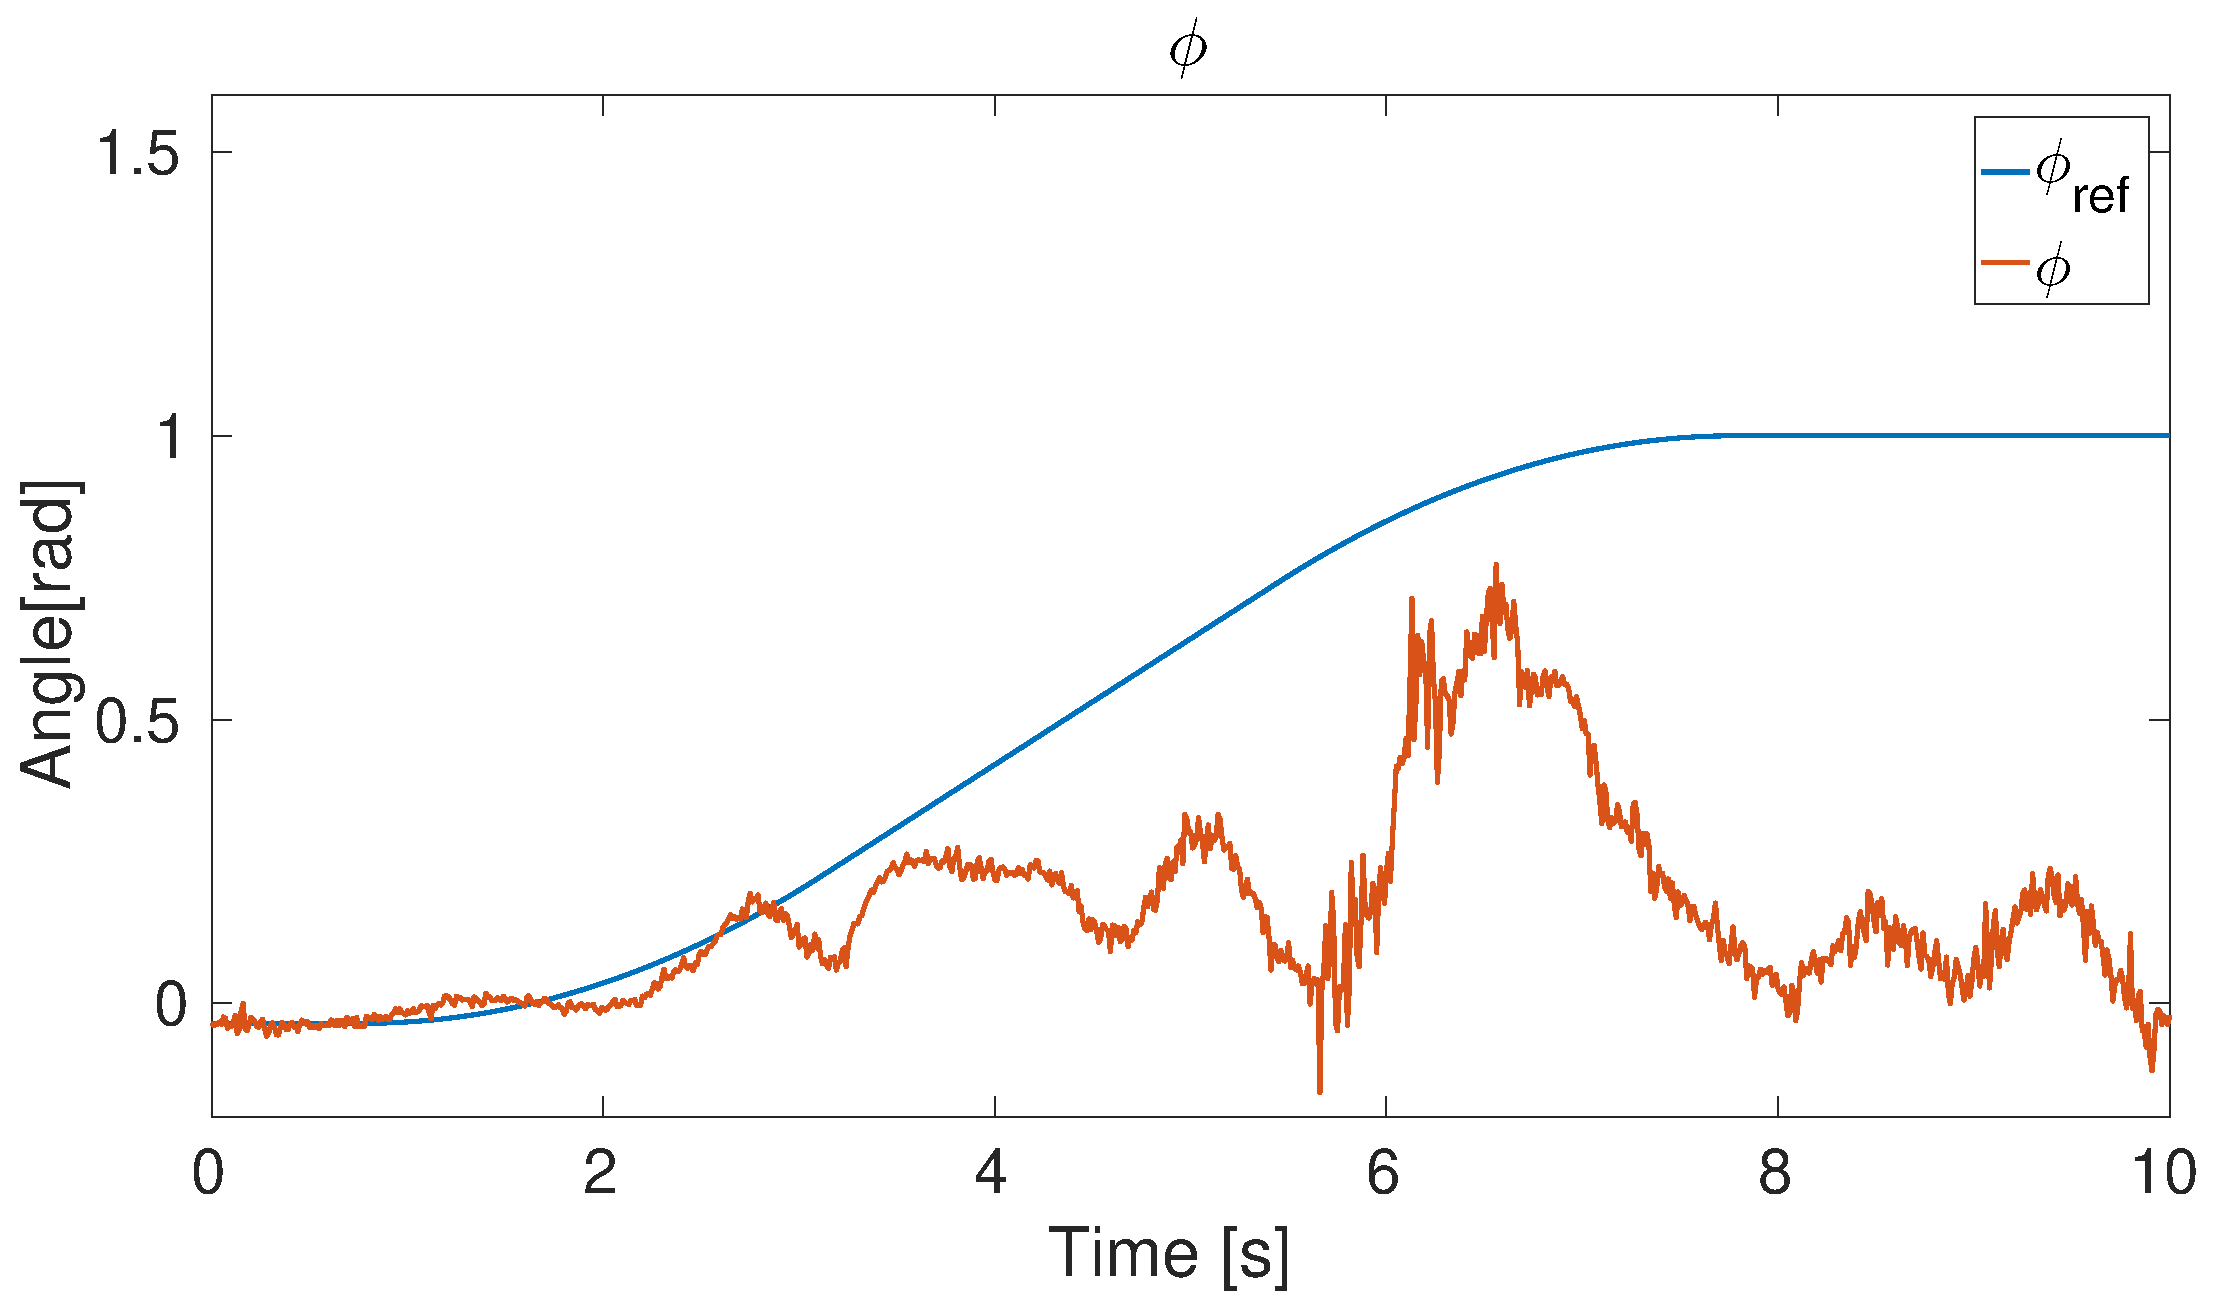
\includegraphics[width=0.4\textwidth]{testStepAllPhis3e10a1}}
  \qquad
  \subfloat[][\label{fig:simStepAllRollAttitude} Simulated response in $\rollAngle$.]{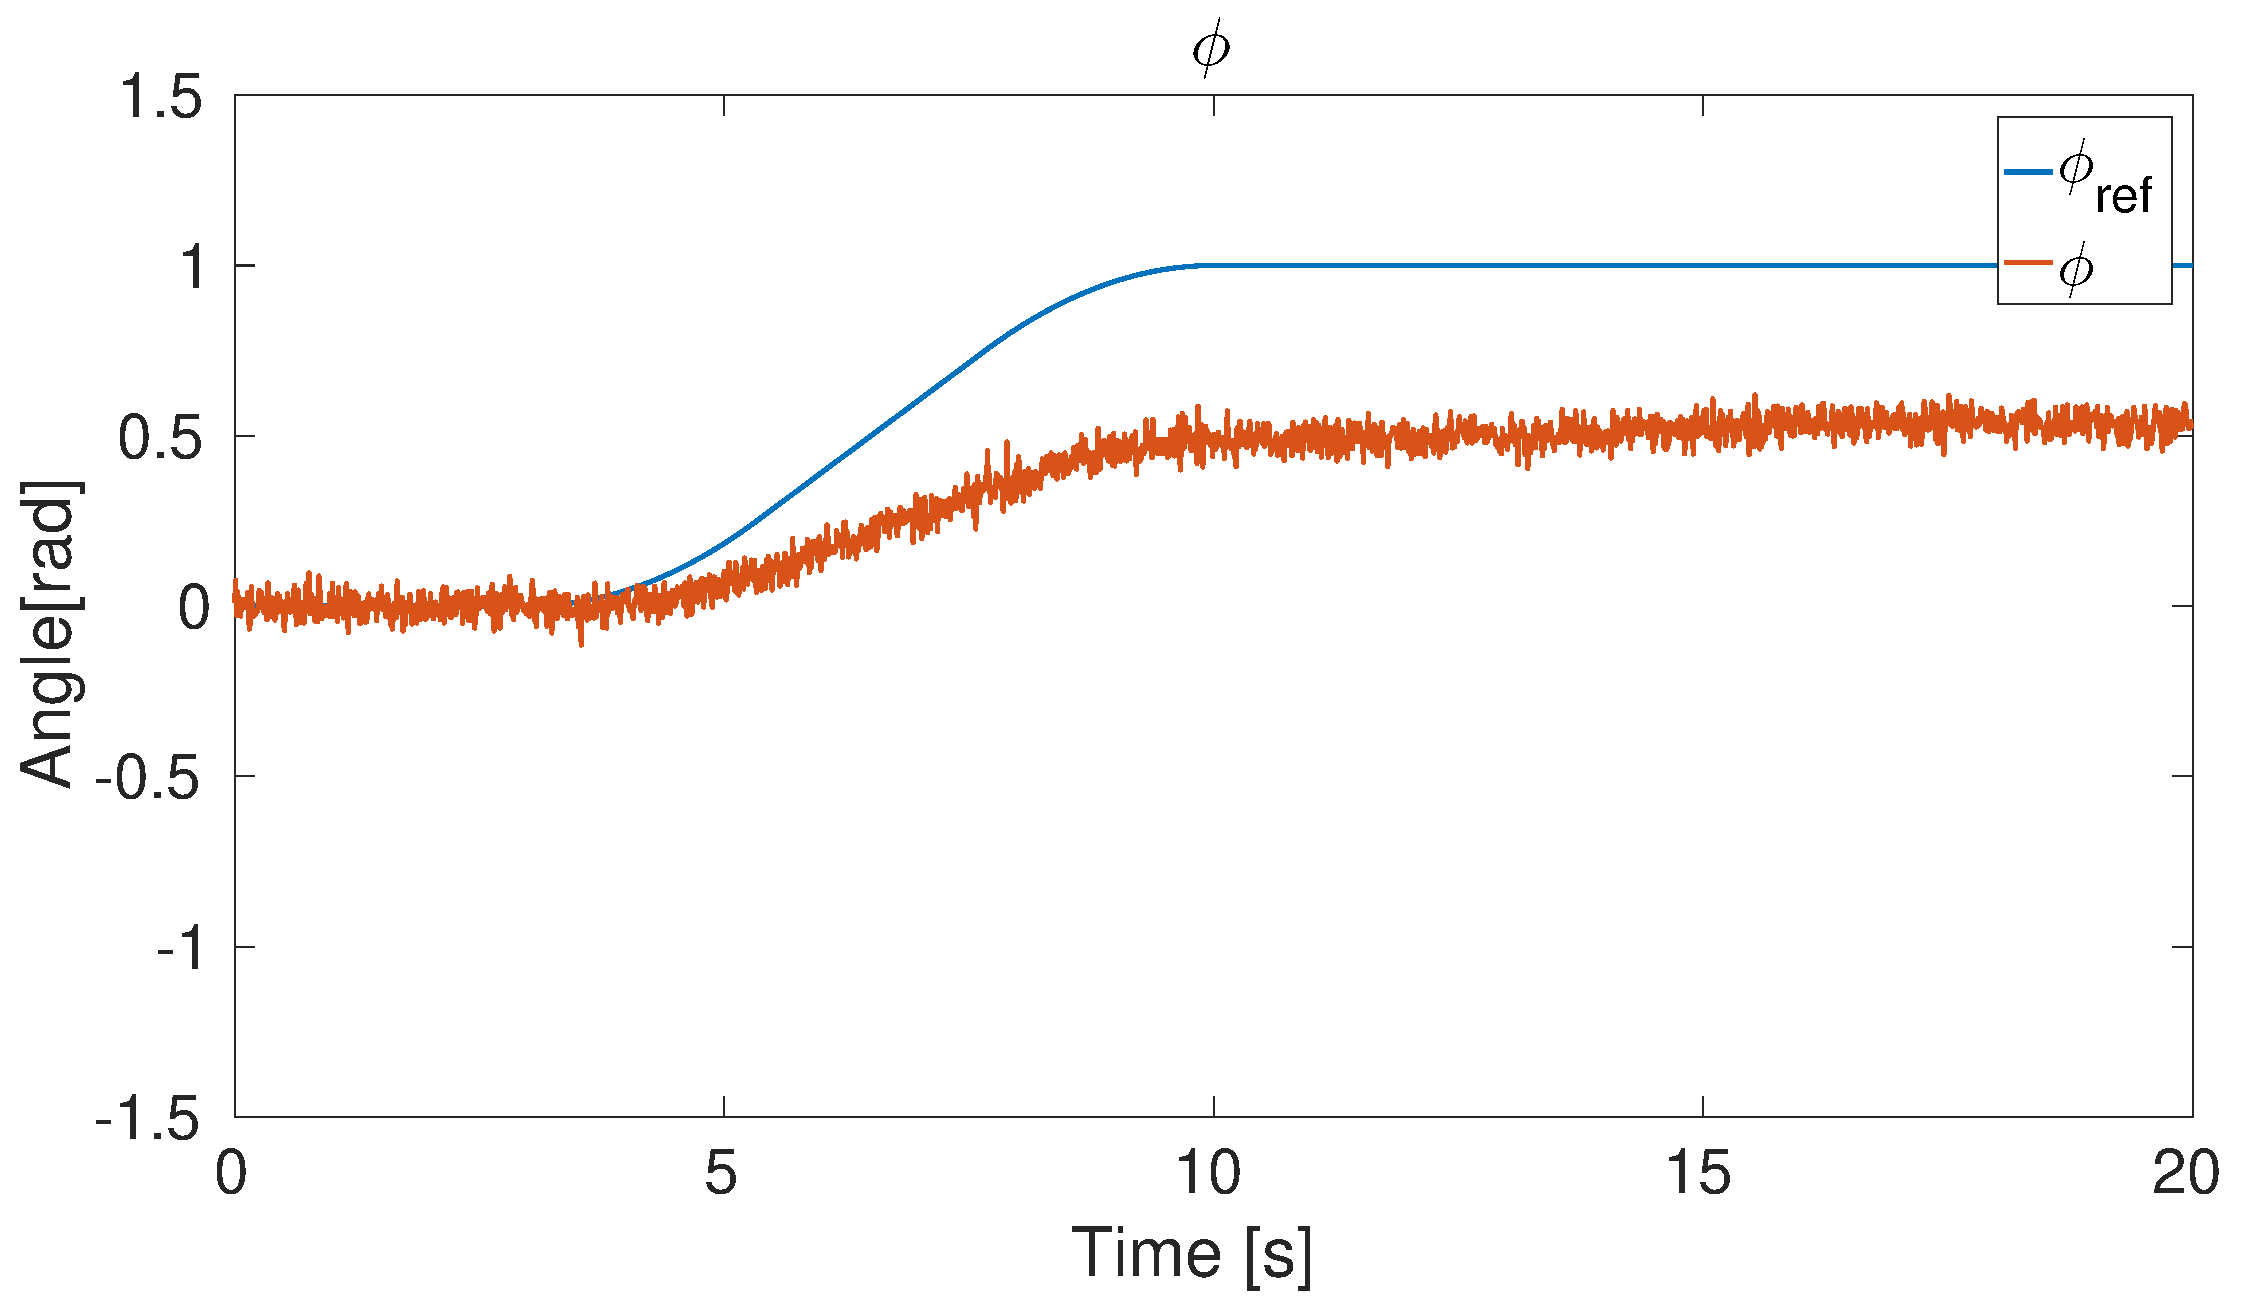
\includegraphics[width=0.4\textwidth]{simStepAllPhis3e10a1}}
  \qquad
  \subfloat[][\label{fig:TestStepAllPitchAttitude} Test response in $\pitchAngle$.]{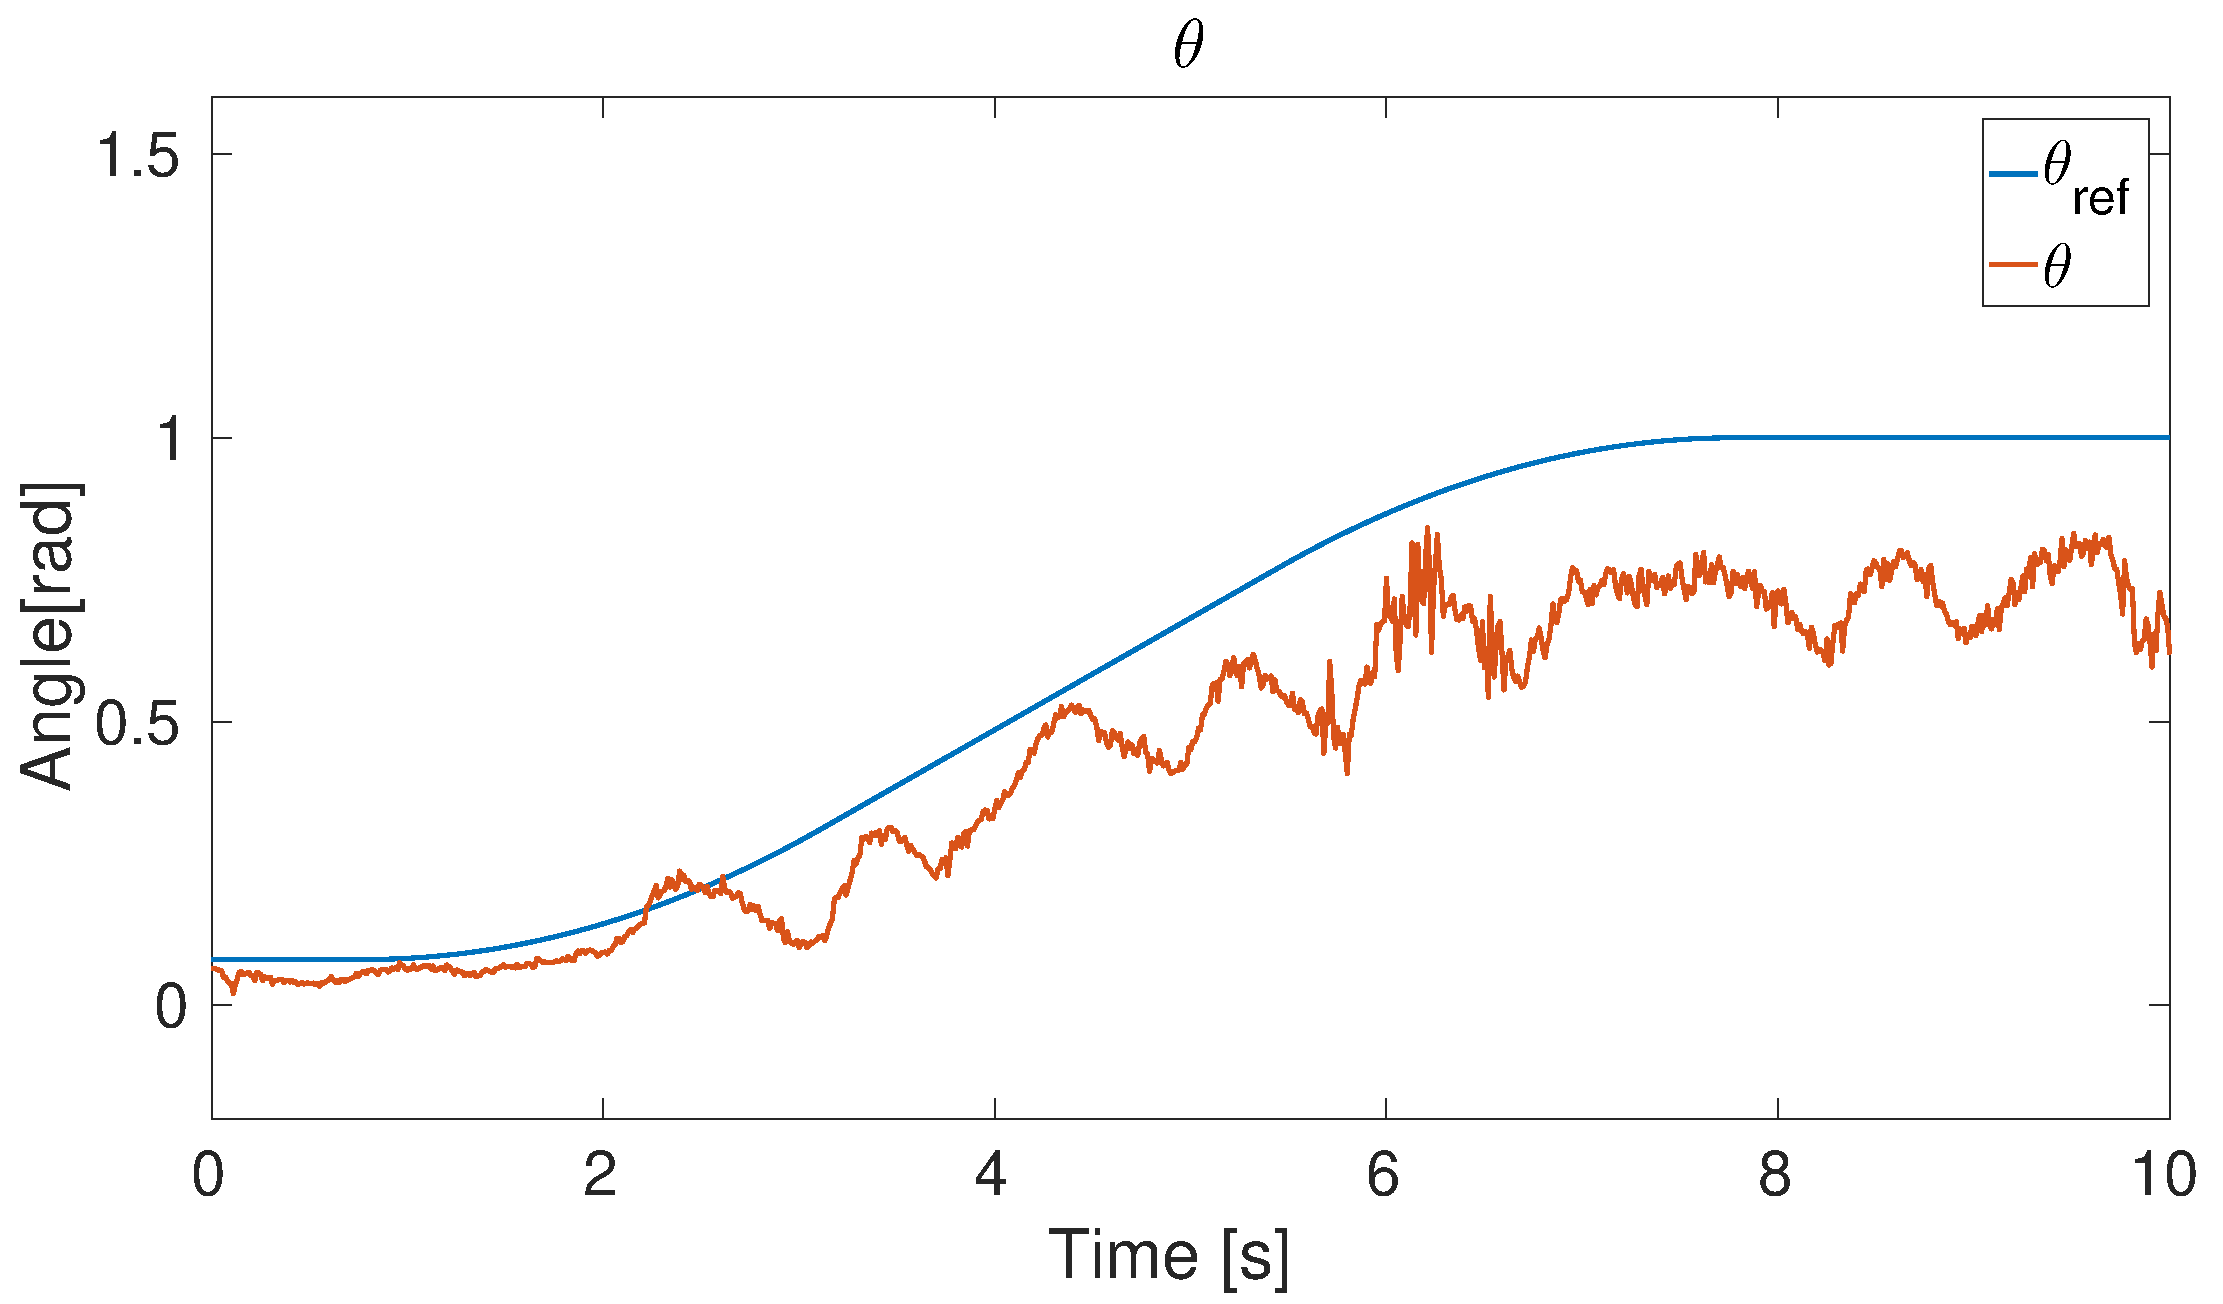
\includegraphics[width=0.4\textwidth]{testStepAllThetas3e10a1}}
  \qquad
  \subfloat[][\label{fig:simStepAllPitchAttitude} Simulated response in $\pitchAngle$.]{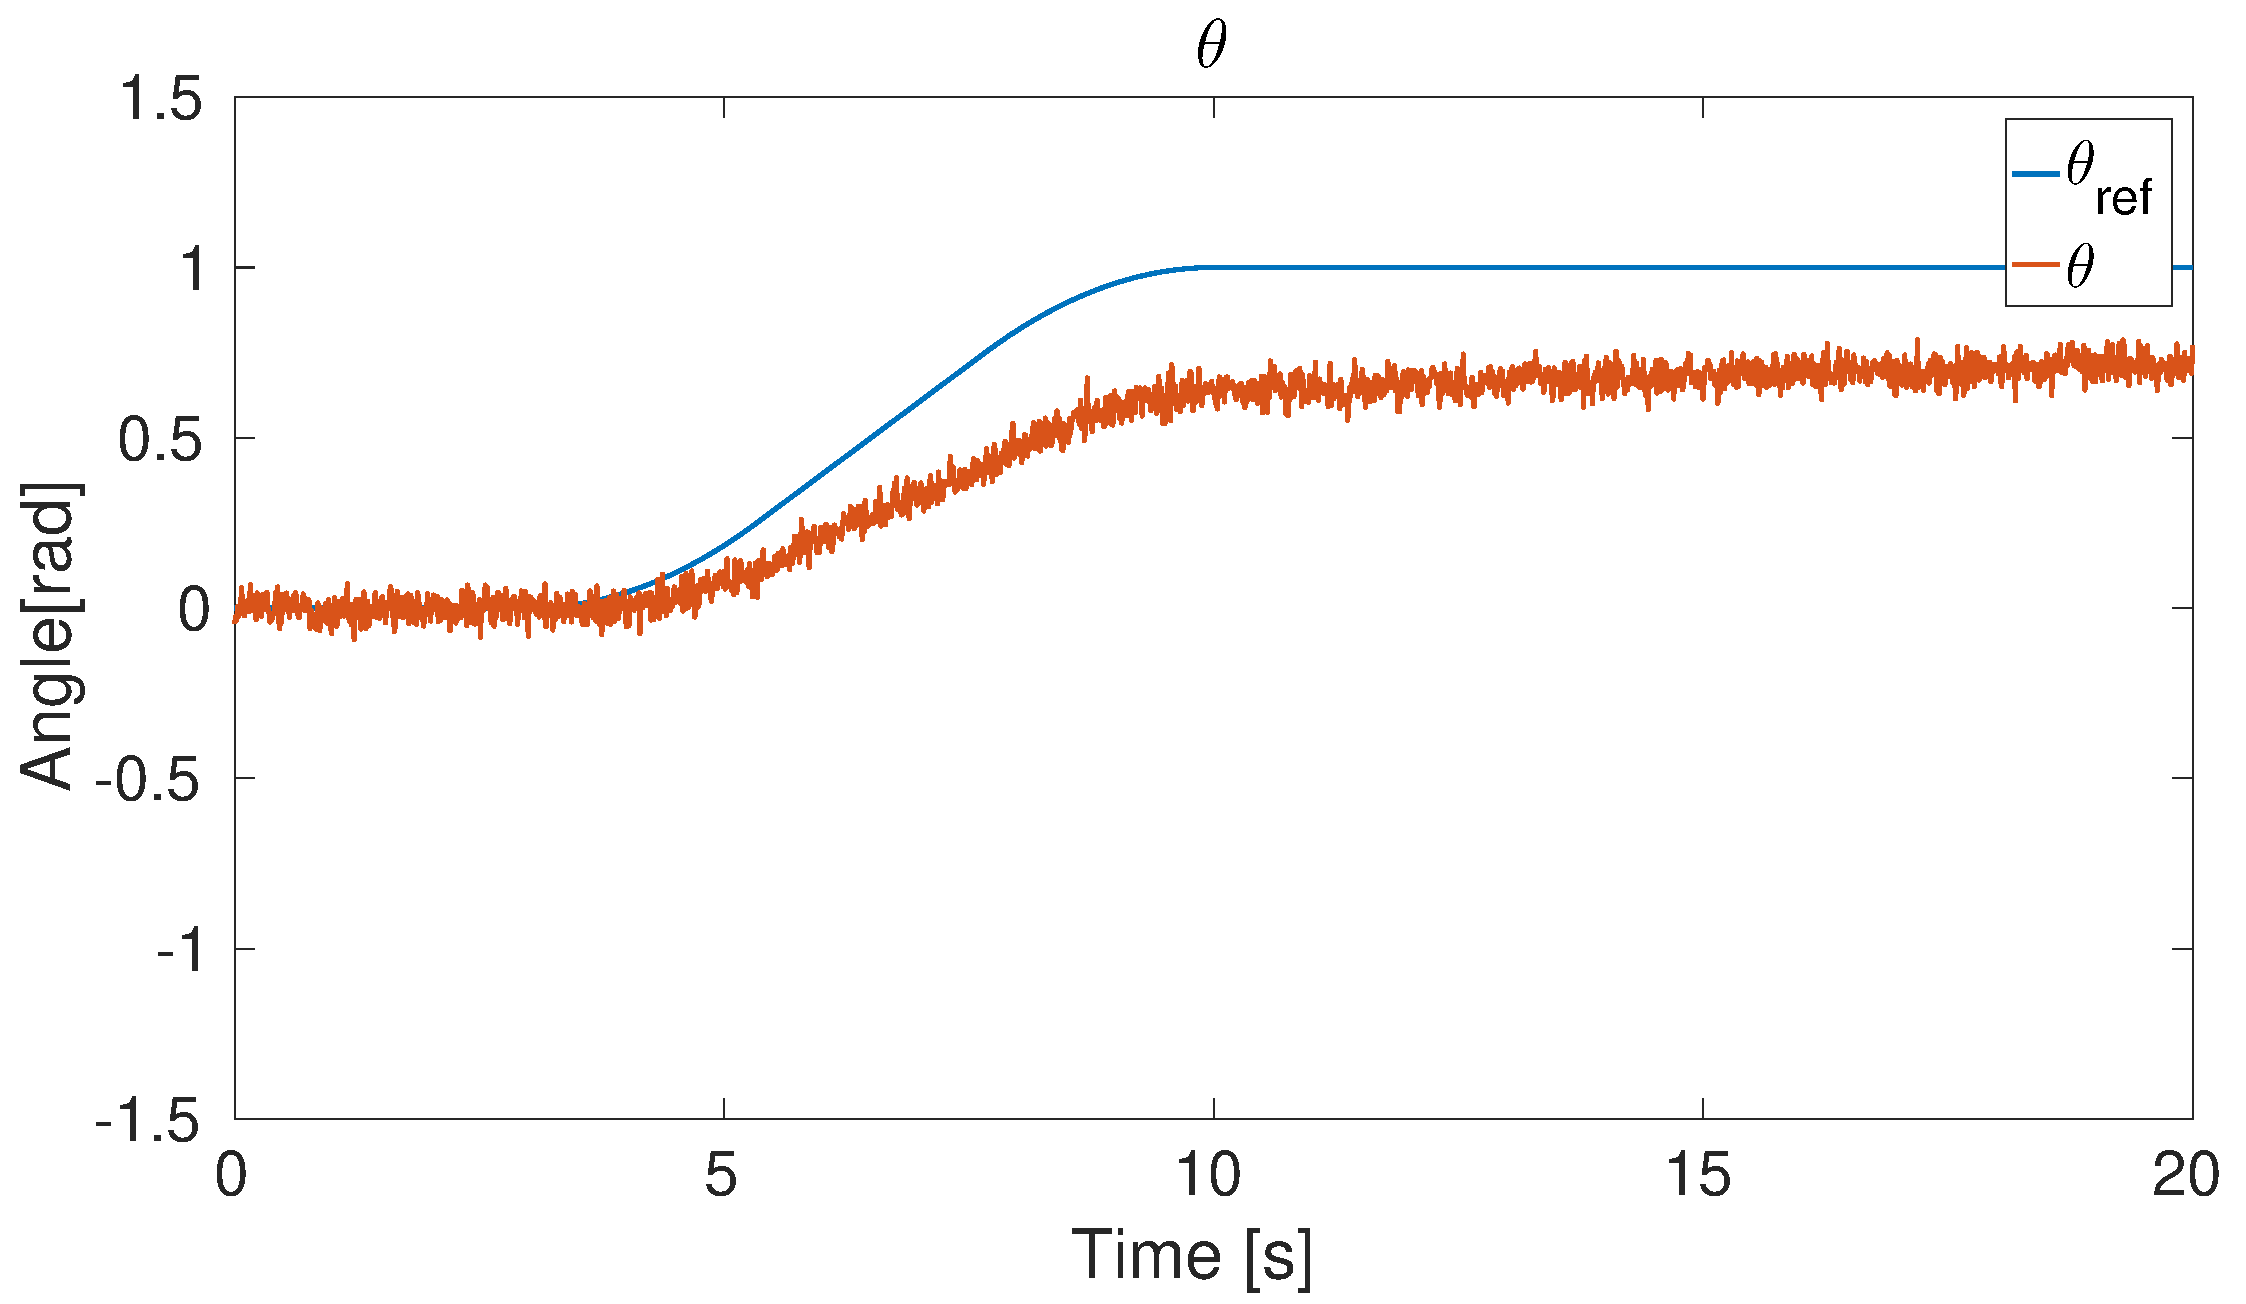
\includegraphics[width=0.4\textwidth]{simStepAllThetas3e10a1}}
  \qquad
  \subfloat[][\label{fig:TestStepAllYawAttitude} Test response in $\yawAngle$.]{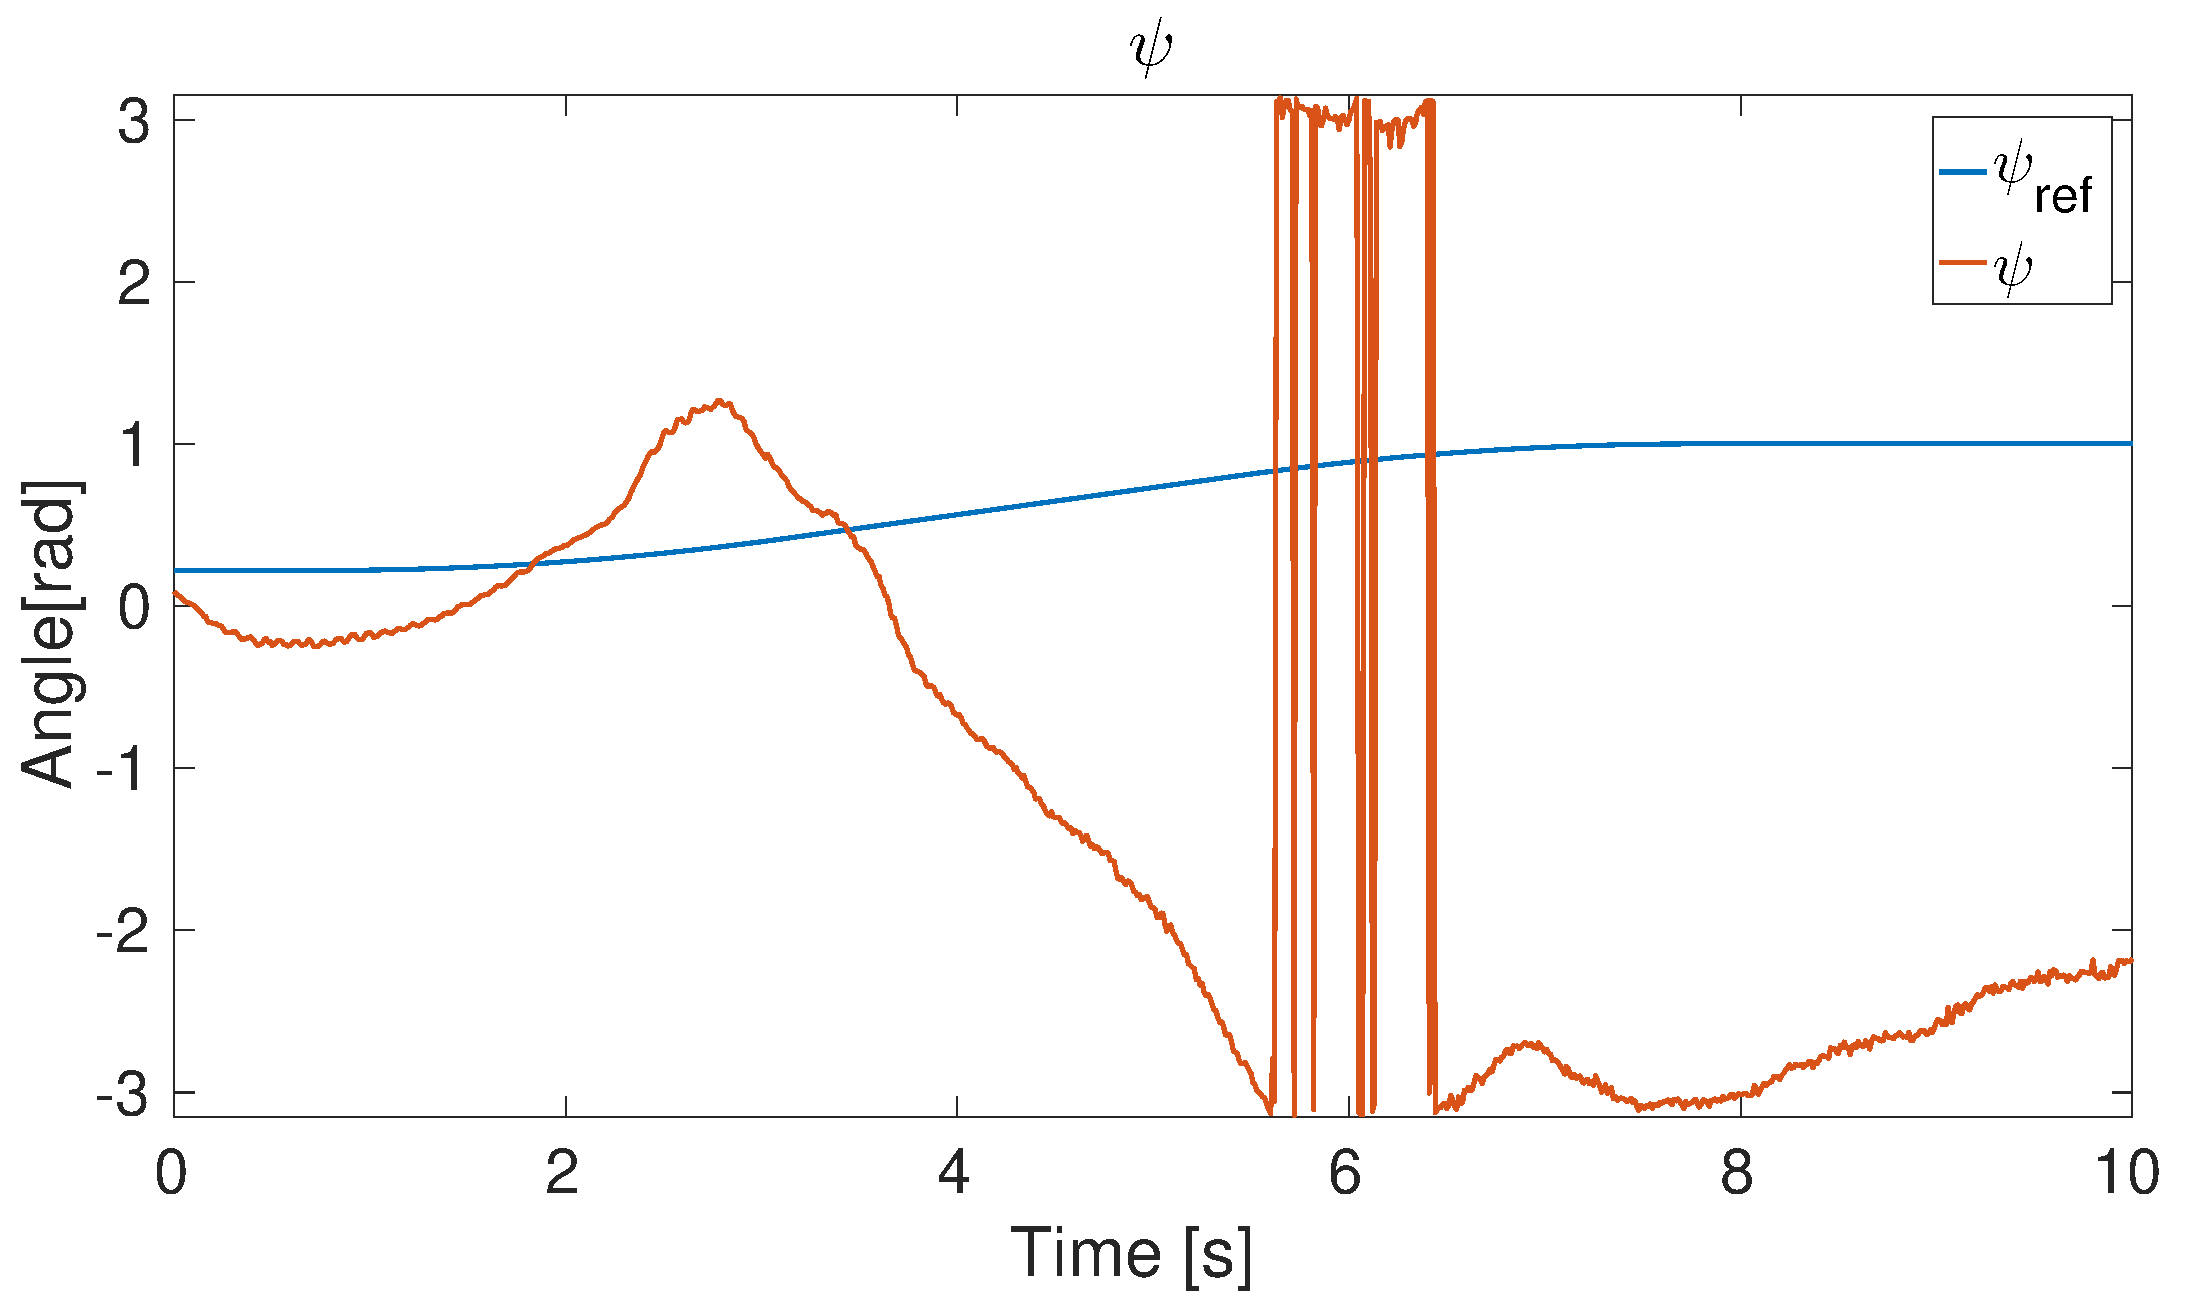
\includegraphics[width=0.4\textwidth]{testStepAllPsis3e10a1}}
  \qquad
  \subfloat[][\label{fig:simStepAllYawAttitude} Simulated response in $\yawAngle$.]{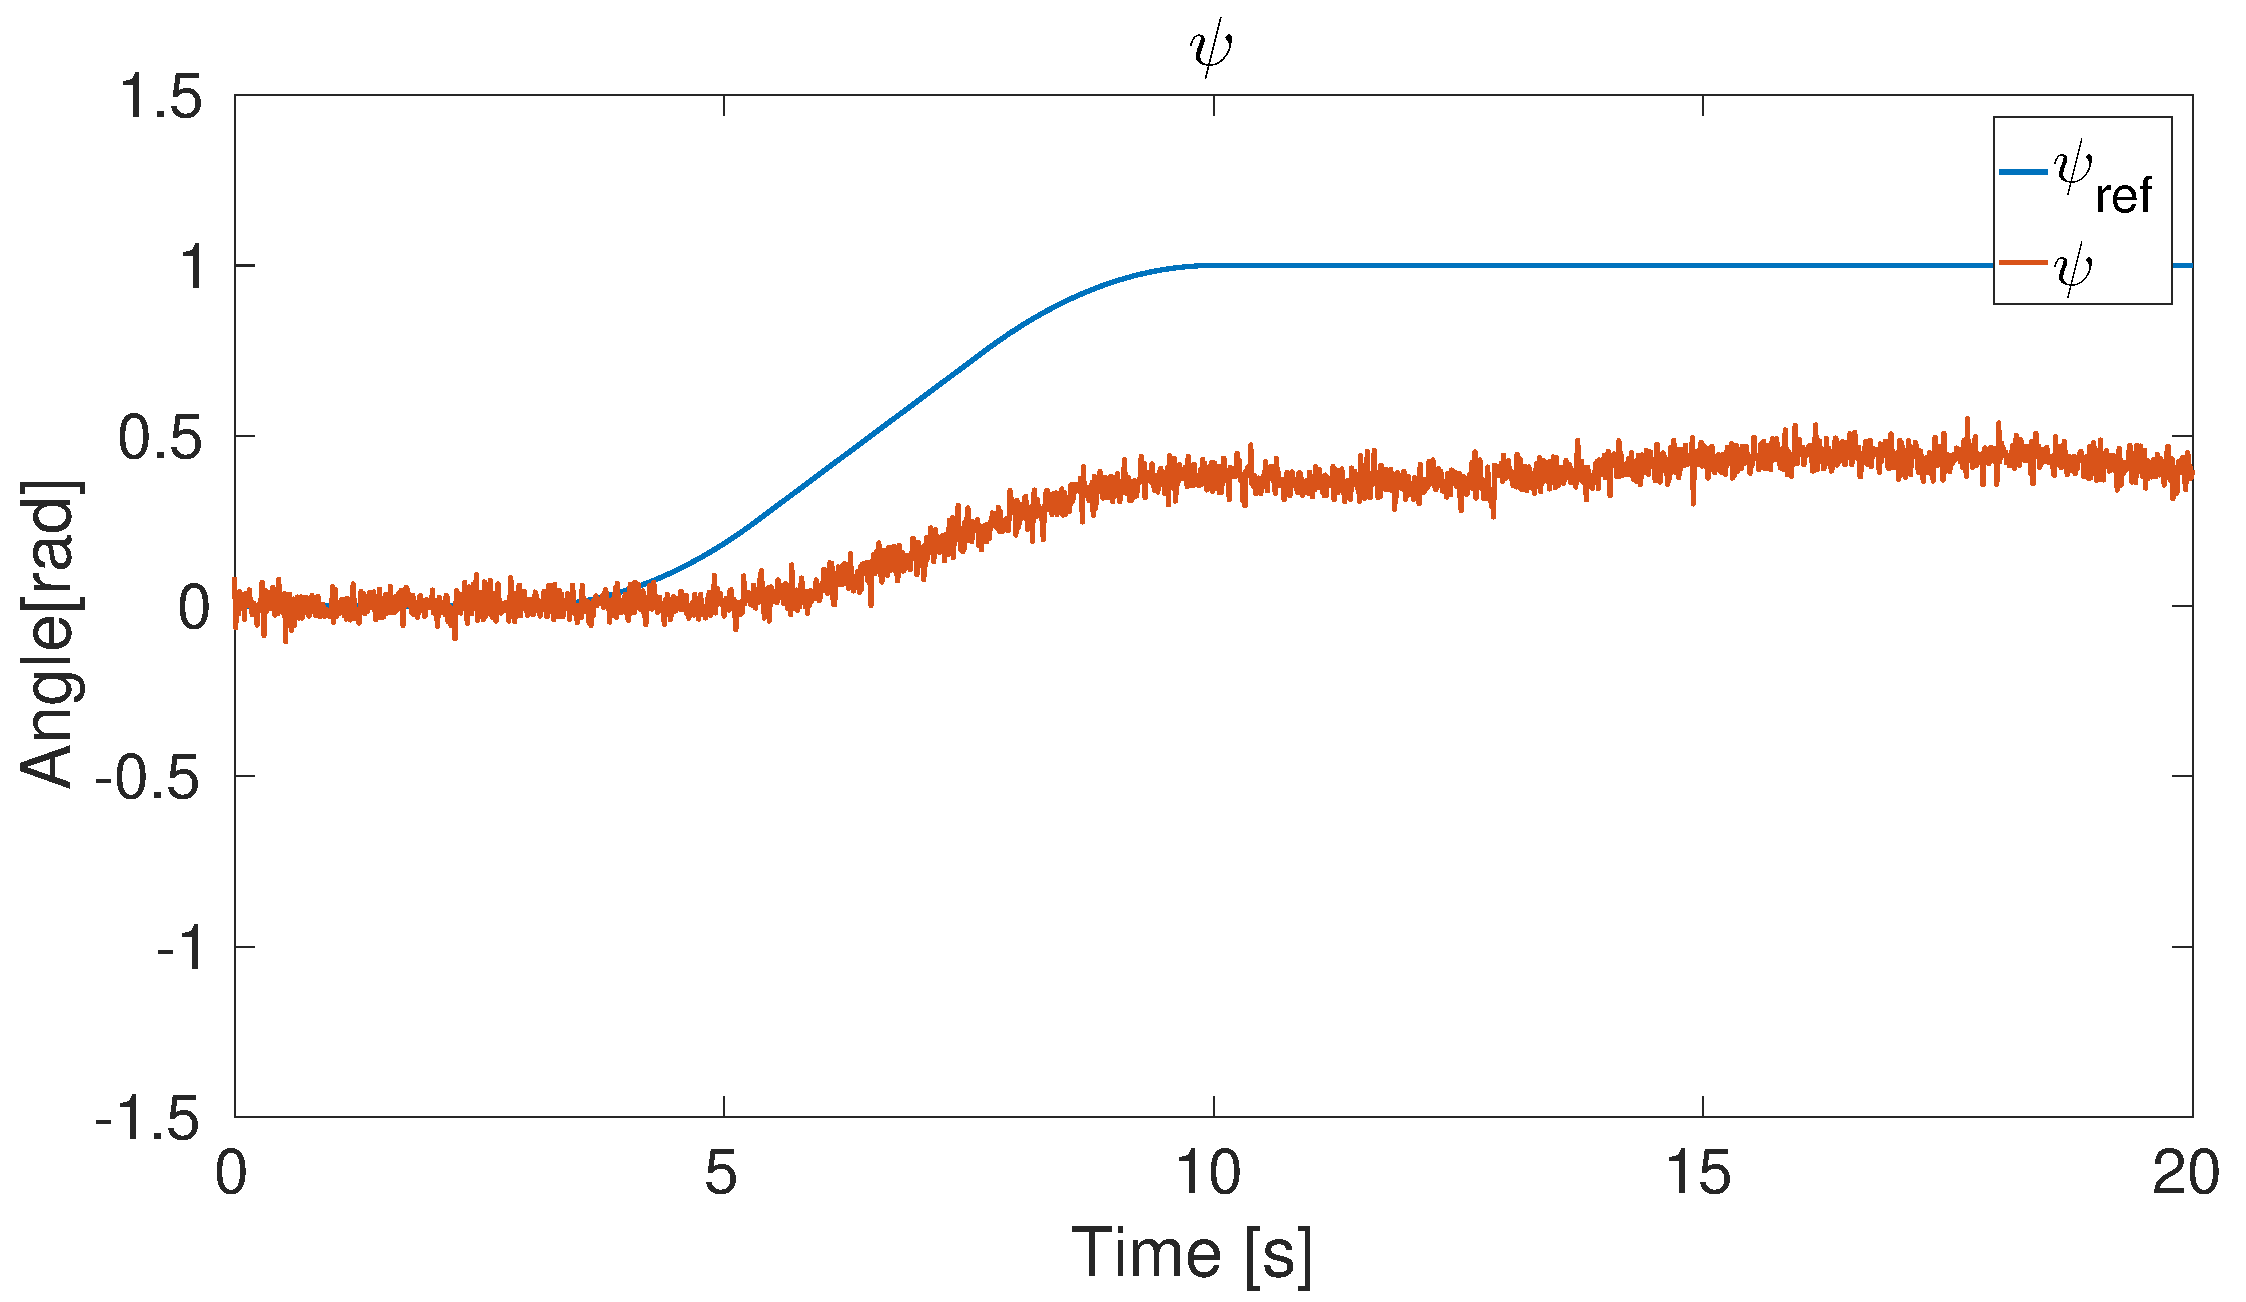
\includegraphics[width=0.4\textwidth]{simStepAllPsis3e10a1}}
  \caption{\label{fig:StepAllAttitude}% 
 A smooth step with $q_{\text{0}} = 0$, $q_{\text{f}} = 1$, $t_{\text{s}} = 3$, $t_{\text{f}} = 15$ and $V = 1.5 (q_{\text{f}} - q_{\text{0}})/(t_{\text{f}} - t_{\text{s}}))$ was applied in all attitude angles at the same time while using the attitude controller.}
\end{figure}

\Figureref{fig:StepAllAttitude} shows the smooth-step reference signals applied in all attitude angles while using the attitude controller without linearisation. Initially, the roll and pitch angle did not follow the reference signals. During field tests, the roll angle was oscillative and had a steady-state error of $0.9$. However, the control of the pitch angle was objectively better, with a steady-state error of $0.4$. The yaw angle could not be stabilised during the field test and drifted throughout the tests. The attitude angles did not reach the reference signals in the simulated test case either. The pitch angle had a steady-state error of $0.3$ while the other angles had a steady-state error of $0.5$.

\begin{figure}
\centering
  \subfloat[][\label{fig:testSinAllRollAttitude} Test response in $\rollAngle$.]{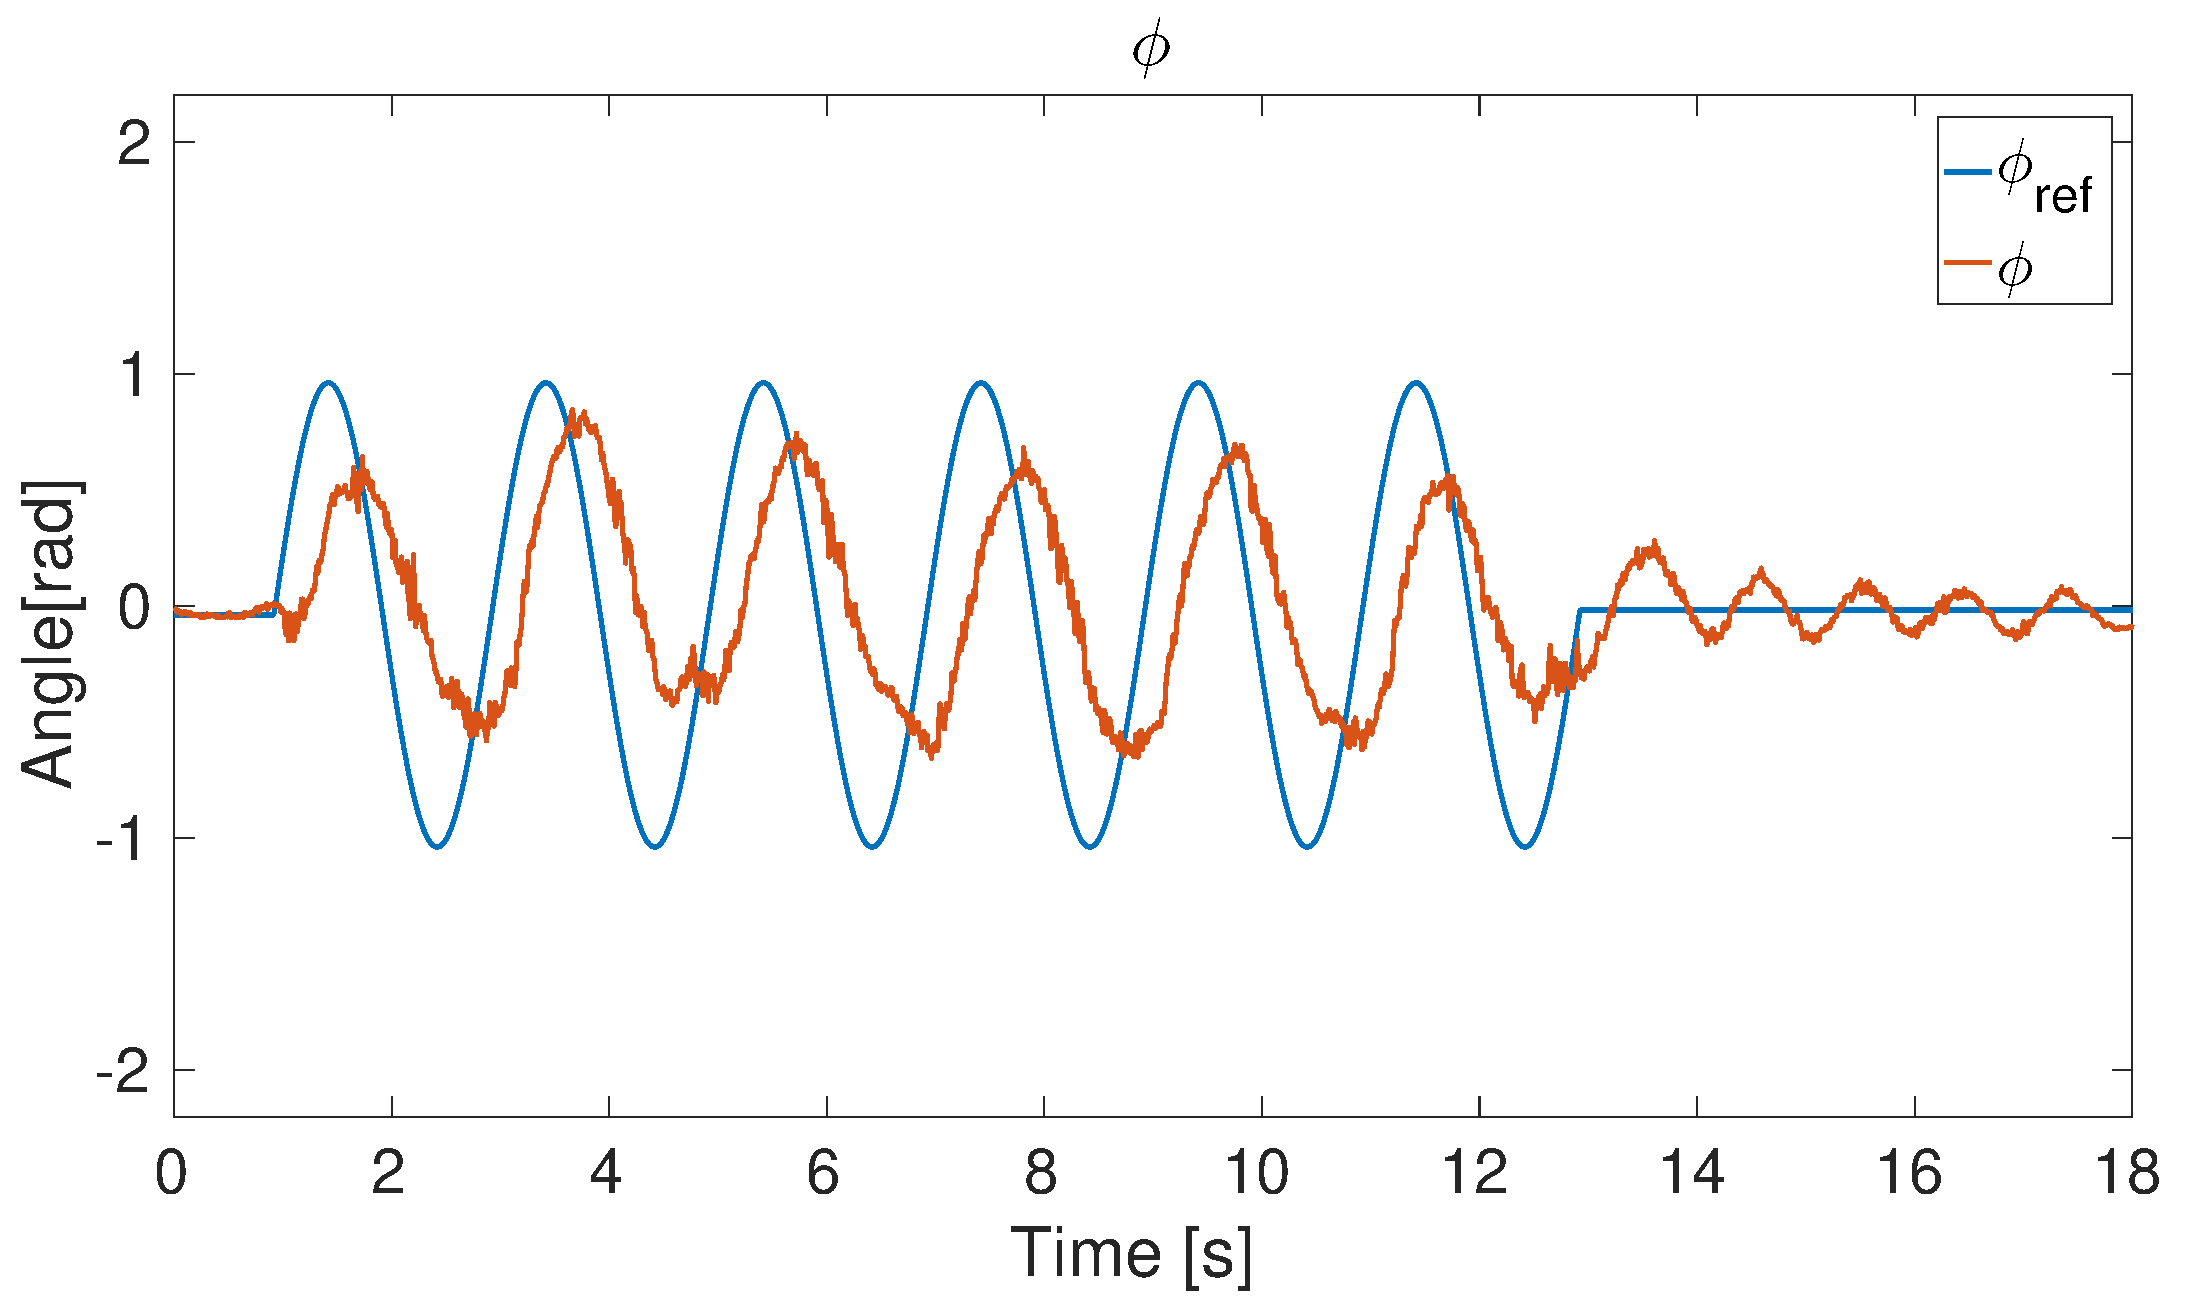
\includegraphics[width=0.4\textwidth]{testSinAllPhiA1}}
  \qquad
  \subfloat[][\label{fig:simSinAllRollAttitude} Simulated response in $\rollAngle$.]{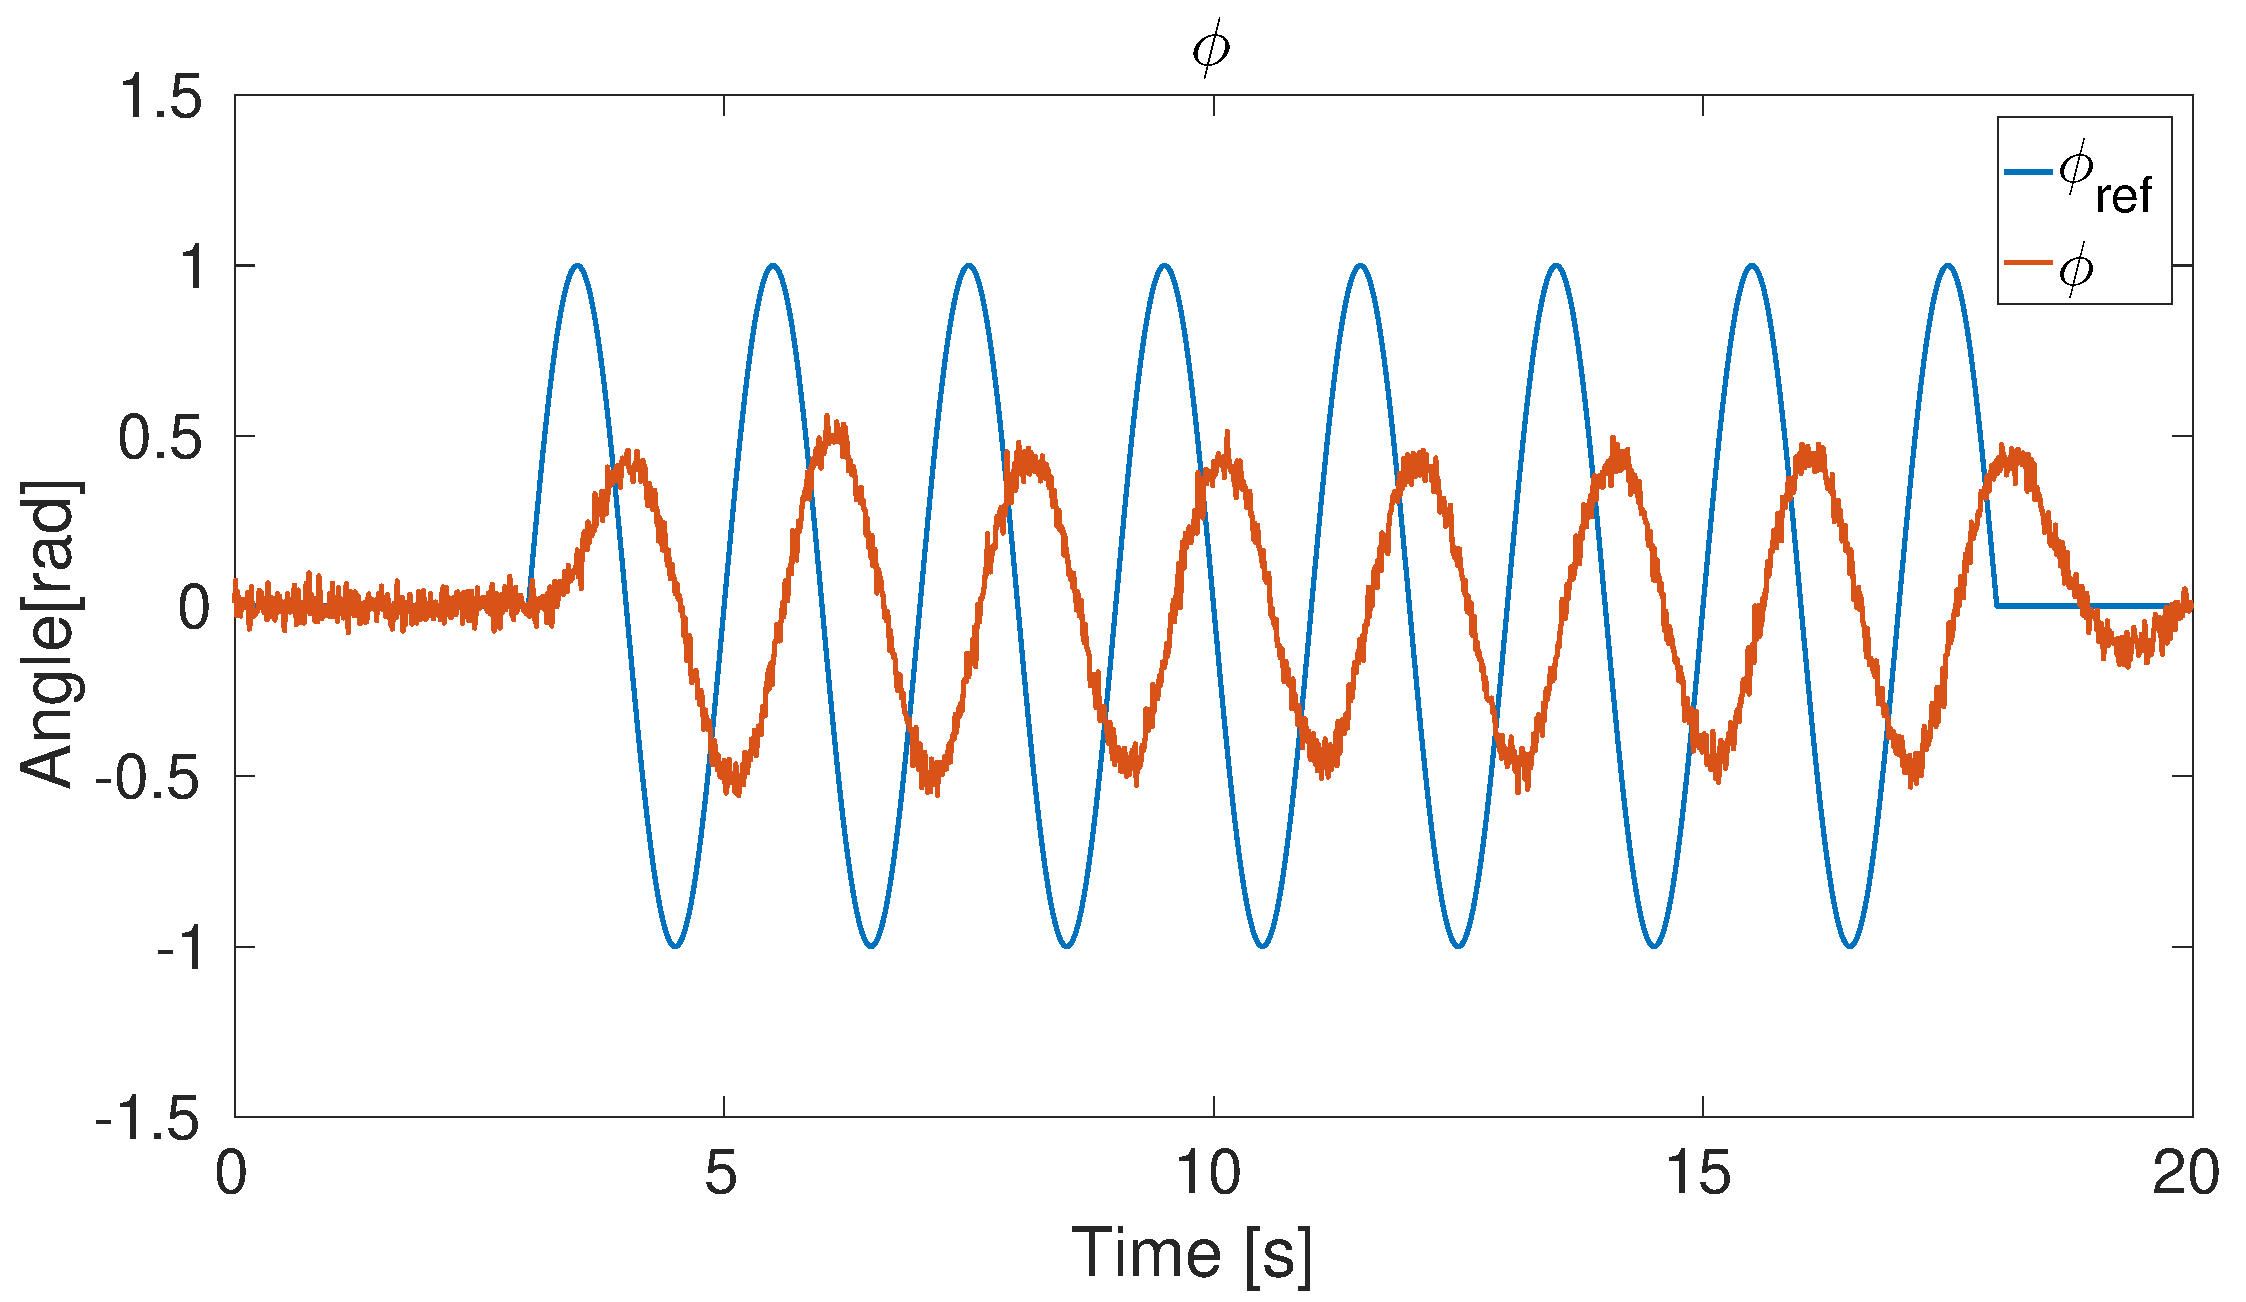
\includegraphics[width=0.4\textwidth]{simSinAllPhiA1}}
  \qquad
  \subfloat[][\label{fig:testSinAllPitchAttitude} Test response in $\pitchAngle$.]{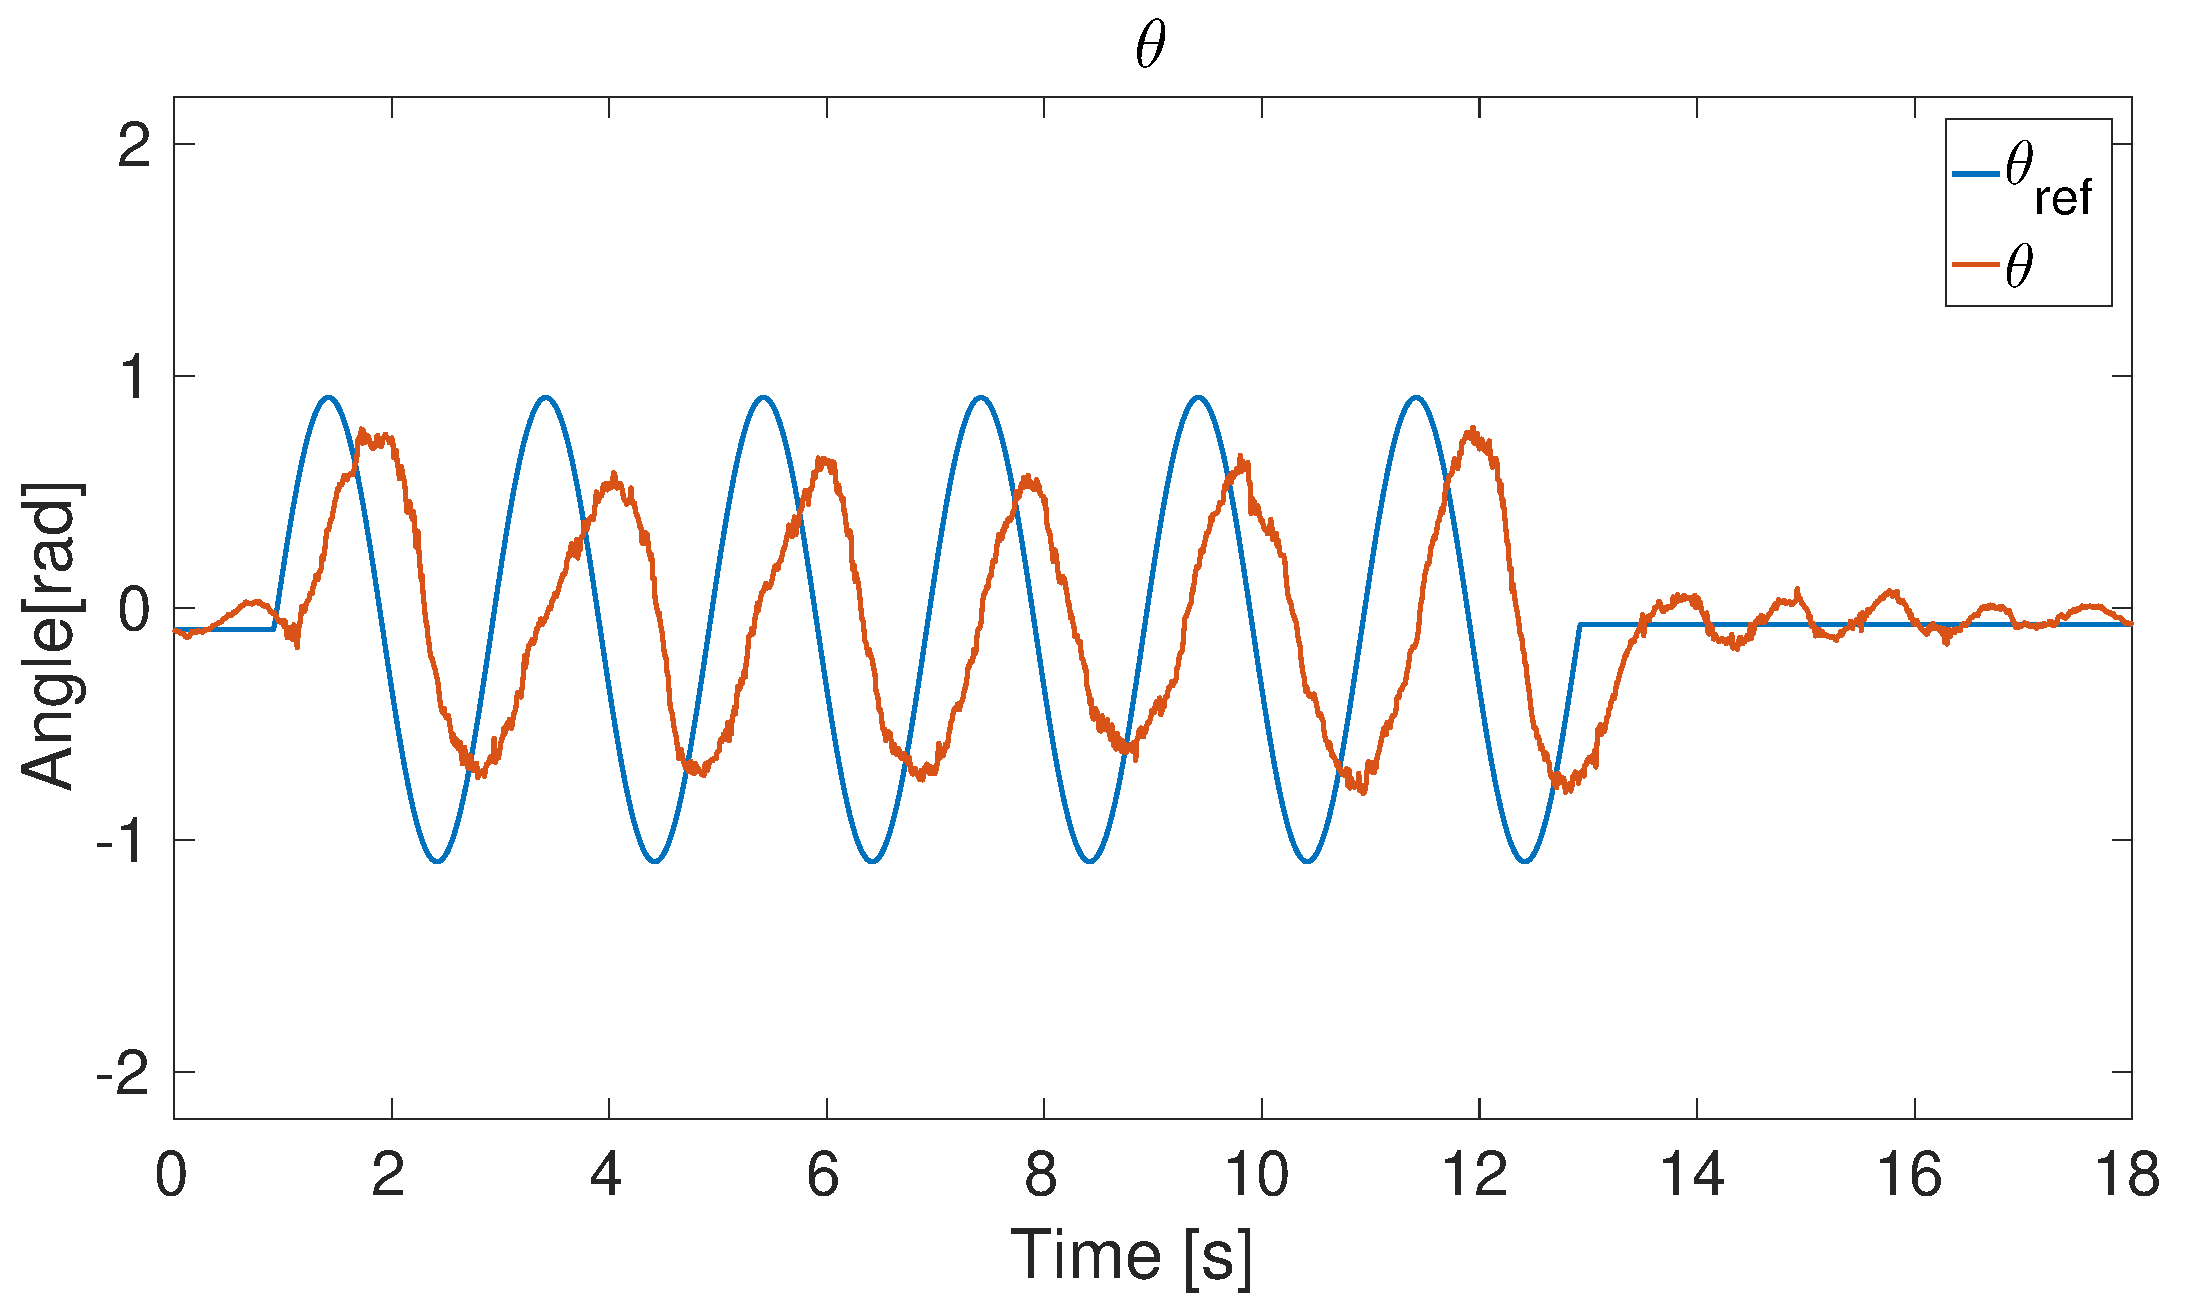
\includegraphics[width=0.4\textwidth]{testSinAllThetaA1}}
  \qquad
  \subfloat[][\label{fig:simSinAllPitchAttitude} Simulated response in $\pitchAngle$.]{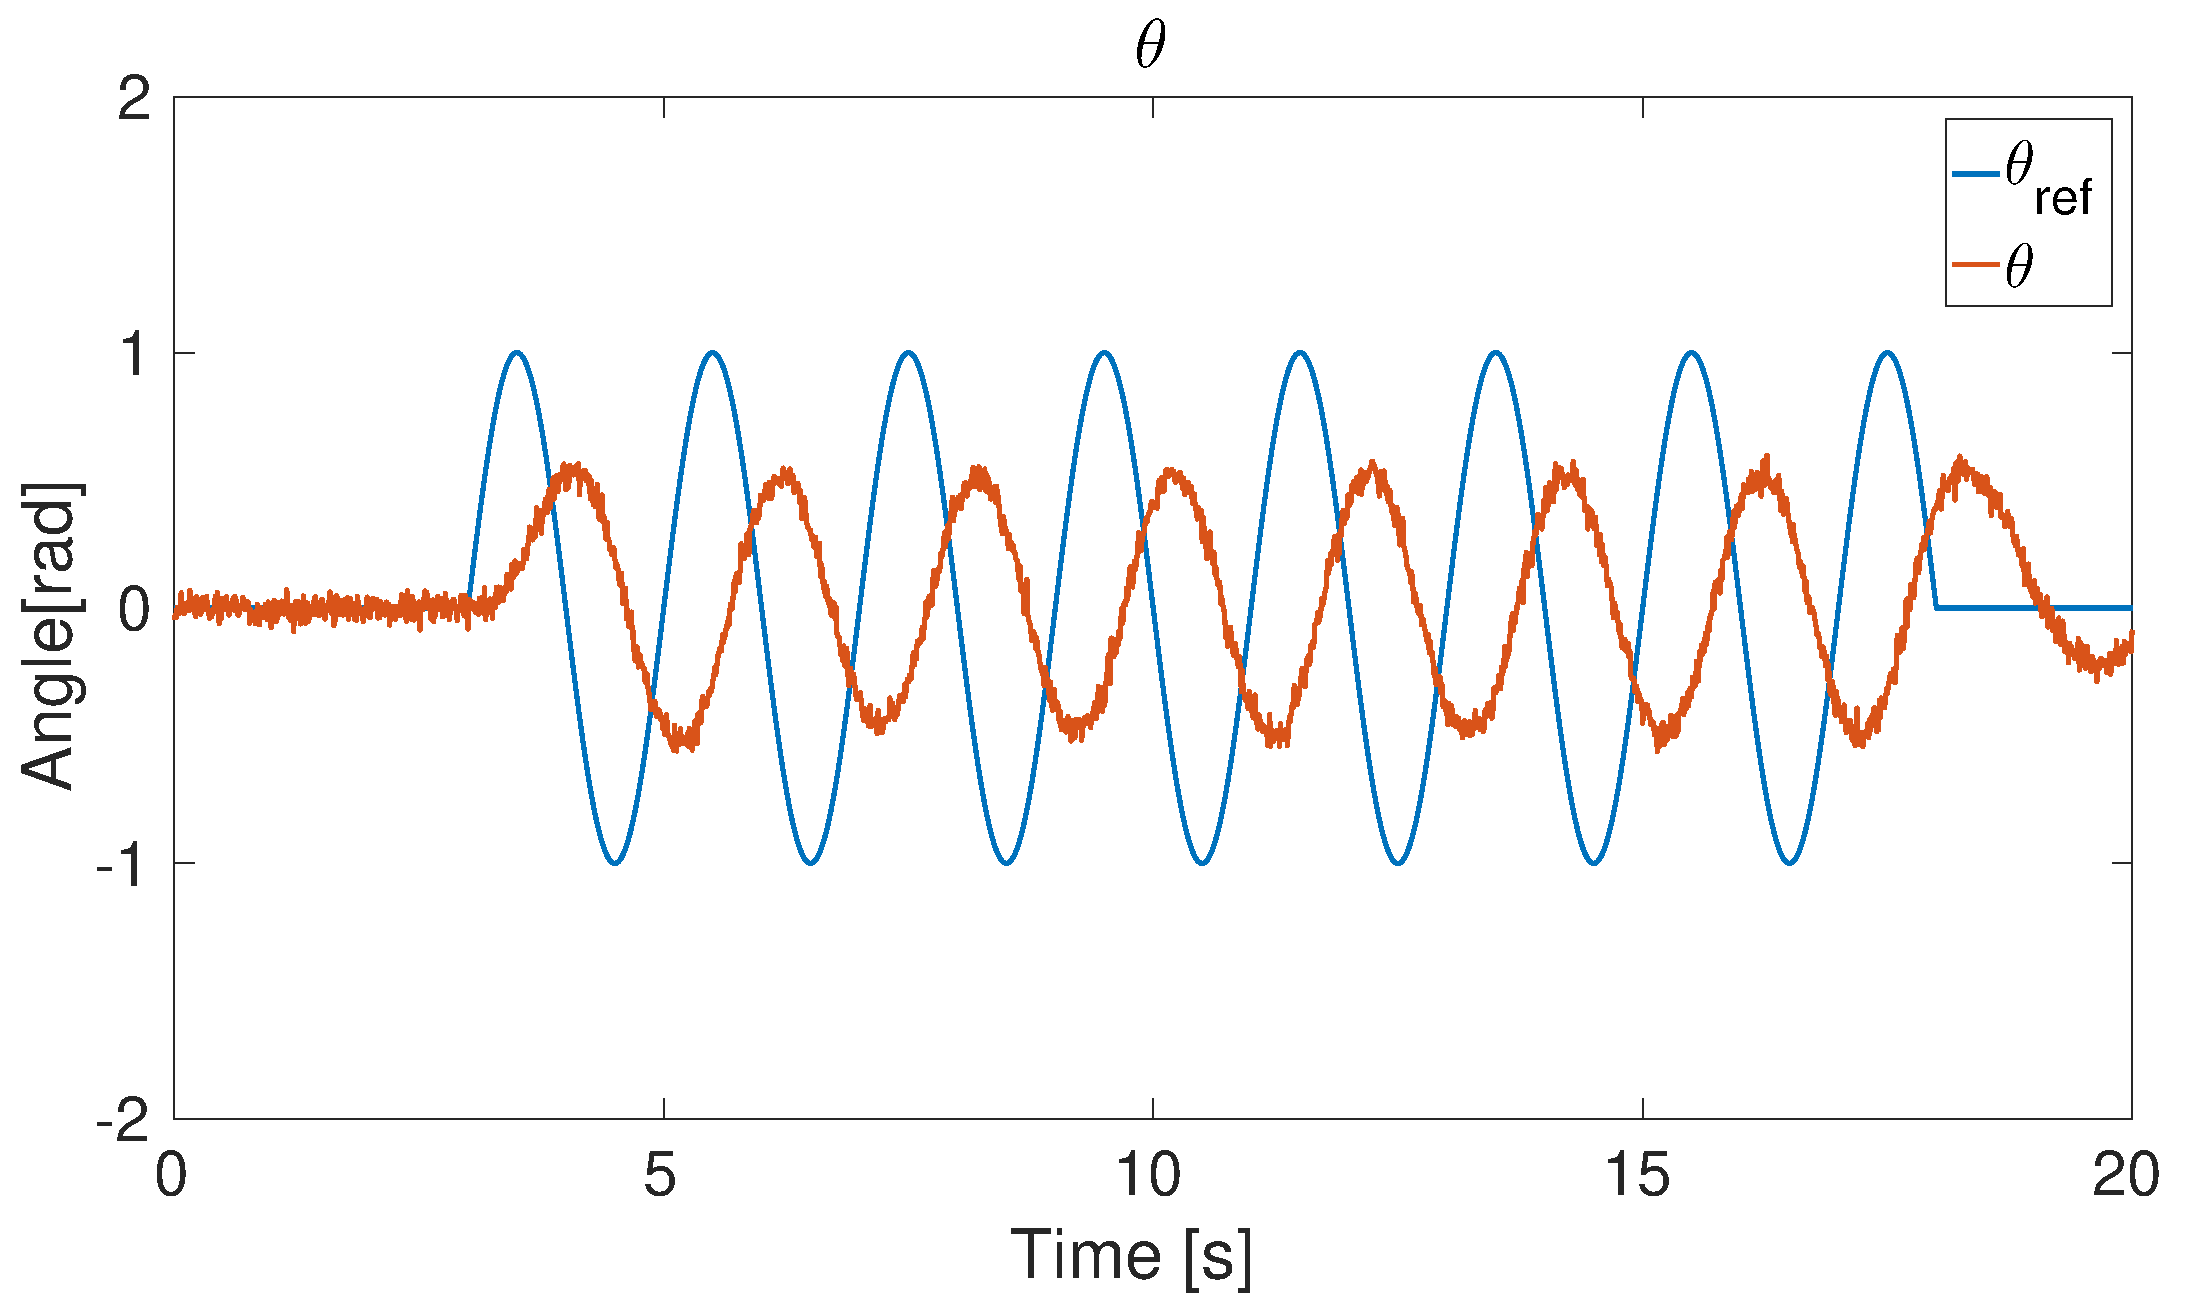
\includegraphics[width=0.4\textwidth]{simSinAllThetaA1}}
  \qquad
  \subfloat[][\label{fig:testSinAllYawAttitude} Test response in $\yawAngle$.]{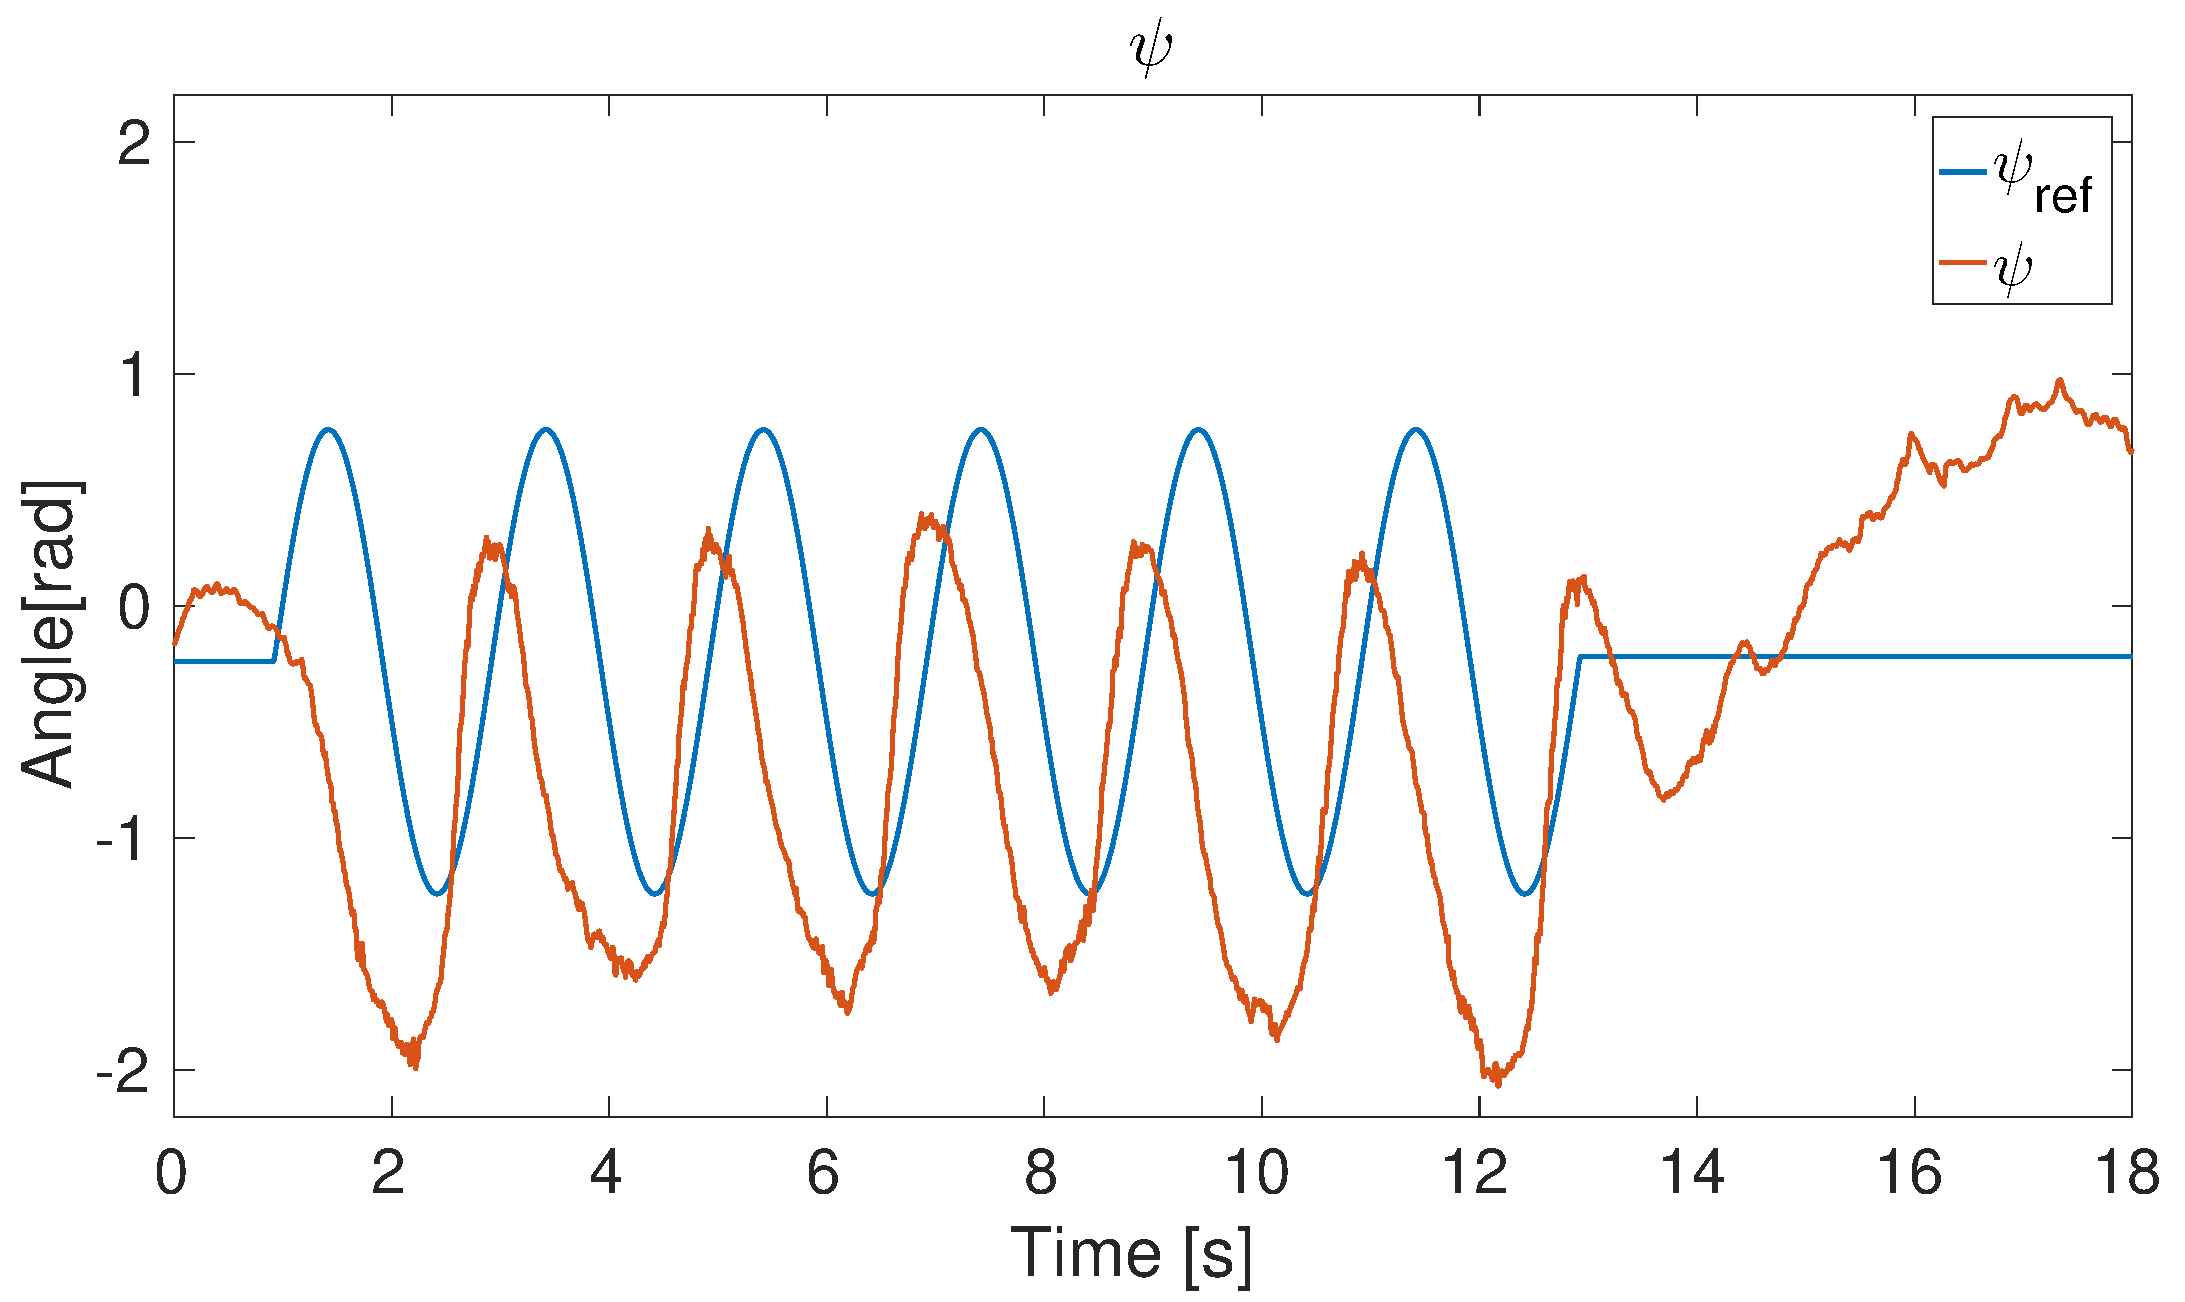
\includegraphics[width=0.4\textwidth]{testSinAllPsiA1}}
  \qquad
  \subfloat[][\label{fig:simSinAllYawAttitude} Simulated response in $\yawAngle$.]{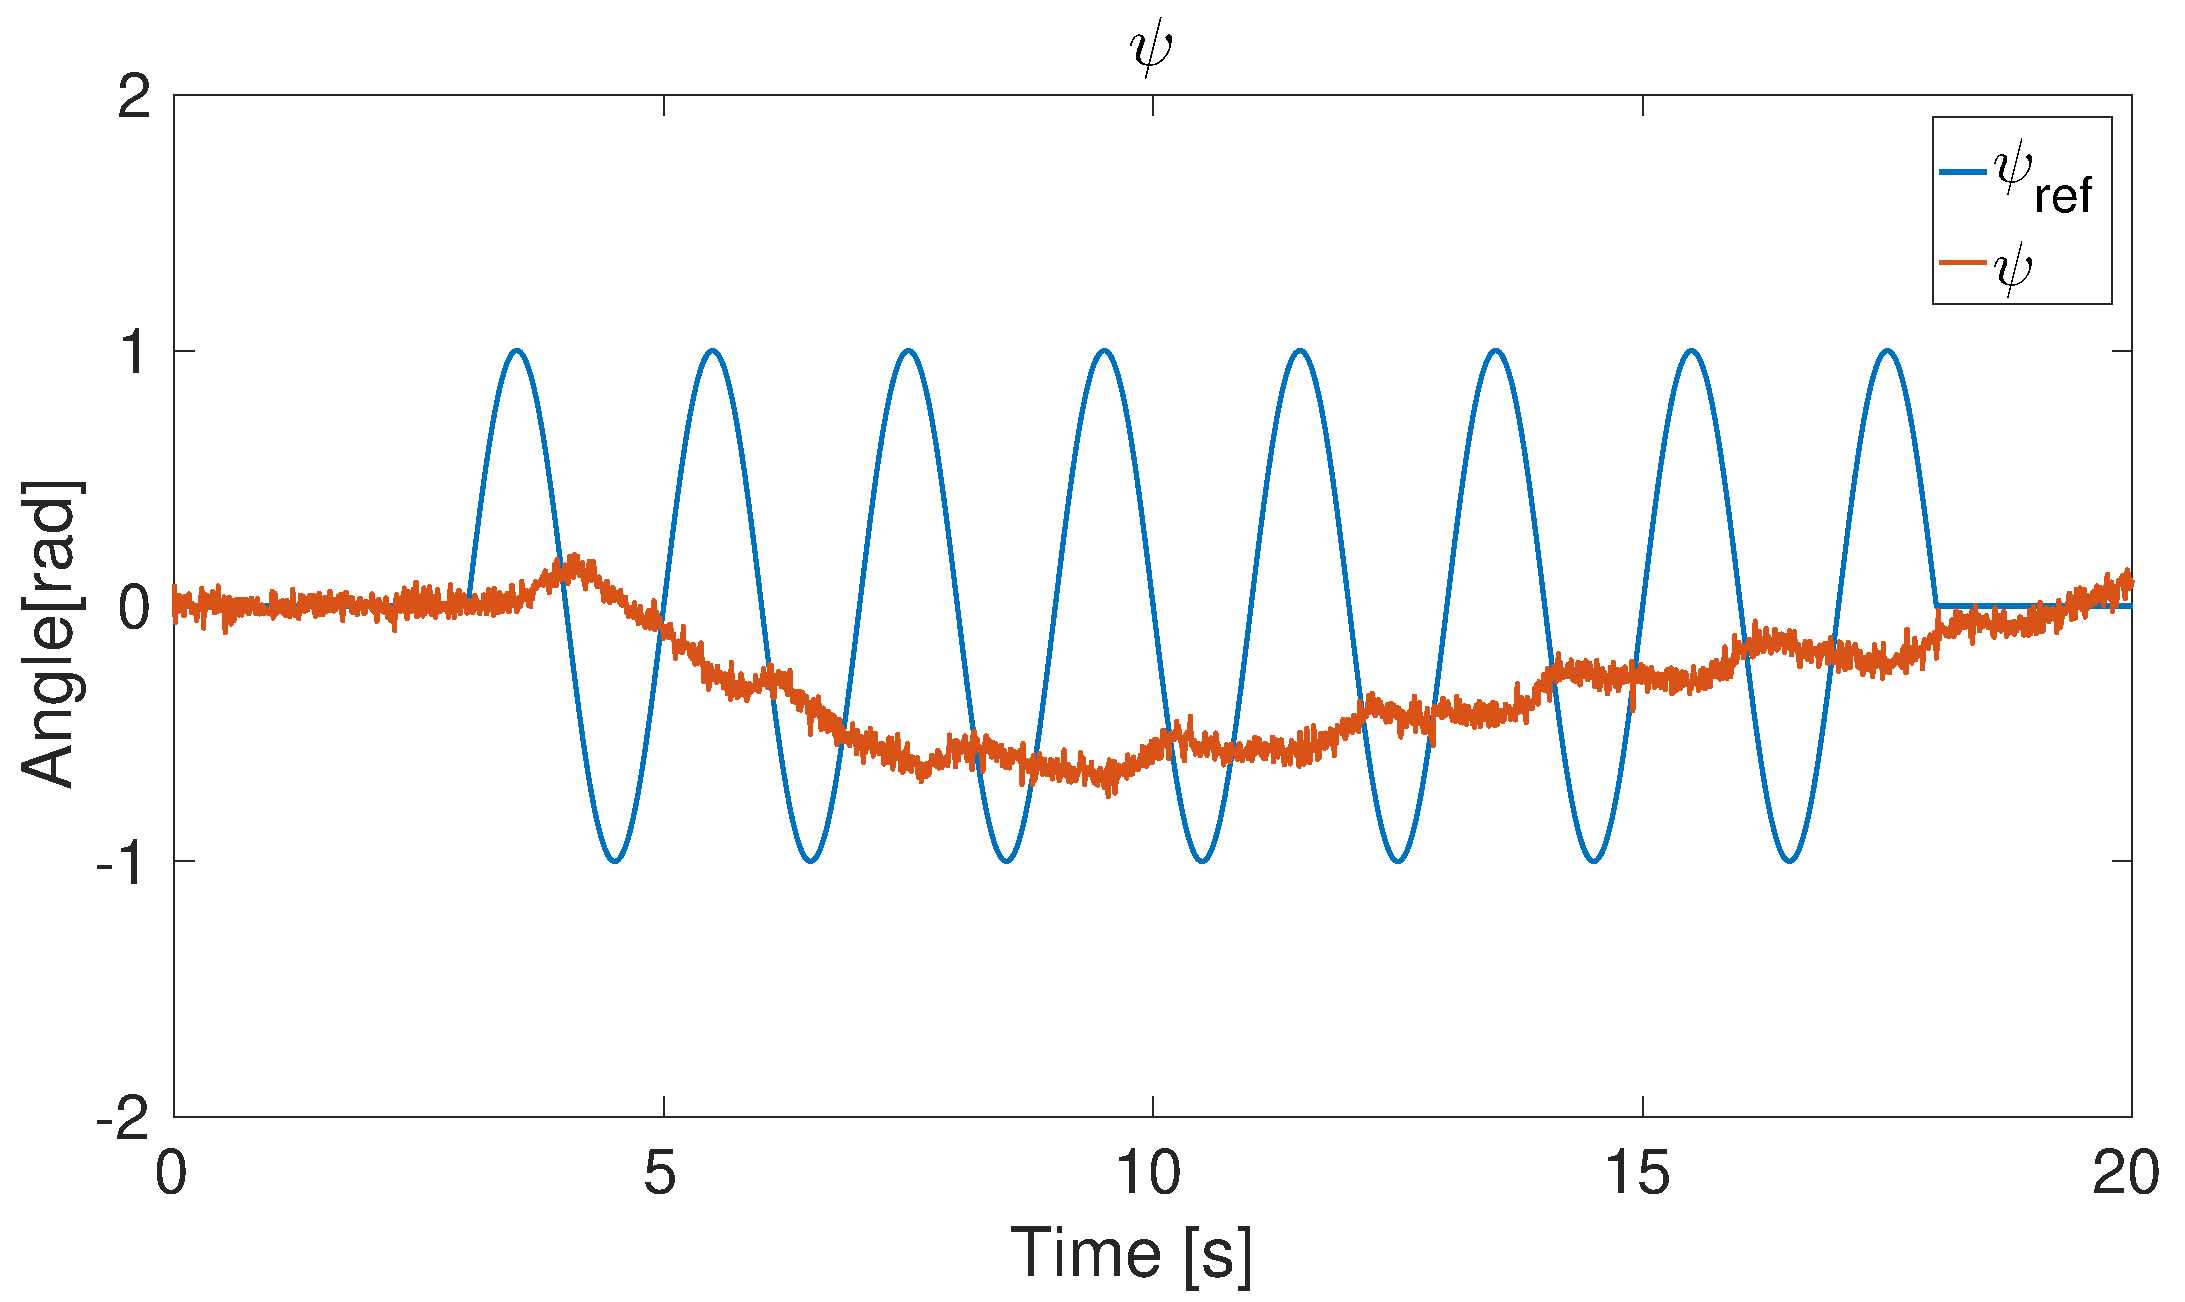
\includegraphics[width=0.4\textwidth]{simSinAllPsiA1}}
  \caption{\label{fig:SinAllAttitude}%
   A sine signal with amplitude $1$ and frequency $0.5\ \hertz$ was applied in all attitude angles at the same time while using the attitude controller.}
\end{figure}

Results from an attitude test with sine reference signals of amplitude 1 and frequency $0.5\ \hertz$ can be seen in \Figureref{fig:SinAllAttitude}. The roll angle and pitch angle did not reach the desired amplitudes in the field test. However, they followed the general form of a $0.5\ \hertz$ sine with a phase shift relative to the reference signals. The same phase shift and lack of amplitude was observed in simulations. The yaw angle followed the reference signal well during the live test but had a phase shift and a bias. The simulated result in yaw angle did not follow the reference signal at all. This may be caused by the feedback being too low for the system. This is a sign of a model error. 

\begin{figure}
\centering
  \subfloat[][\label{fig:testStepPhiTheta05RollAttitude} Test response in $\rollAngle$.]{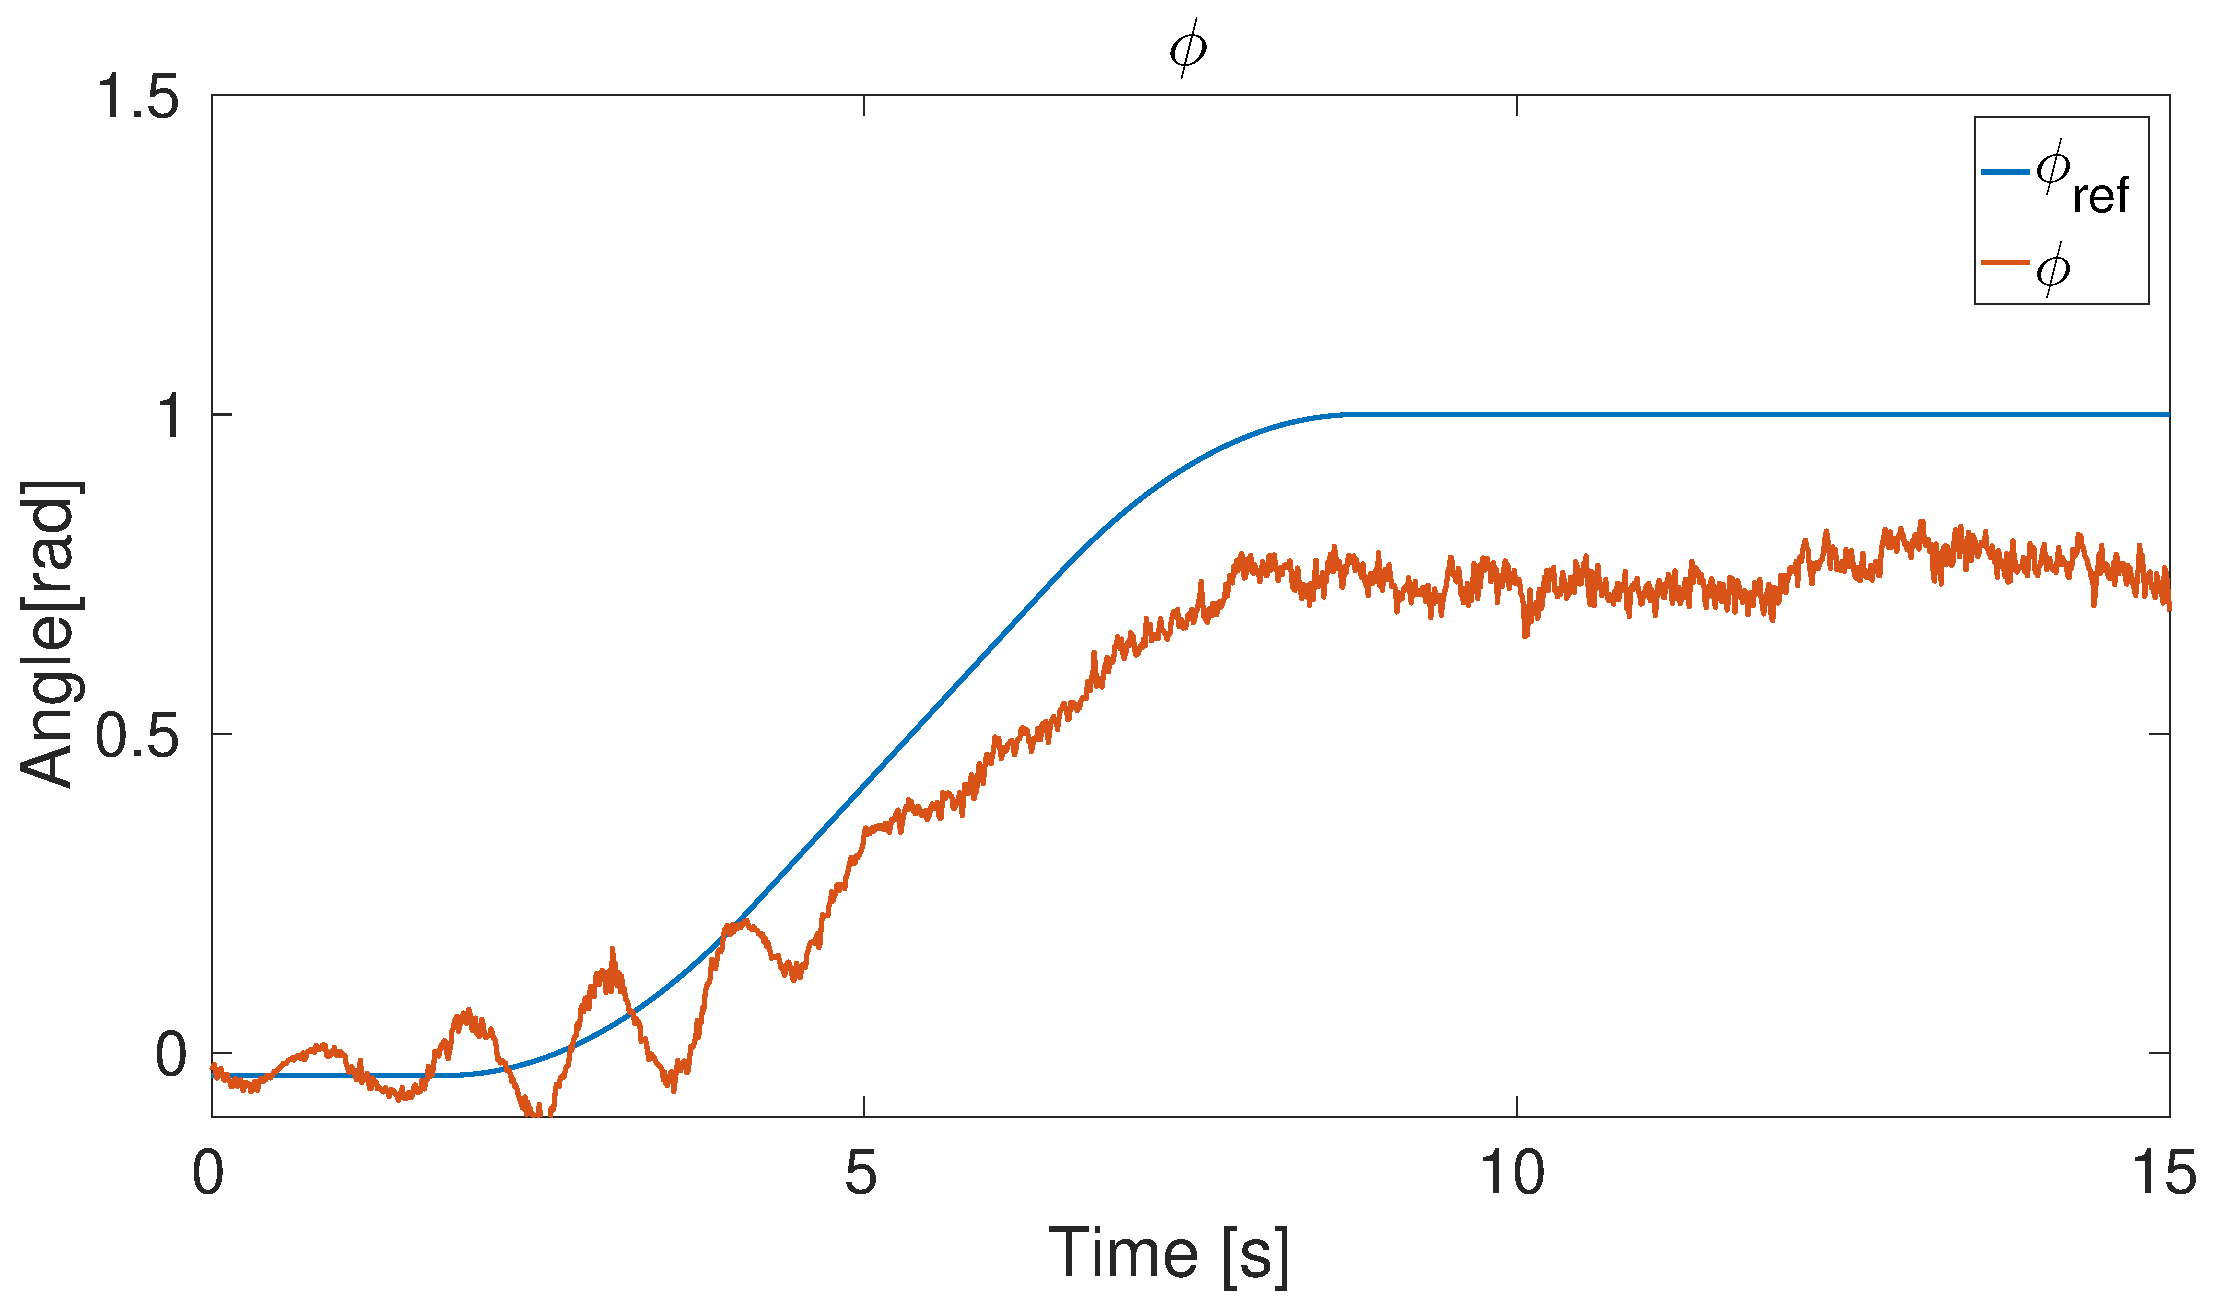
\includegraphics[width=0.4\textwidth]{testStepThetaPhiPhis3e10a1}}
  \qquad
  \subfloat[][\label{fig:simStepPhiTheta05RollAttitude} Simulated response in $\rollAngle$.]{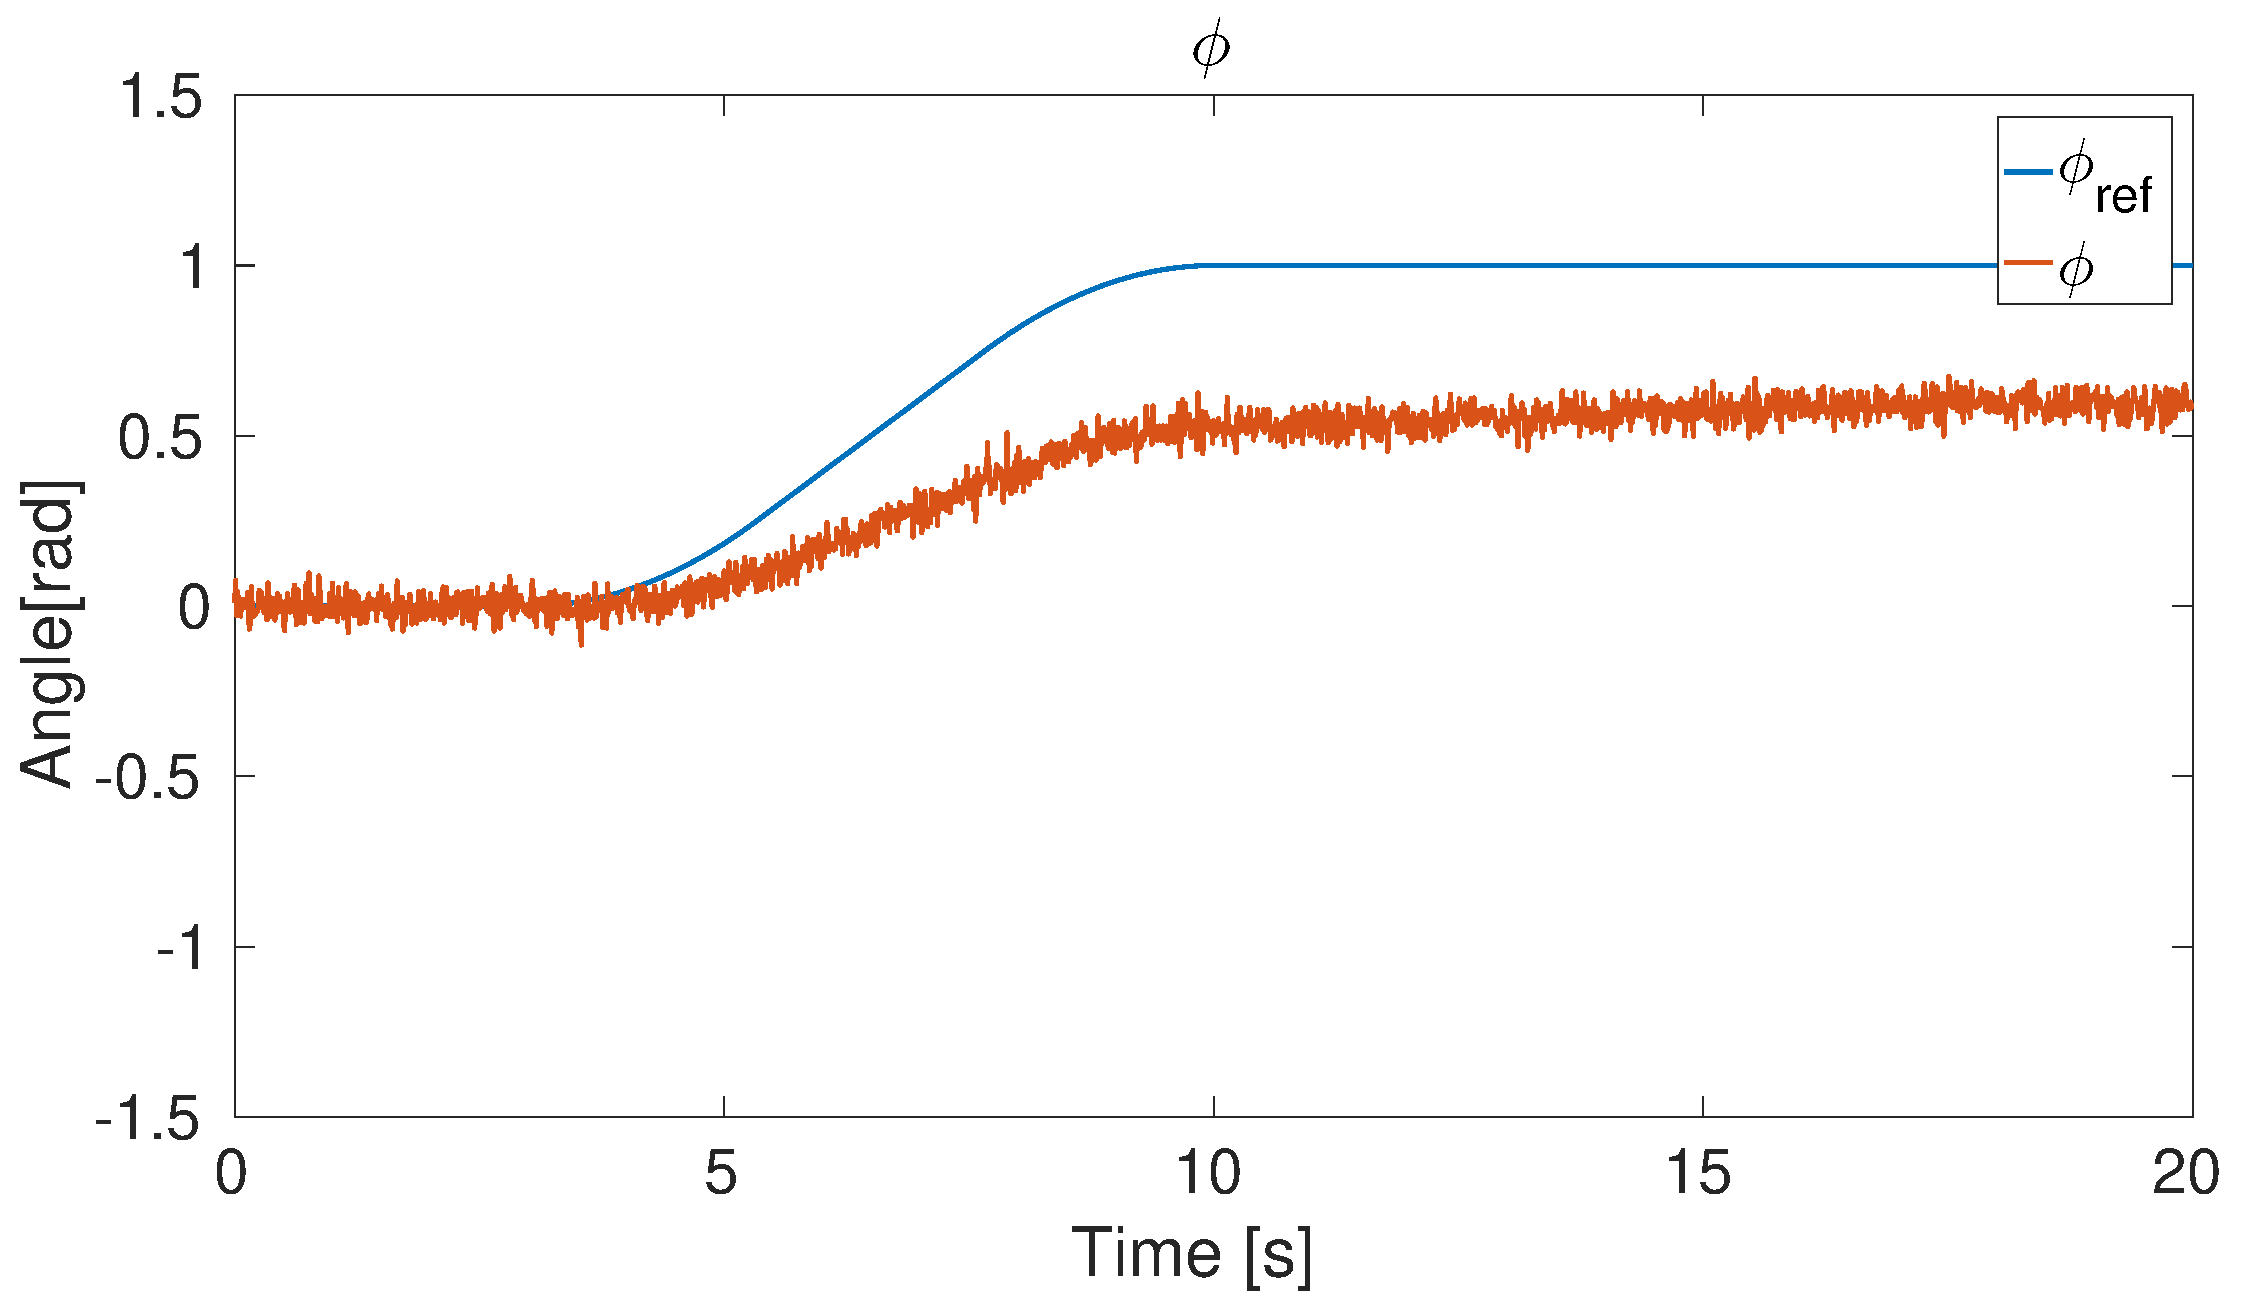
\includegraphics[width=0.4\textwidth]{simStepThetaPhiPhis3e10a1}}
  \qquad
  \subfloat[][\label{fig:testStepPhiTheta05PitchAttitude}Test response in $\pitchAngle$.]{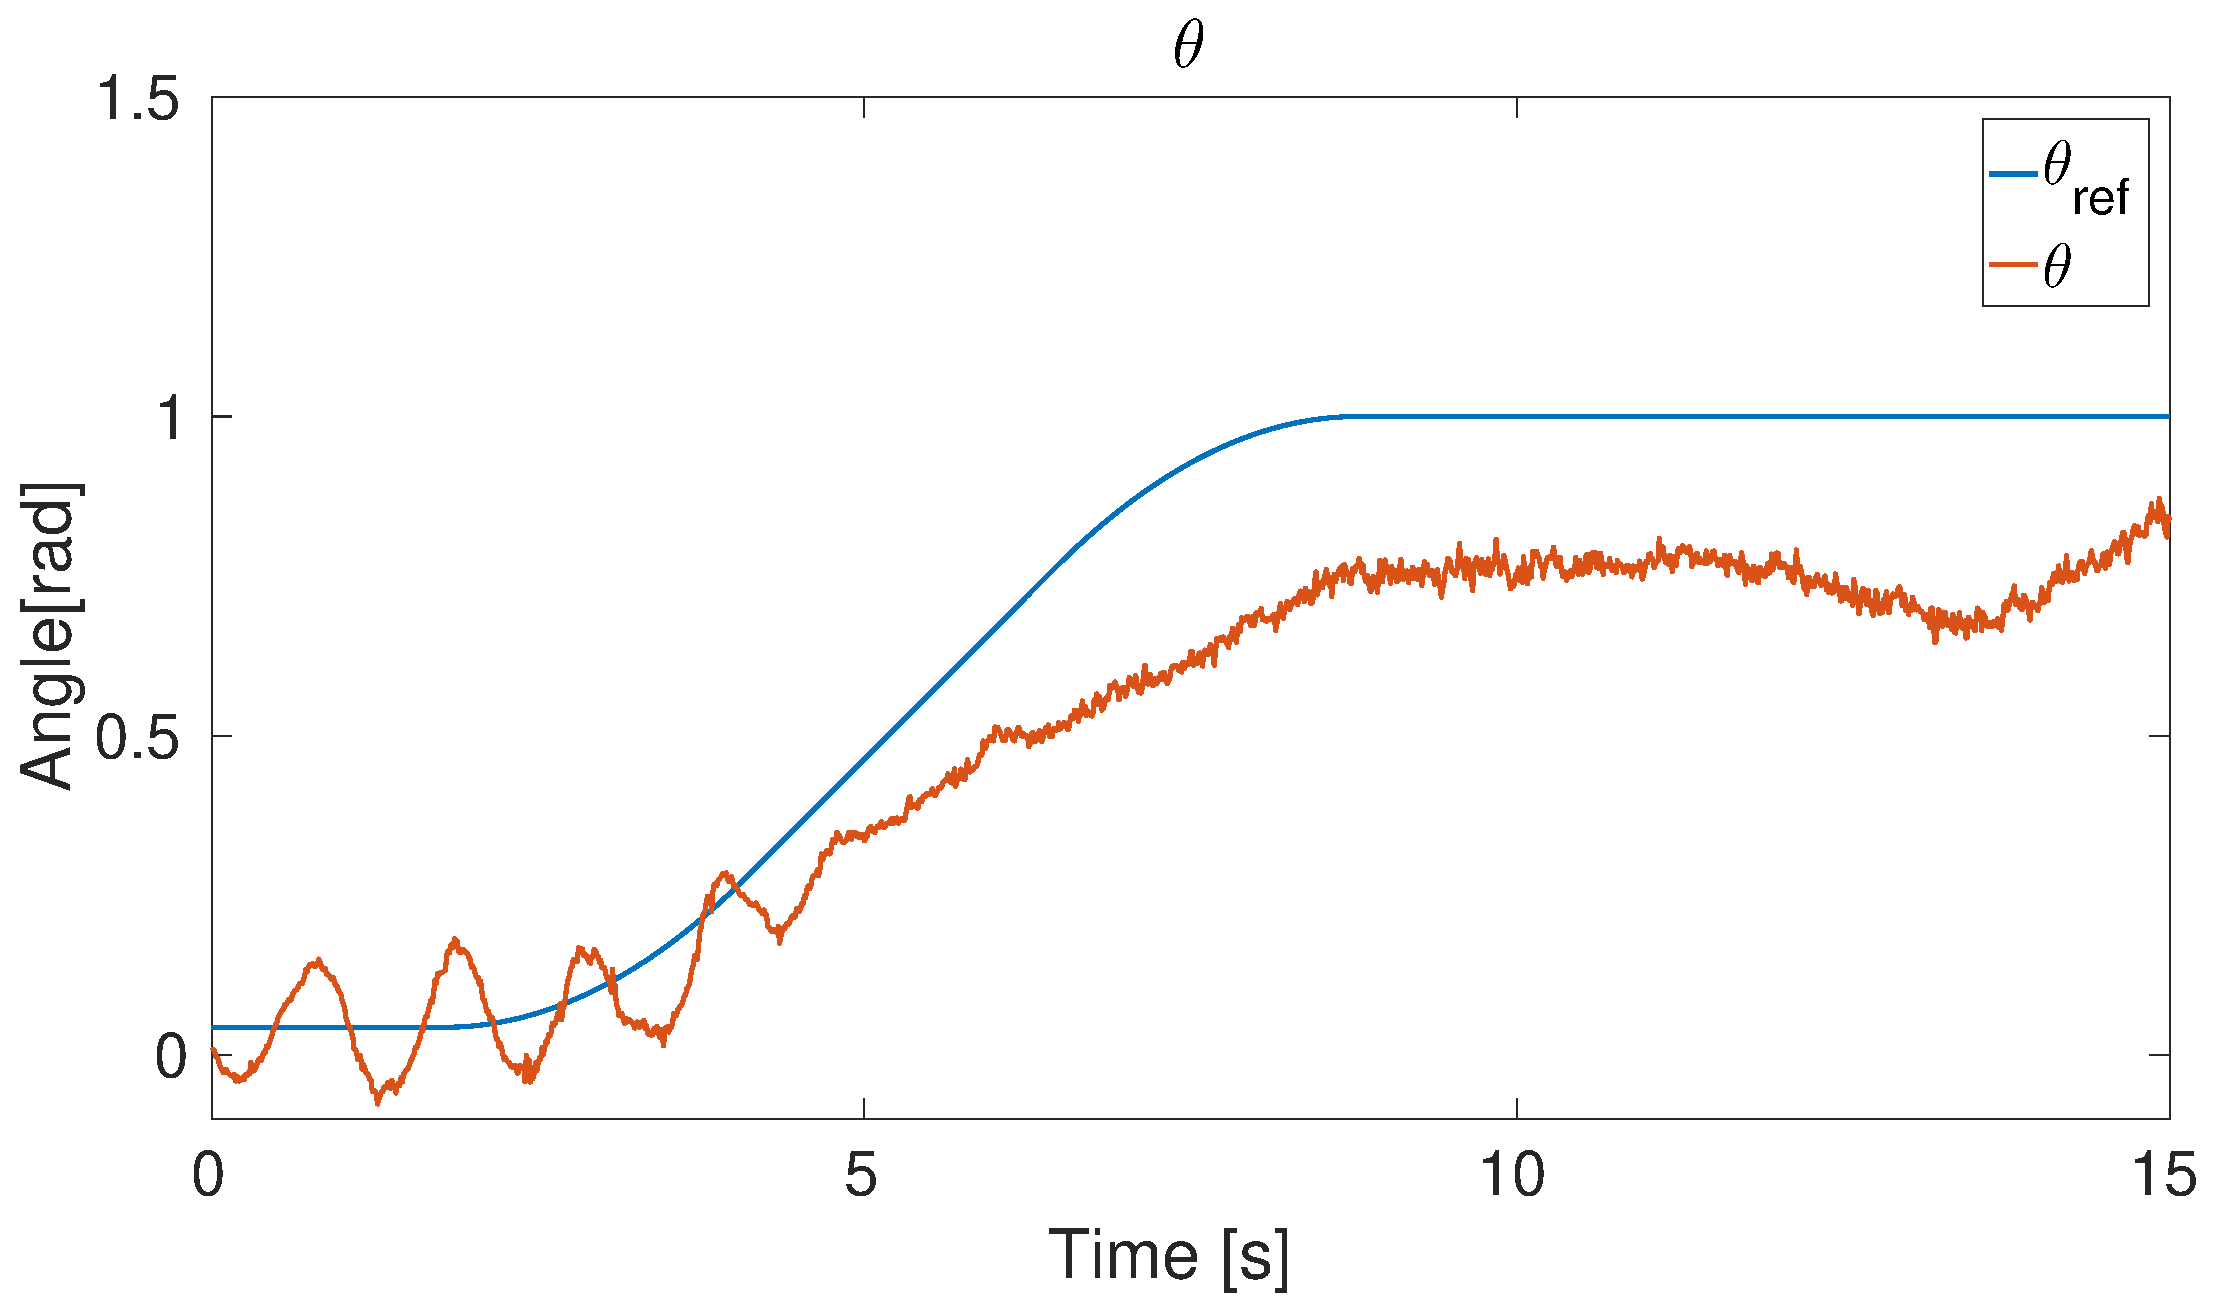
\includegraphics[width=0.4\textwidth]{testStepThetaPhiThetas3e10a1}}
  \qquad
  \subfloat[][\label{fig:simStepPhiTheta05PitchAttitude} Simulated response in $\pitchAngle$.]{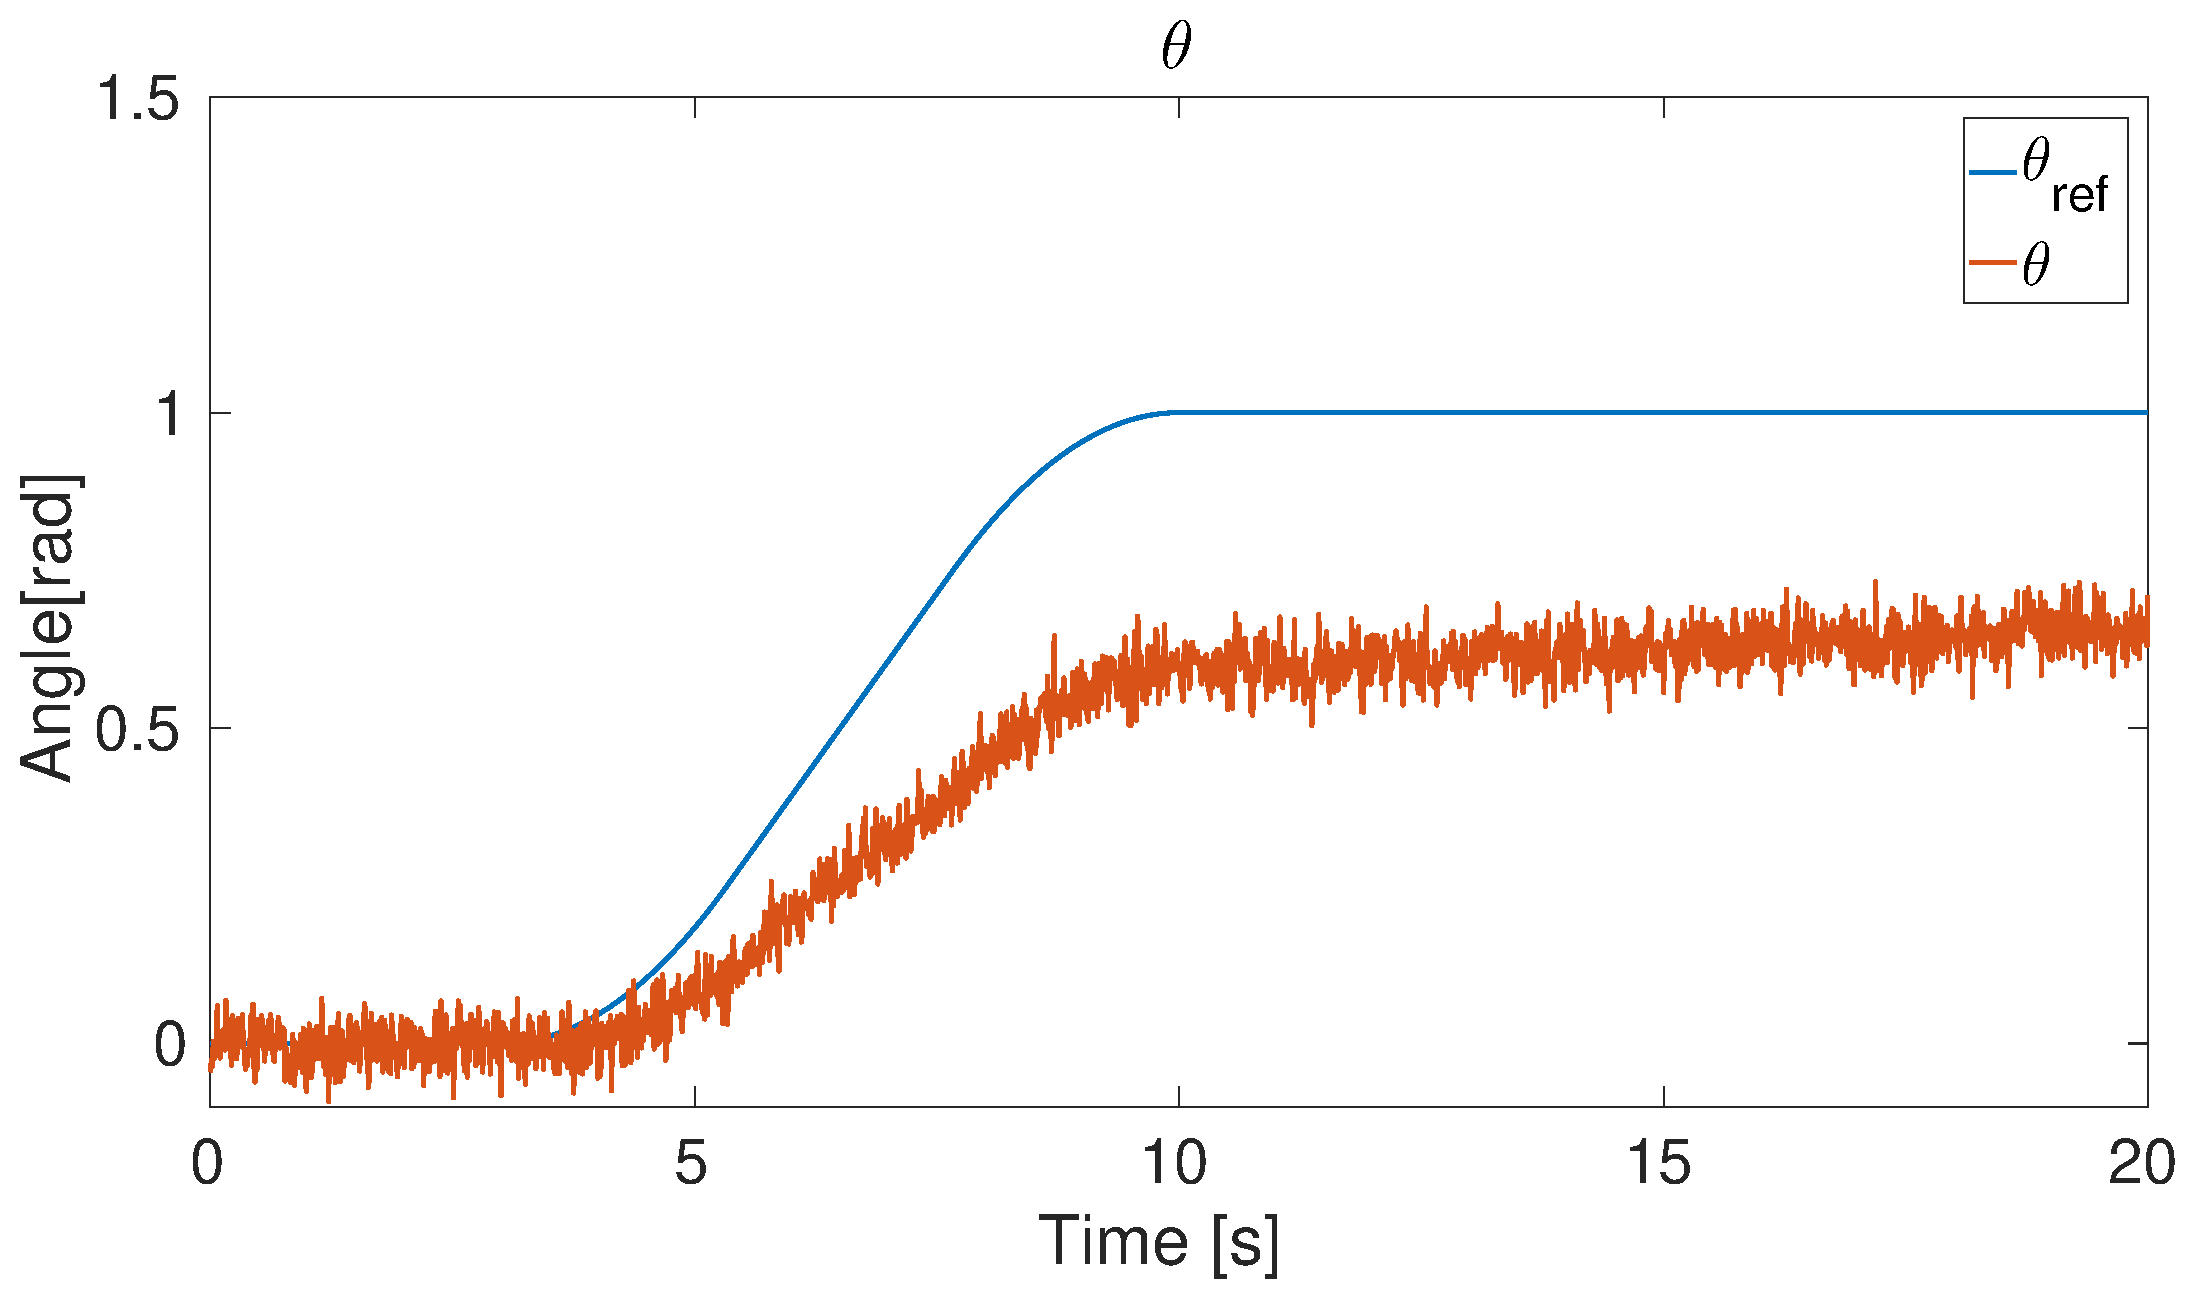
\includegraphics[width=0.4\textwidth]{simStepThetaPhiThetas3e10a1}}
  \caption{\label{fig:StepPhiThetaAttitude}%
  Smooth steps with $q_{\text{0}} = 0$, $q_{\text{f}} = 1$, $t_{\text{s}} = 3$, $t_{\text{f}} = 15$ and $V = 1.5 (q_{\text{f}} - q_{\text{0}})/(t_{\text{f}} - t_{\text{s}}))$ were applied in \pitchAngle and \rollAngle at the same time while using the attitude controller. The attitude angle $\yawAngle$ was kept free during the test.}
\end{figure}

The result from a smooth step test in roll angle and pitch angle can be seen in \Figureref{fig:StepPhiThetaAttitude}. During the test, the yaw angle was kept free. Both the roll angle and the pitch angle followed the shape of the reference signal but did not reach the desired magnitude. The steady-state errors for roll and pitch angle were approximately $0.35$. The simulated result in roll angle and pitch angle performed worse than the live test. The simulated roll angle had a steady-state error $0.5$ and the steady-state error in pitch angle was $0.4$.

%%%%%%%%%%%%%%%%%%%%%%%%%%%Rate%%%%%%%%%%%%%%%%
\begin{figure}
\centering
  \subfloat[][\label{fig:testStepAllPRate} Test response in $\rollVelocity$.]{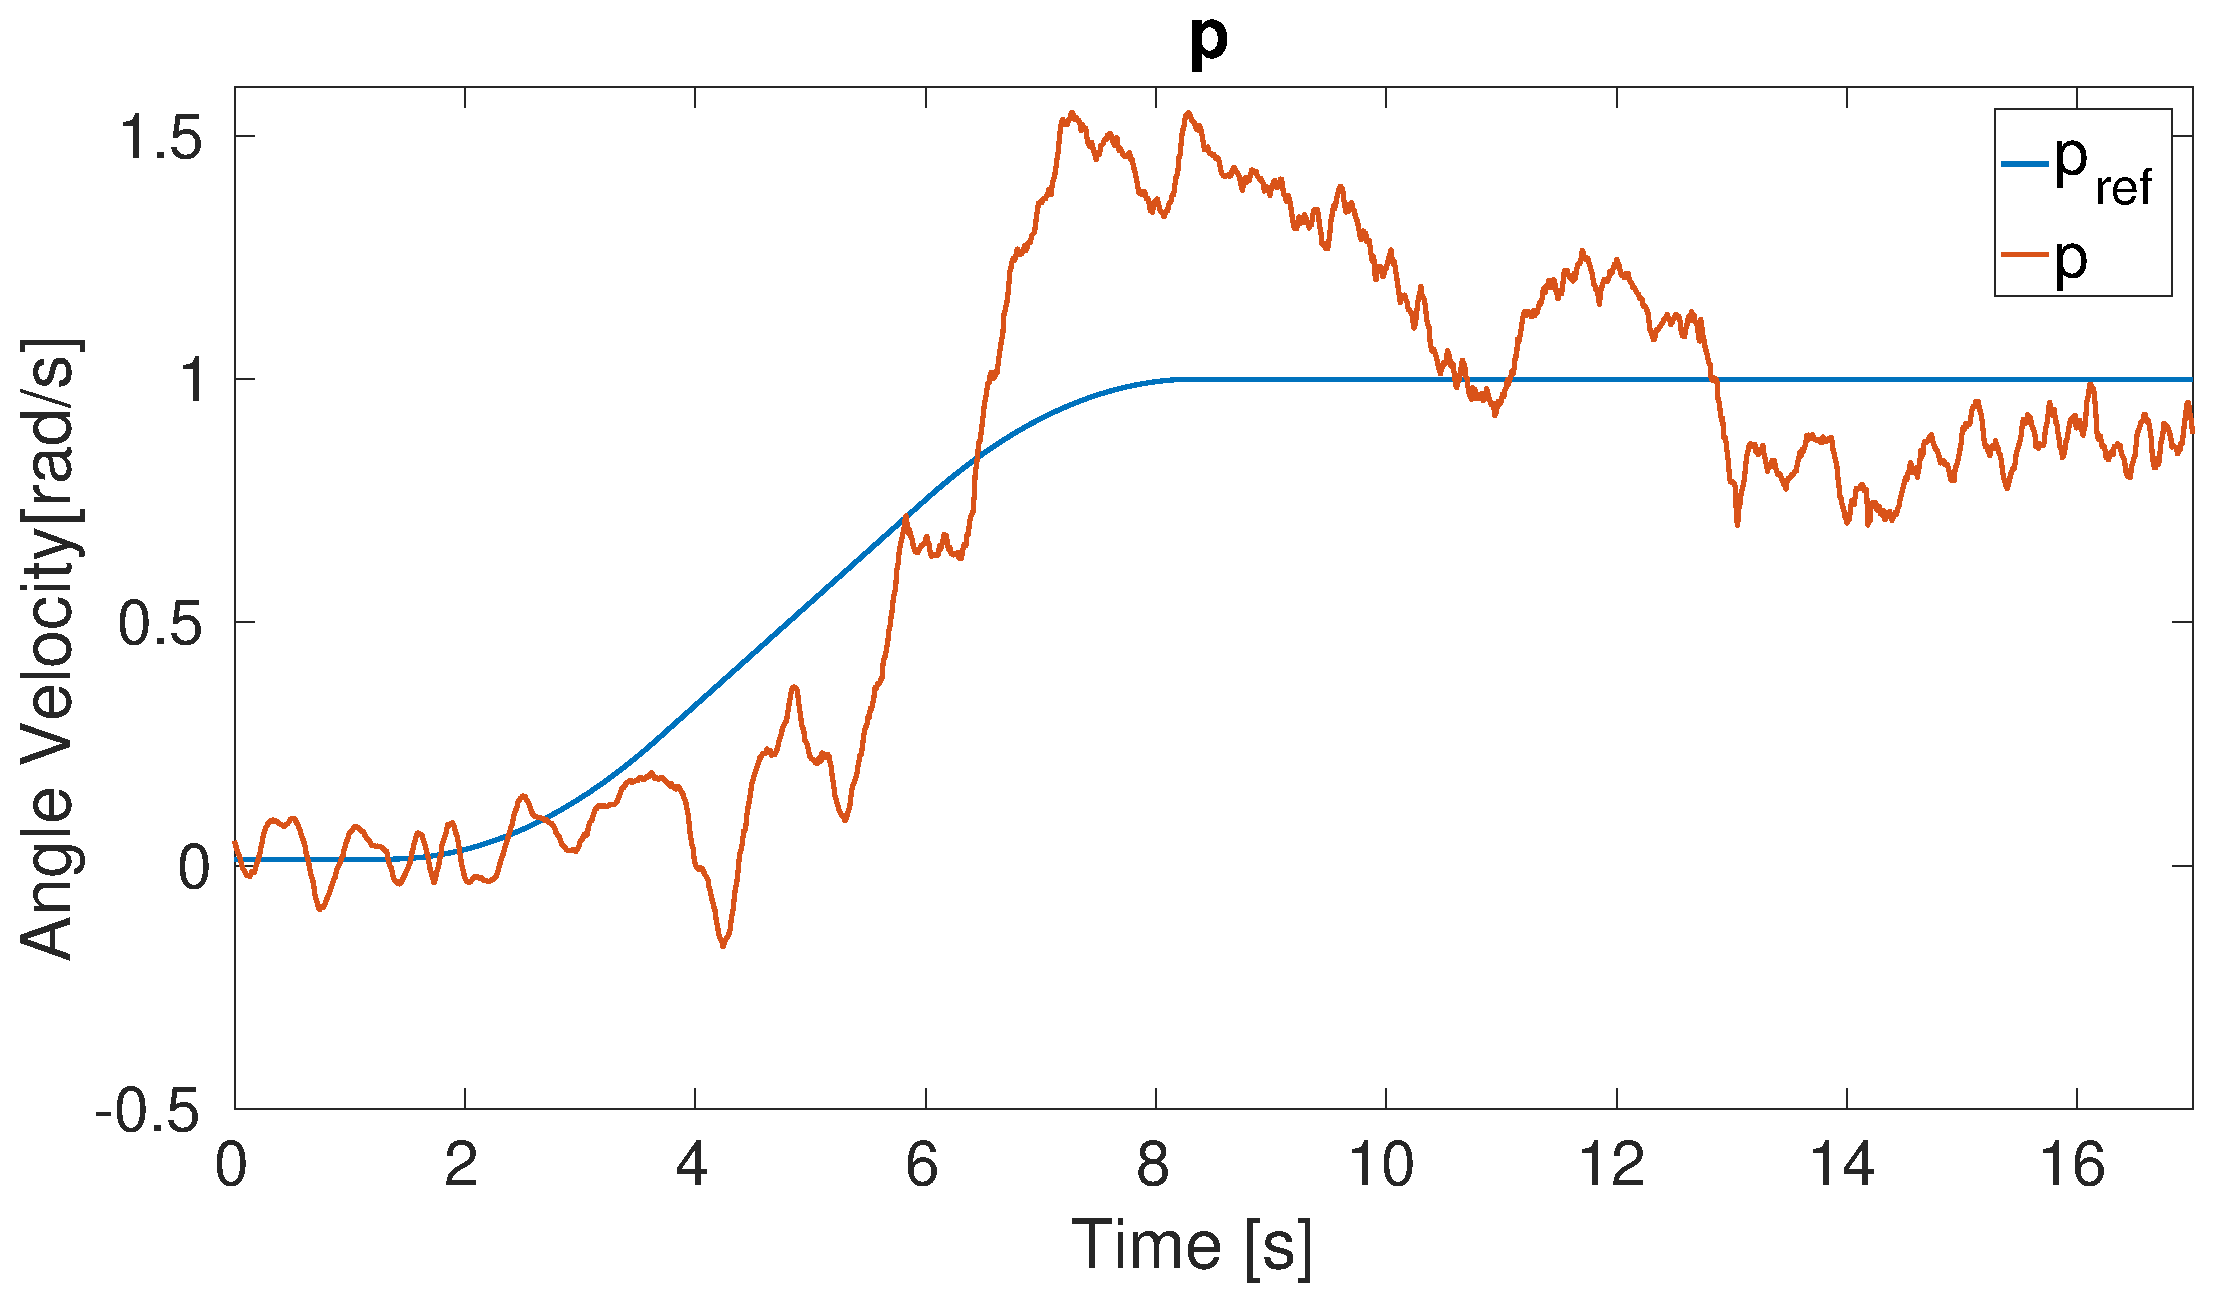
\includegraphics[width=0.4\textwidth]{testStepAllPs3e10a1}}
  \qquad 
  \subfloat[][\label{fig:simStepAllPRate} Simulated response in $\rollVelocity$.]{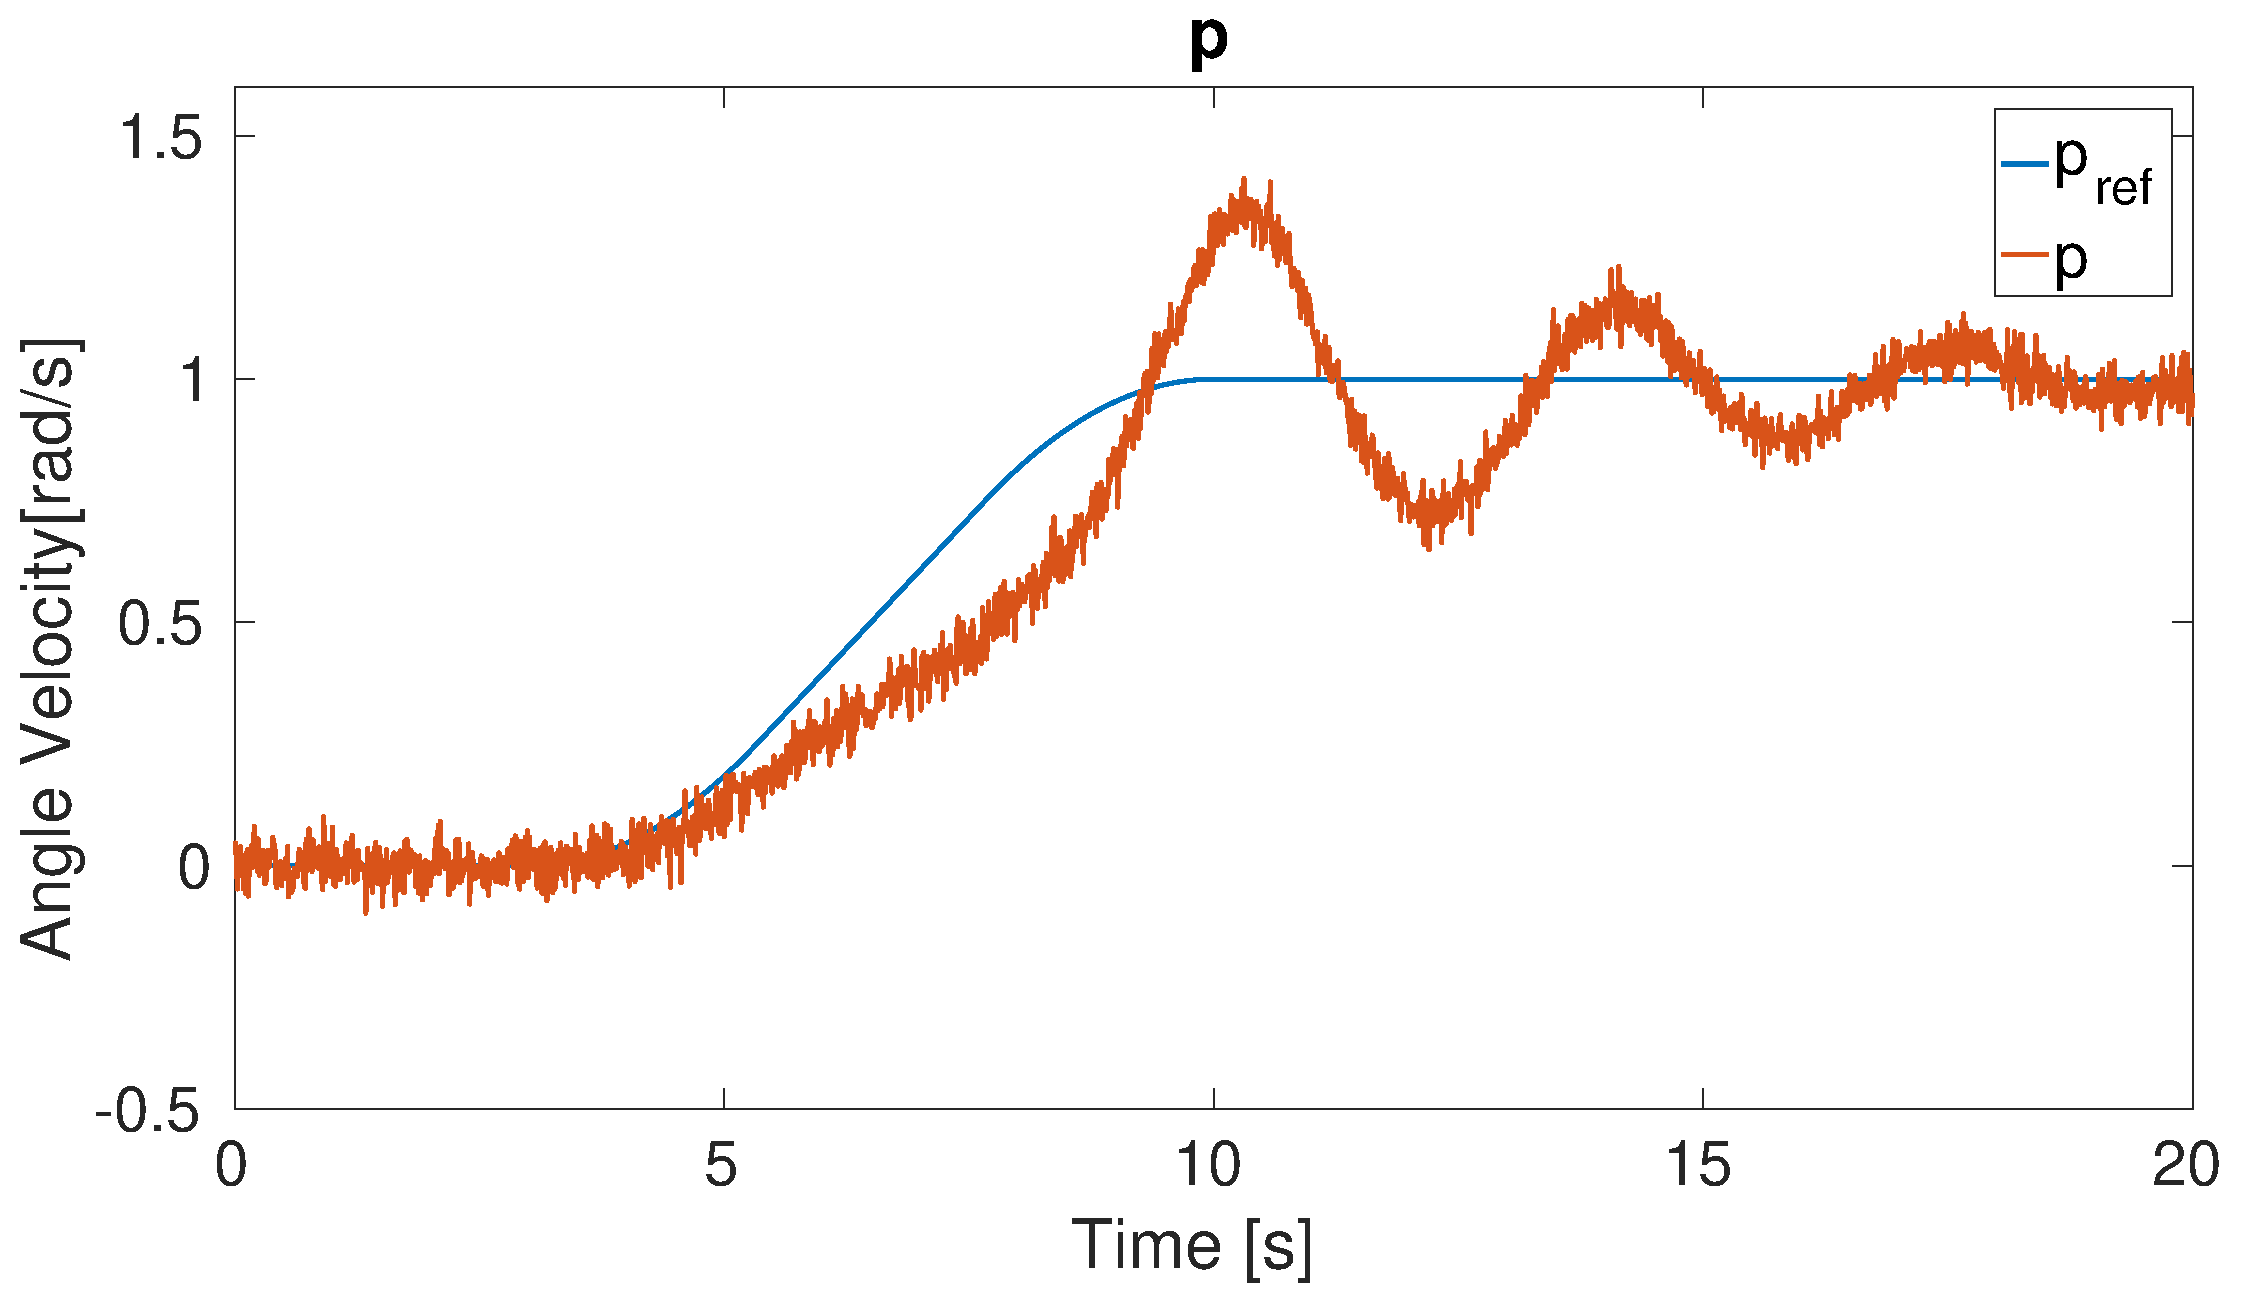
\includegraphics[width=0.4\textwidth]{simStepAllPs3e10a1}}
  \qquad
  \subfloat[][\label{fig:testStepAllQRate} Test response in $\pitchVelocity$.]{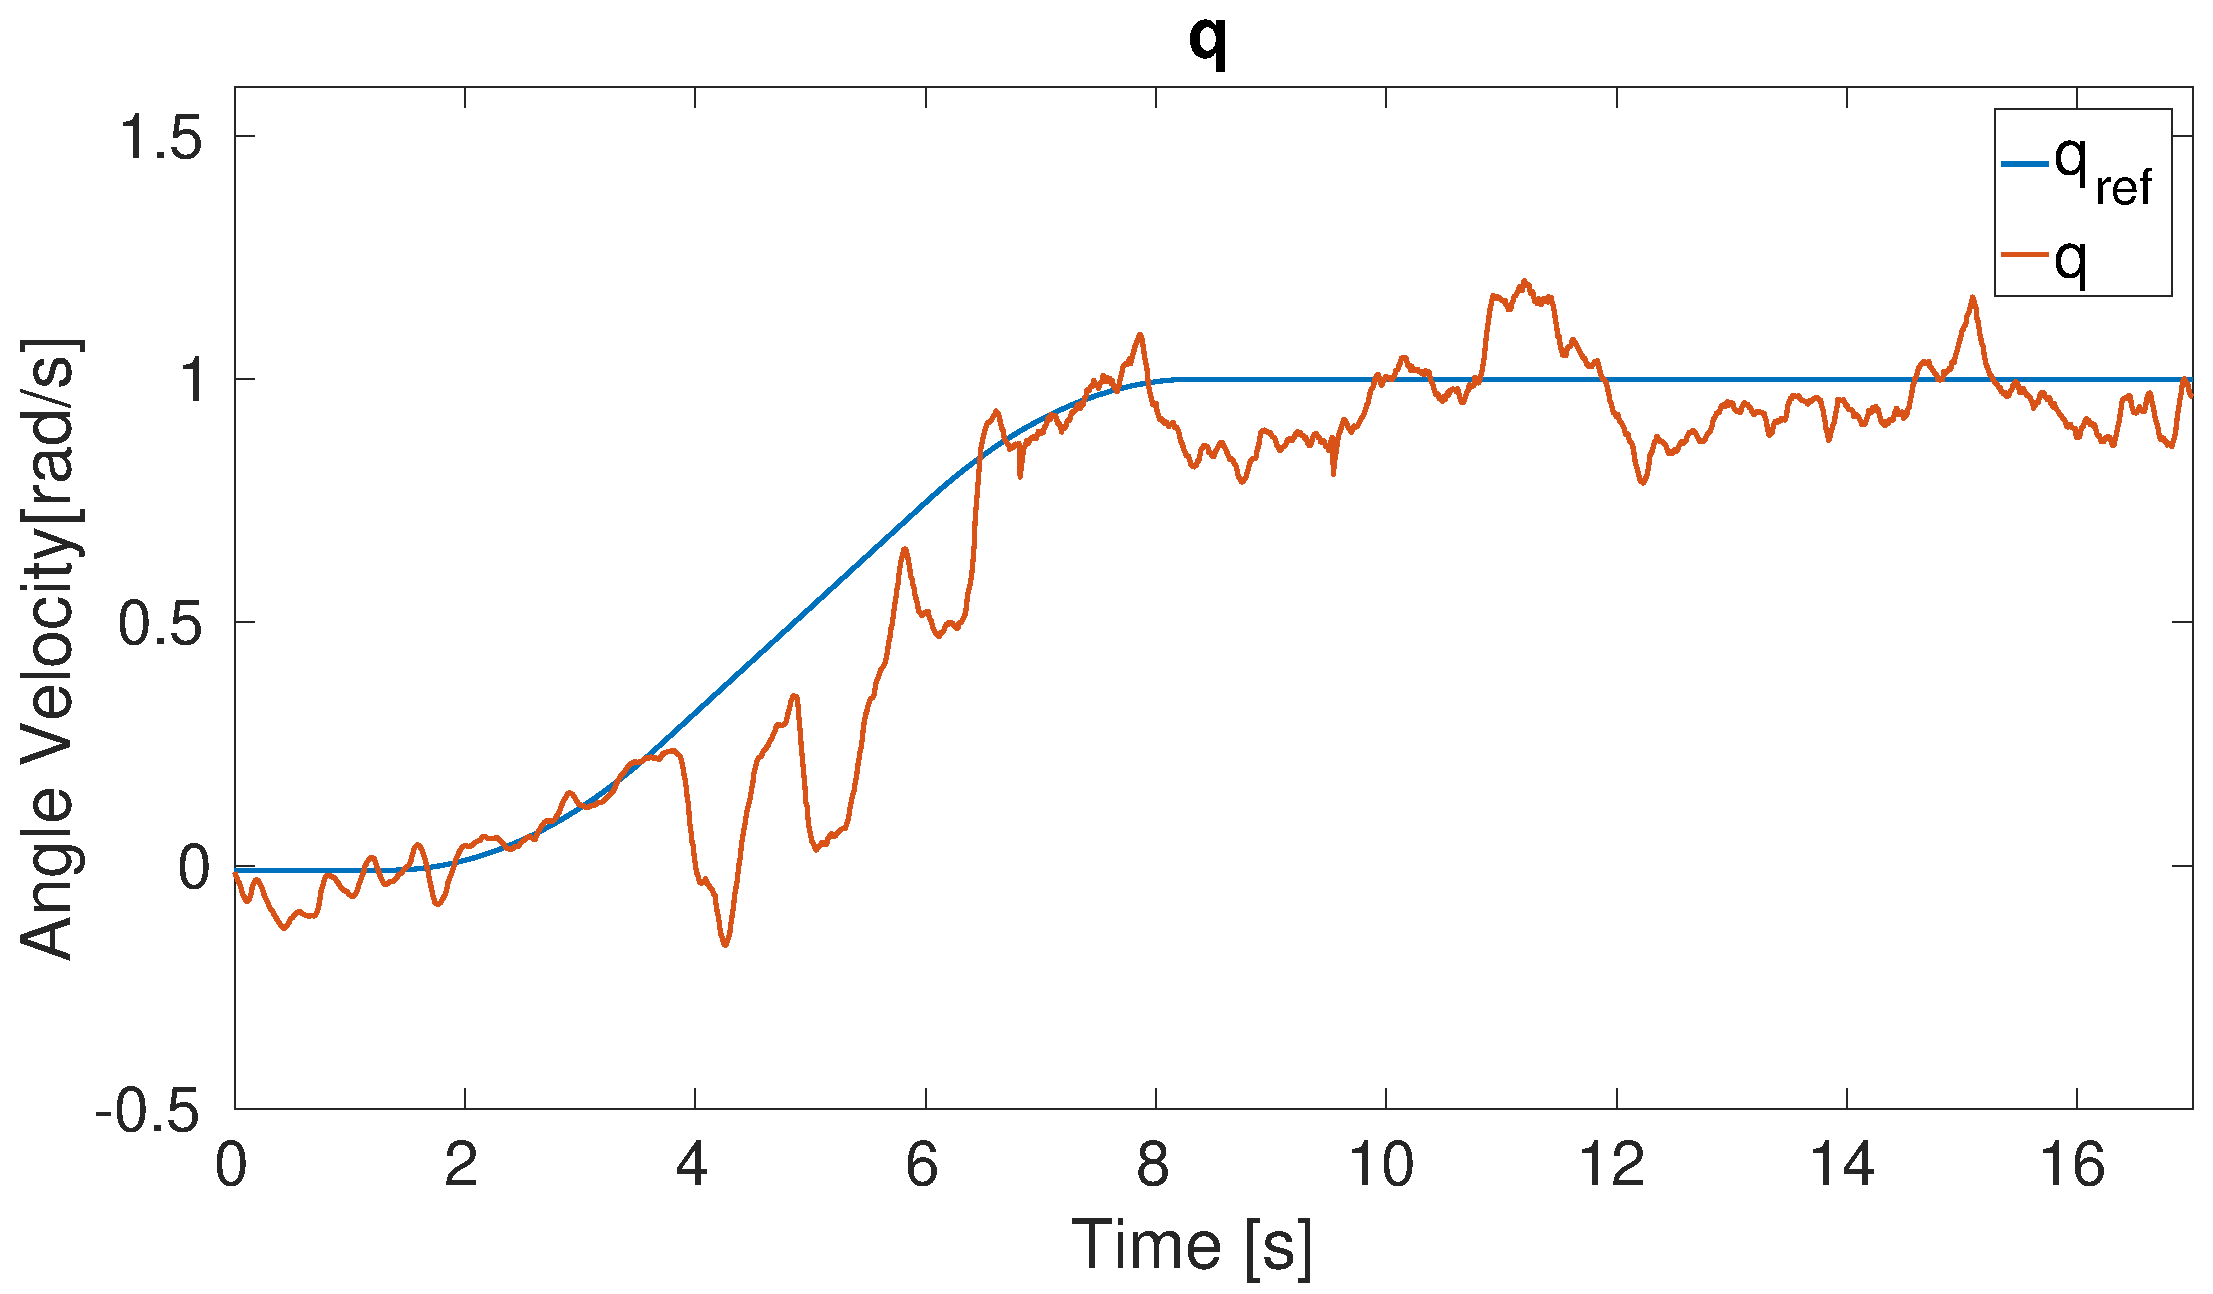
\includegraphics[width=0.4\textwidth]{testStepAllQs3e10a1}}
  \qquad
  \subfloat[][\label{fig:simStepAllQRate} Simulated response in $\pitchVelocity$.]{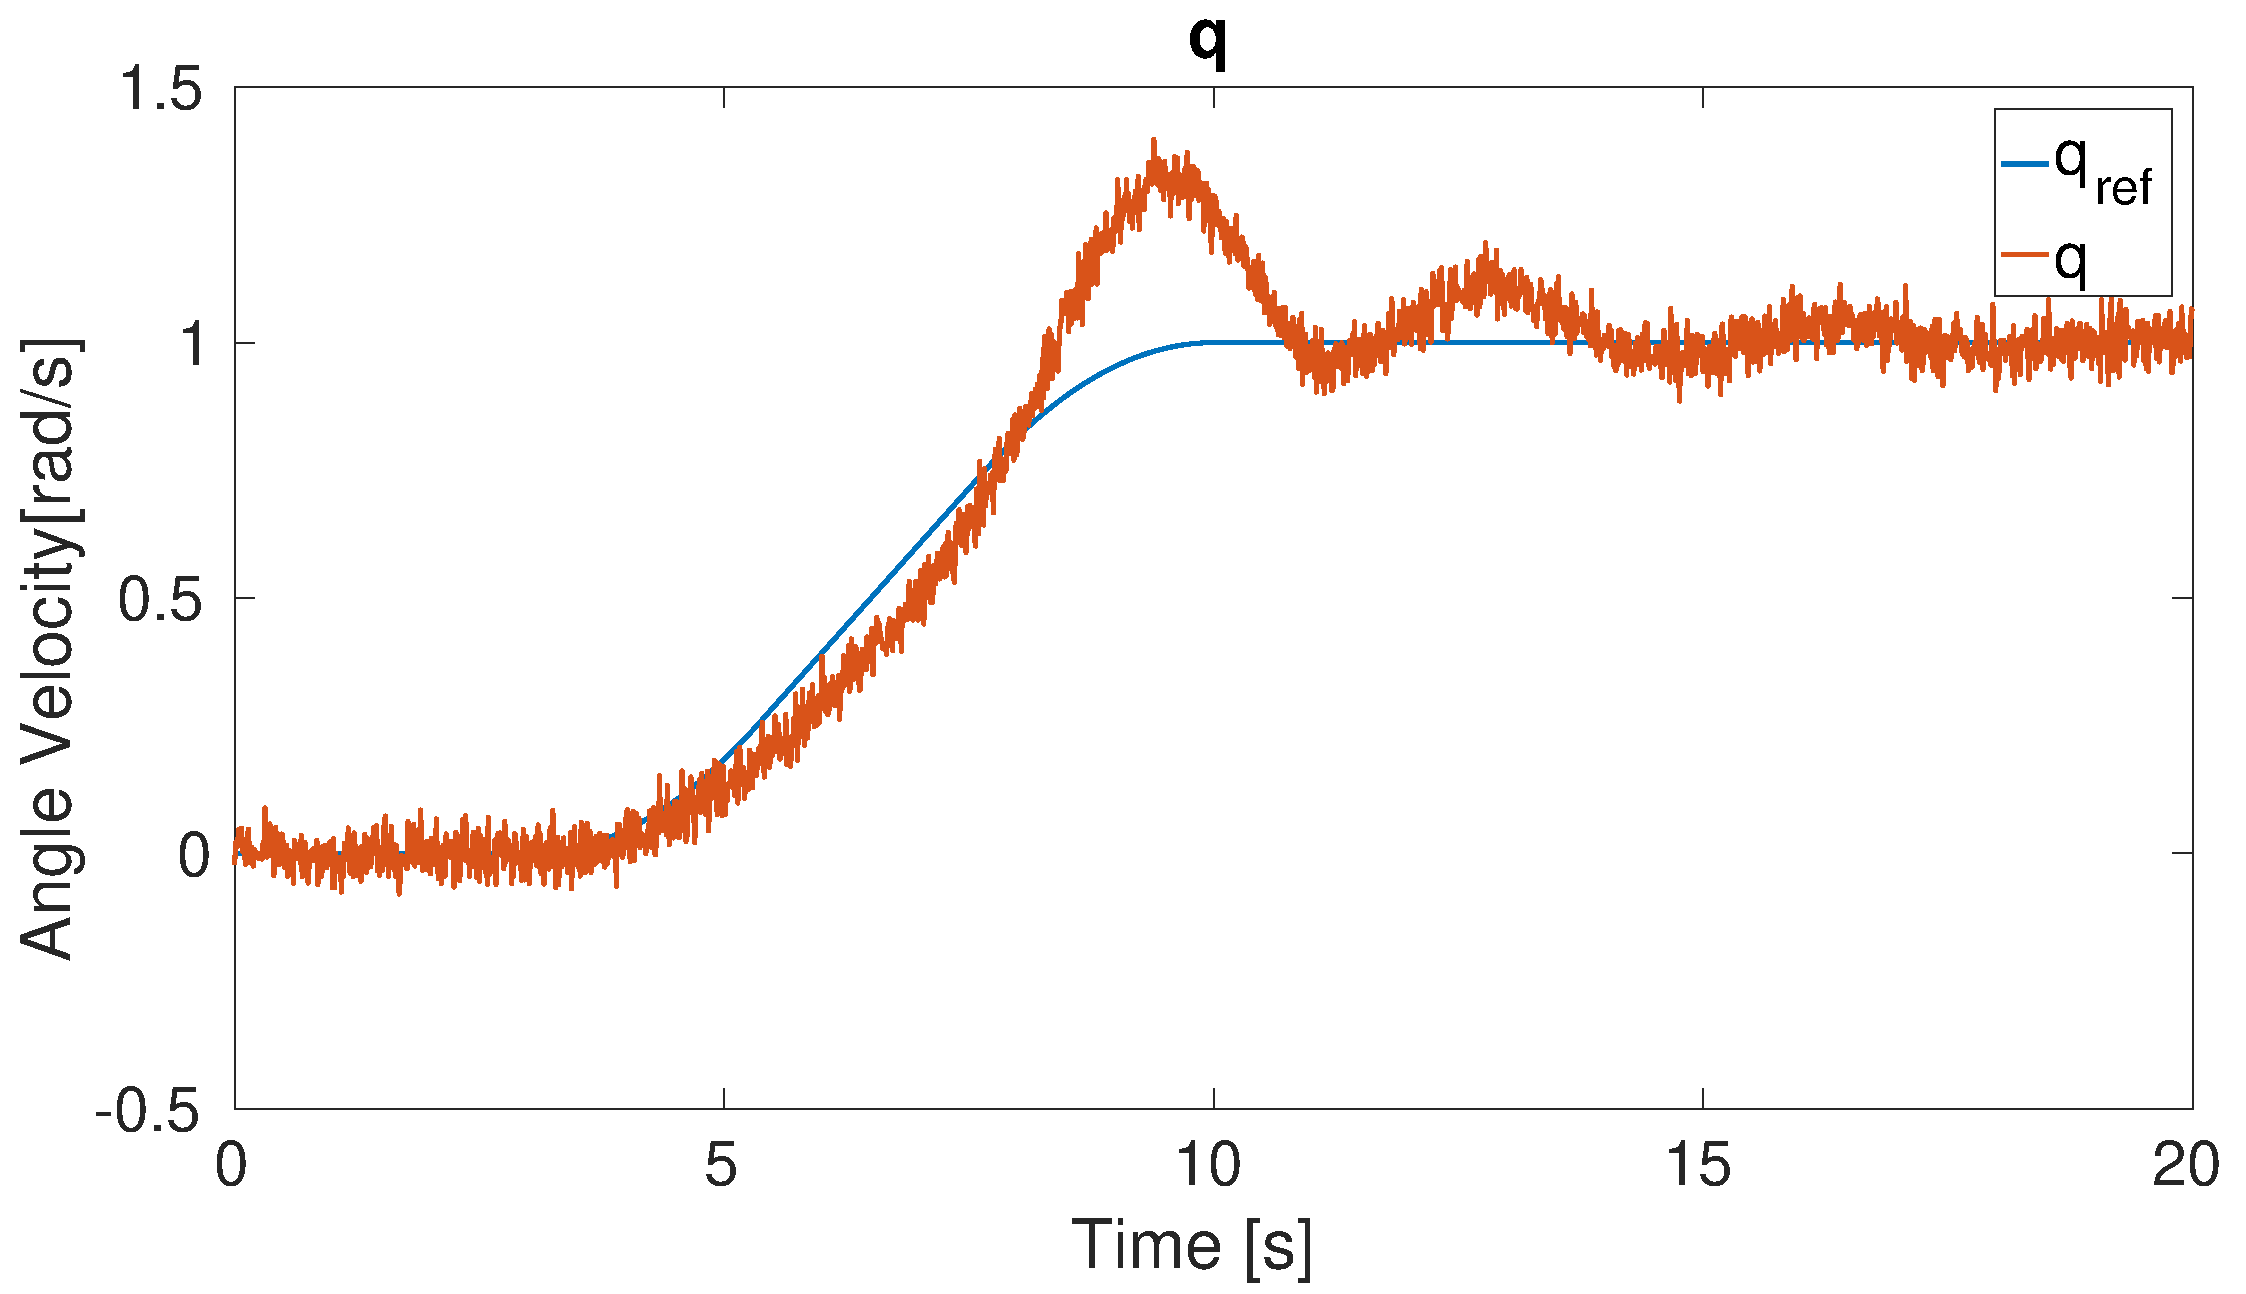
\includegraphics[width=0.4\textwidth]{simStepAllQs3e10a1}}
  \qquad
  \subfloat[][\label{fig:testStepAllRRate} Test response in $\yawVelocity$.]{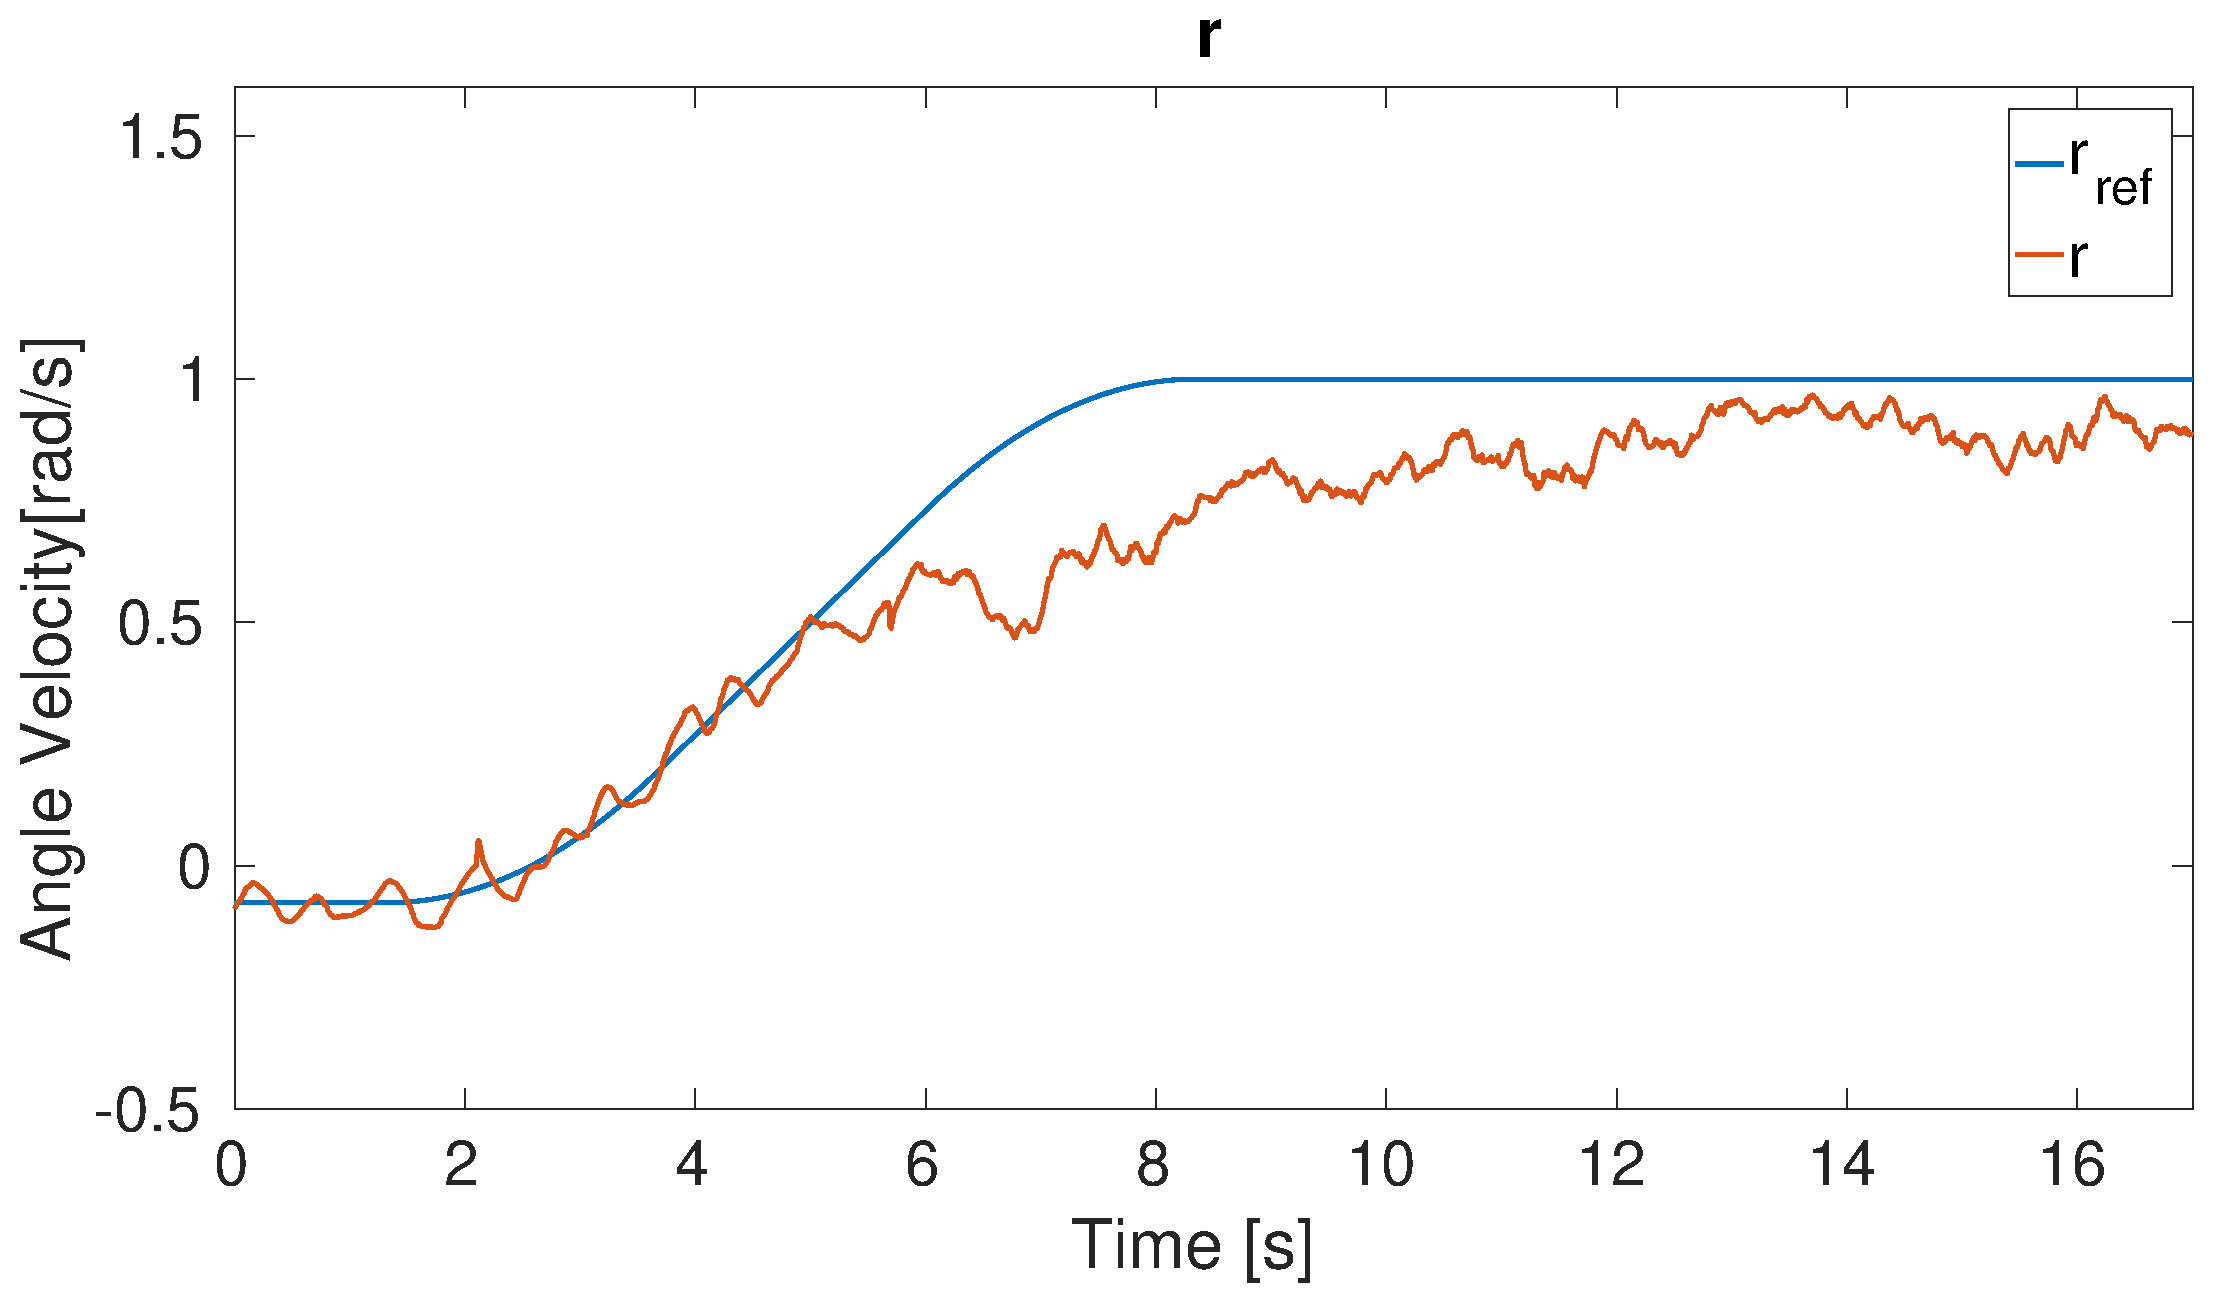
\includegraphics[width=0.4\textwidth]{testStepAllRs3e10a1}}
  \qquad
  \subfloat[][\label{fig:simStepAllRRate} Simulated response in $\yawVelocity$.]{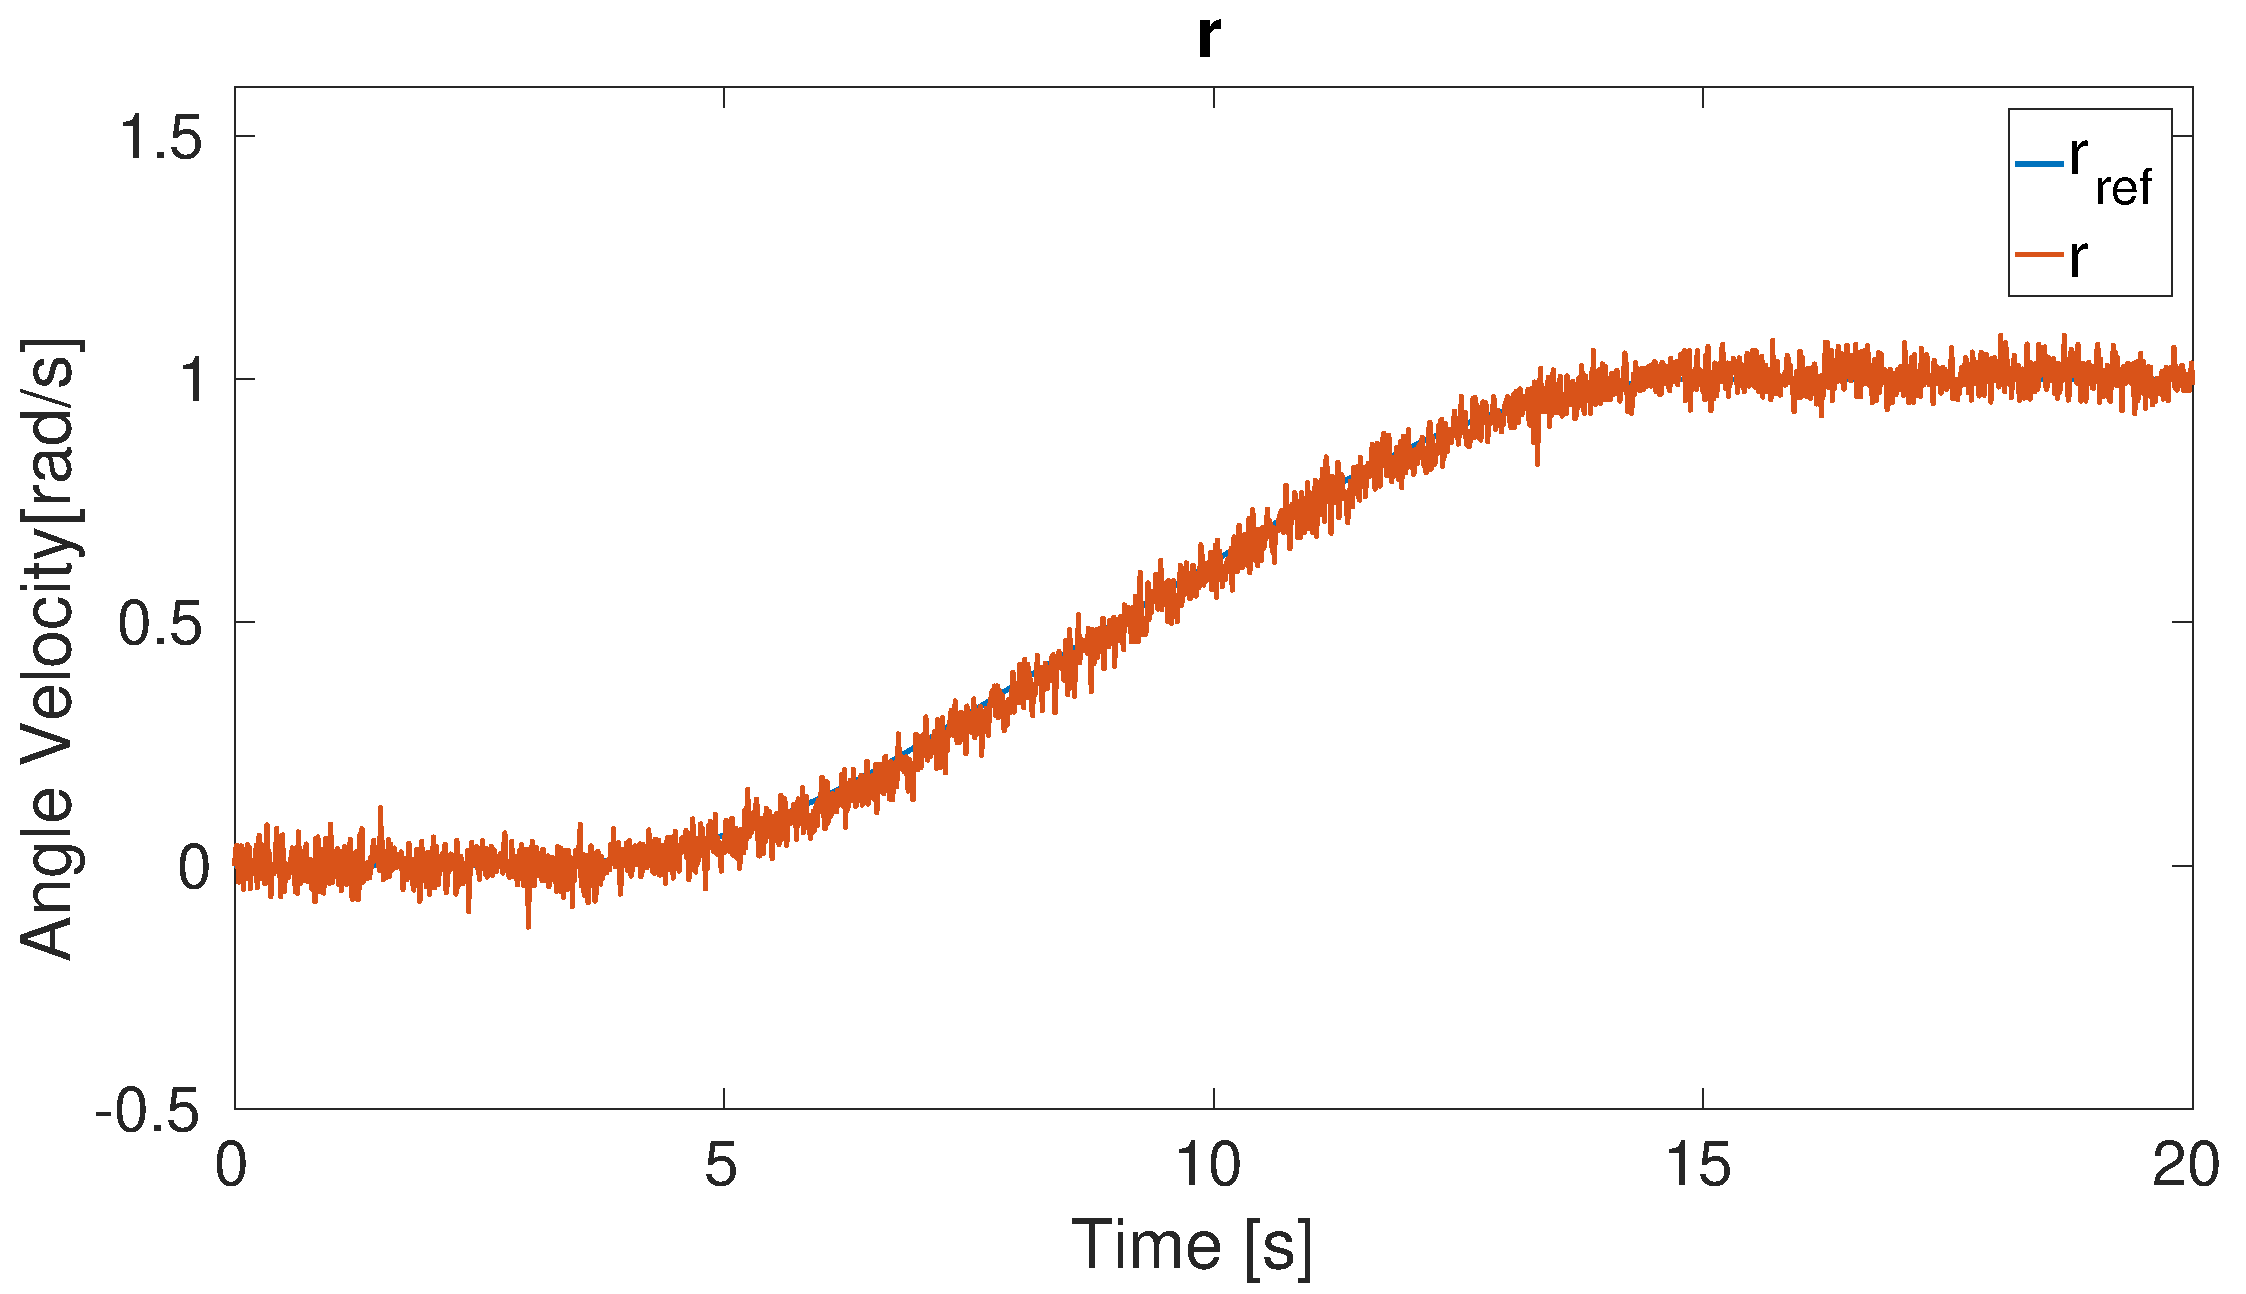
\includegraphics[width=0.4\textwidth]{simStepAllRs3e10a1}}
  \caption{\label{fig:StepAllRate}% 
  A smooth step with $q_{\text{0}} = 0$, $q_{\text{f}} = 1$, $t_{\text{s}} = 3$, $t_{\text{f}} = 15$ and $V = 1.5 (q_{\text{f}} - q_{\text{0}})/(t_{\text{f}} - t_{\text{s}}))$ was applied in all angular velocities at the same time while using the angular velocity controller.}
\end{figure}

\Figureref{fig:StepAllRate} shows a smooth step applied in all angular velocities while using the angular velocity controller. An overshoot of $0.5$ was obtained in $\rollVelocity$ for the field test while the simulation it only had an overshoot of $0.2$ but suffers from stronger oscillations. Both the field test and the simulation in $\rollVelocity$ followed the reference signal and had a small steady-state error. 

The field and simulated test in $\pitchVelocity$ followed the reference value well and had negligible steady-state errors with some oscillative behaviour. Moreover, the field test had no overshoot while the simulation in $\pitchVelocity$ had stronger oscillations and an overshoot of $0.4$. 

The simulated test in $\yawVelocity$ performed well and followed the reference relatively well. The field test in $\yawVelocity$ performed well, but it was slow to rise to the requested reference signal and had a small steady-state error of $0.1$. 

\begin{figure}
\centering
  \subfloat[][\label{fig:testSinAllPRate} Test response in $\rollVelocity$.]{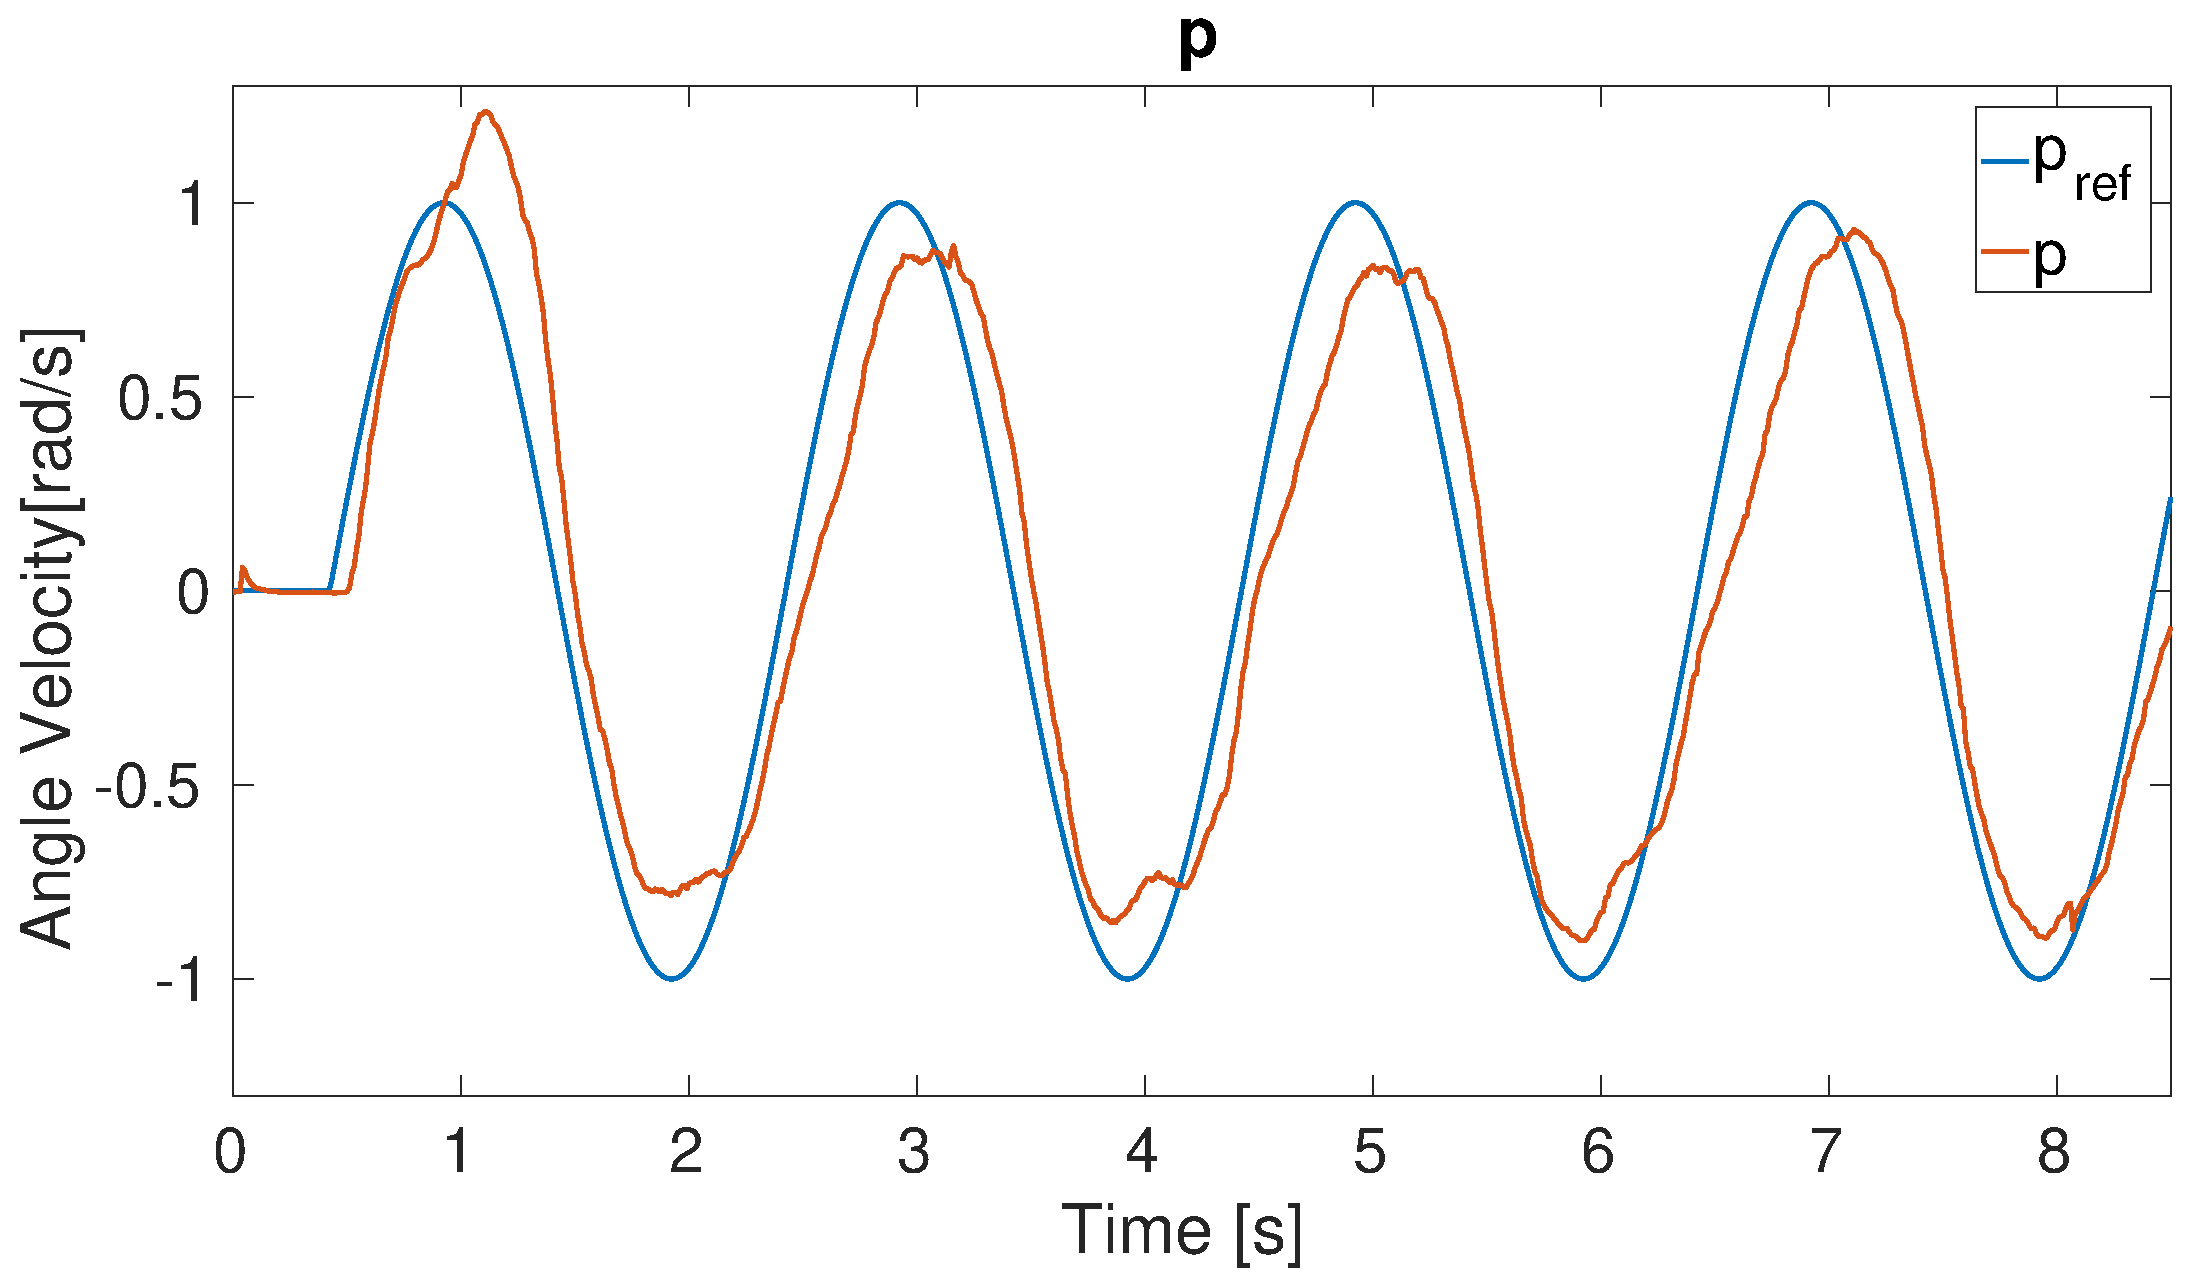
\includegraphics[width=0.4\textwidth]{testSinAllPA1}}
  \qquad
  \subfloat[][\label{fig:simSinAllPRate} Simulated response in $\rollVelocity$.]{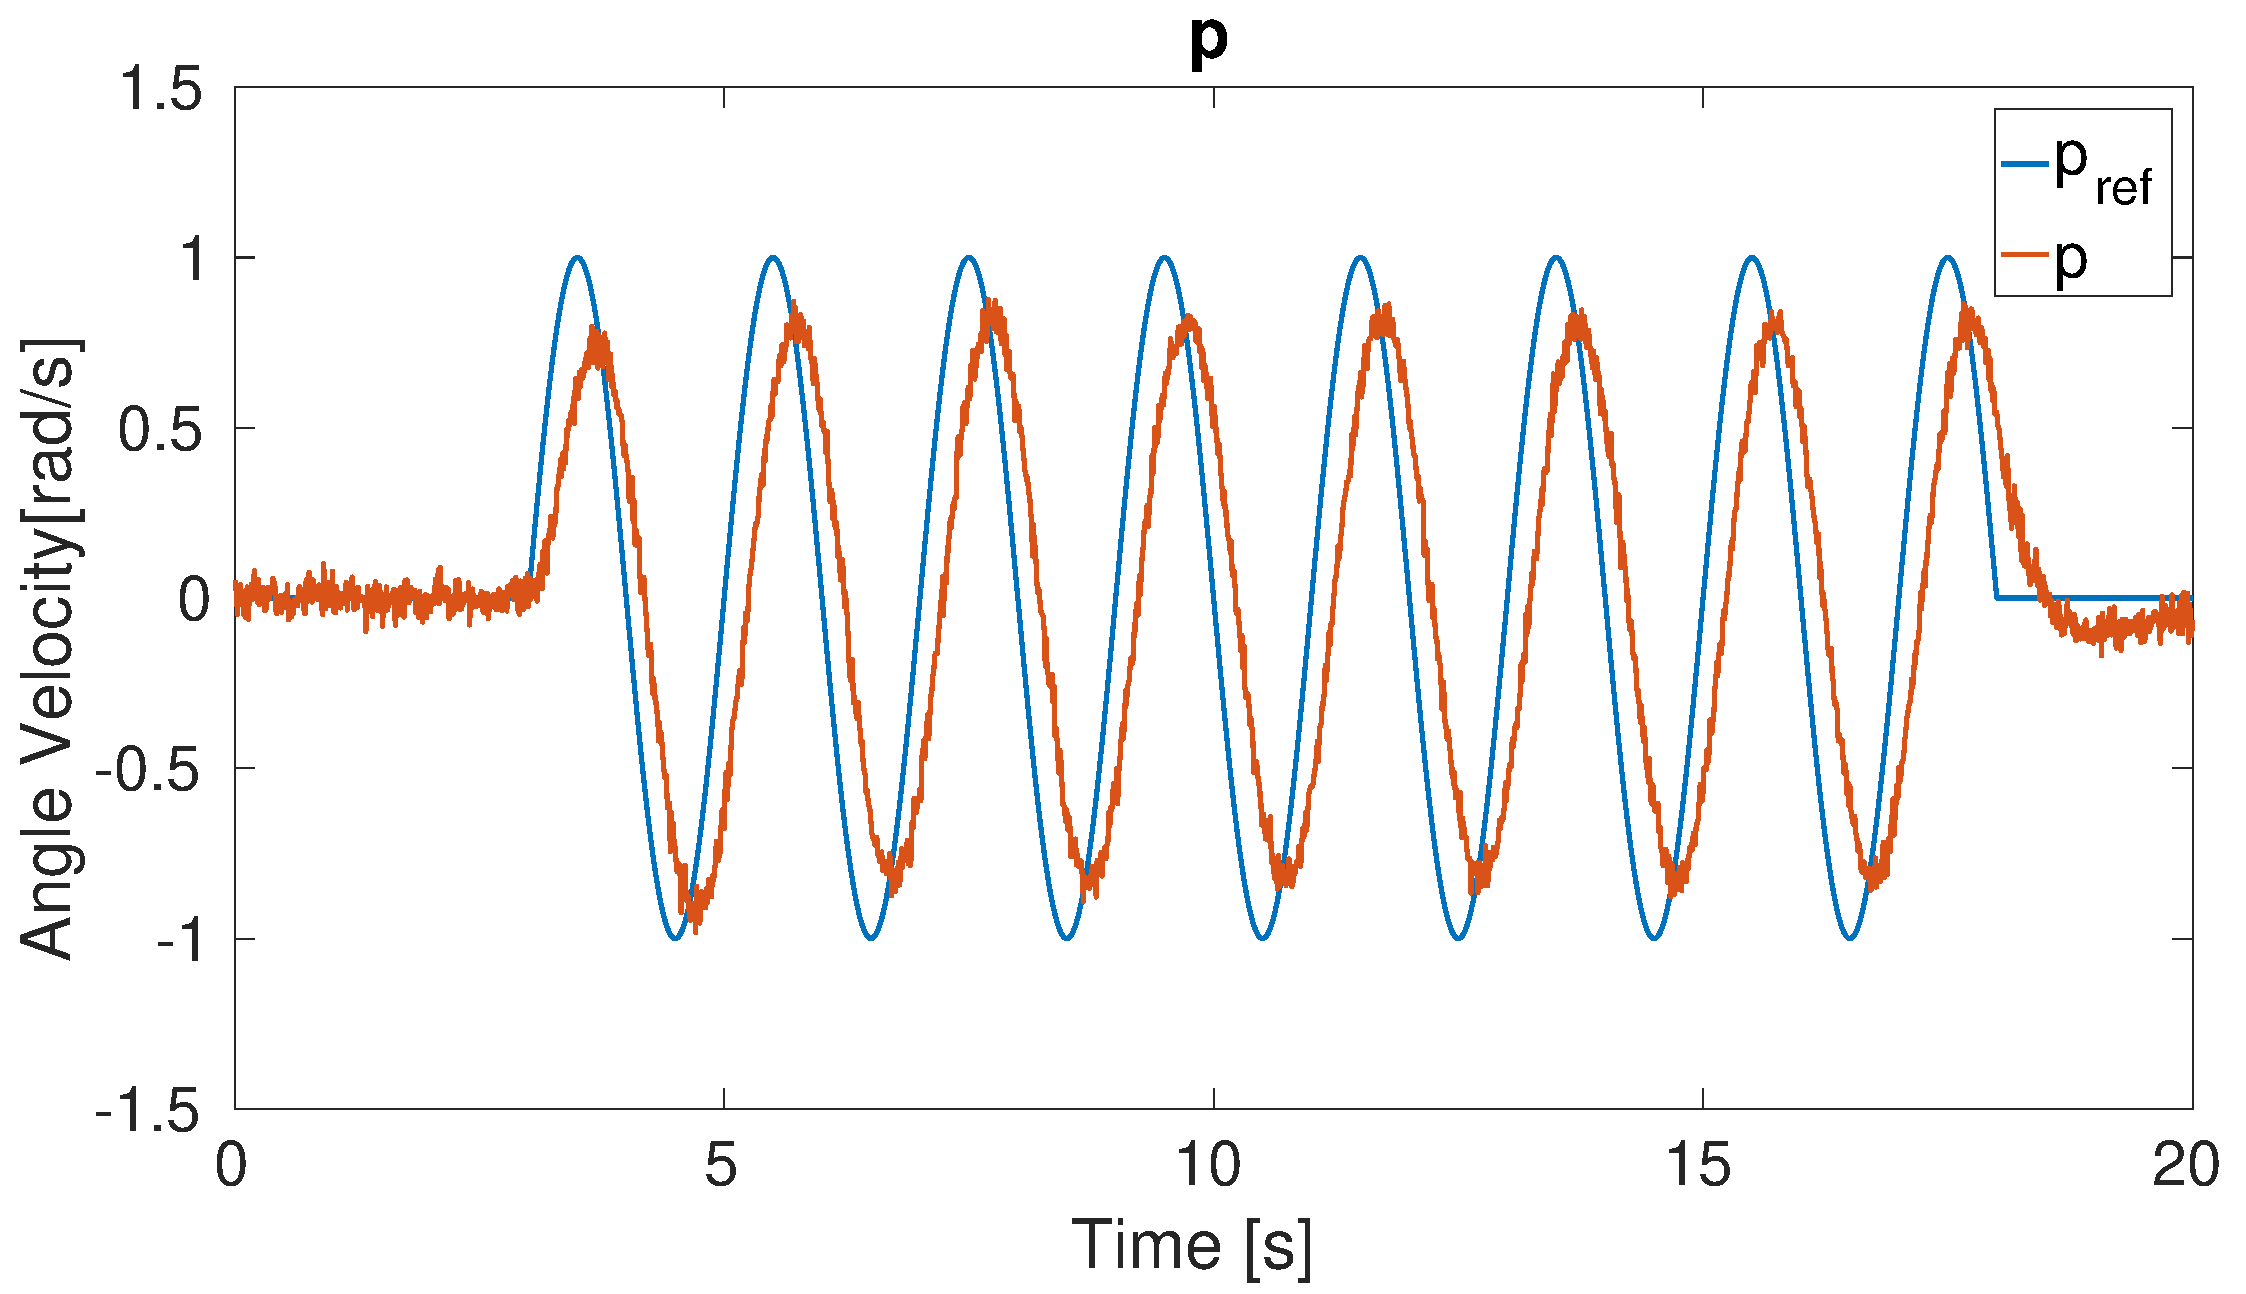
\includegraphics[width=0.4\textwidth]{simSinAllPA1}}
  \qquad
  \subfloat[][\label{fig:testSinAllQRate} Test response in $\pitchVelocity$.]{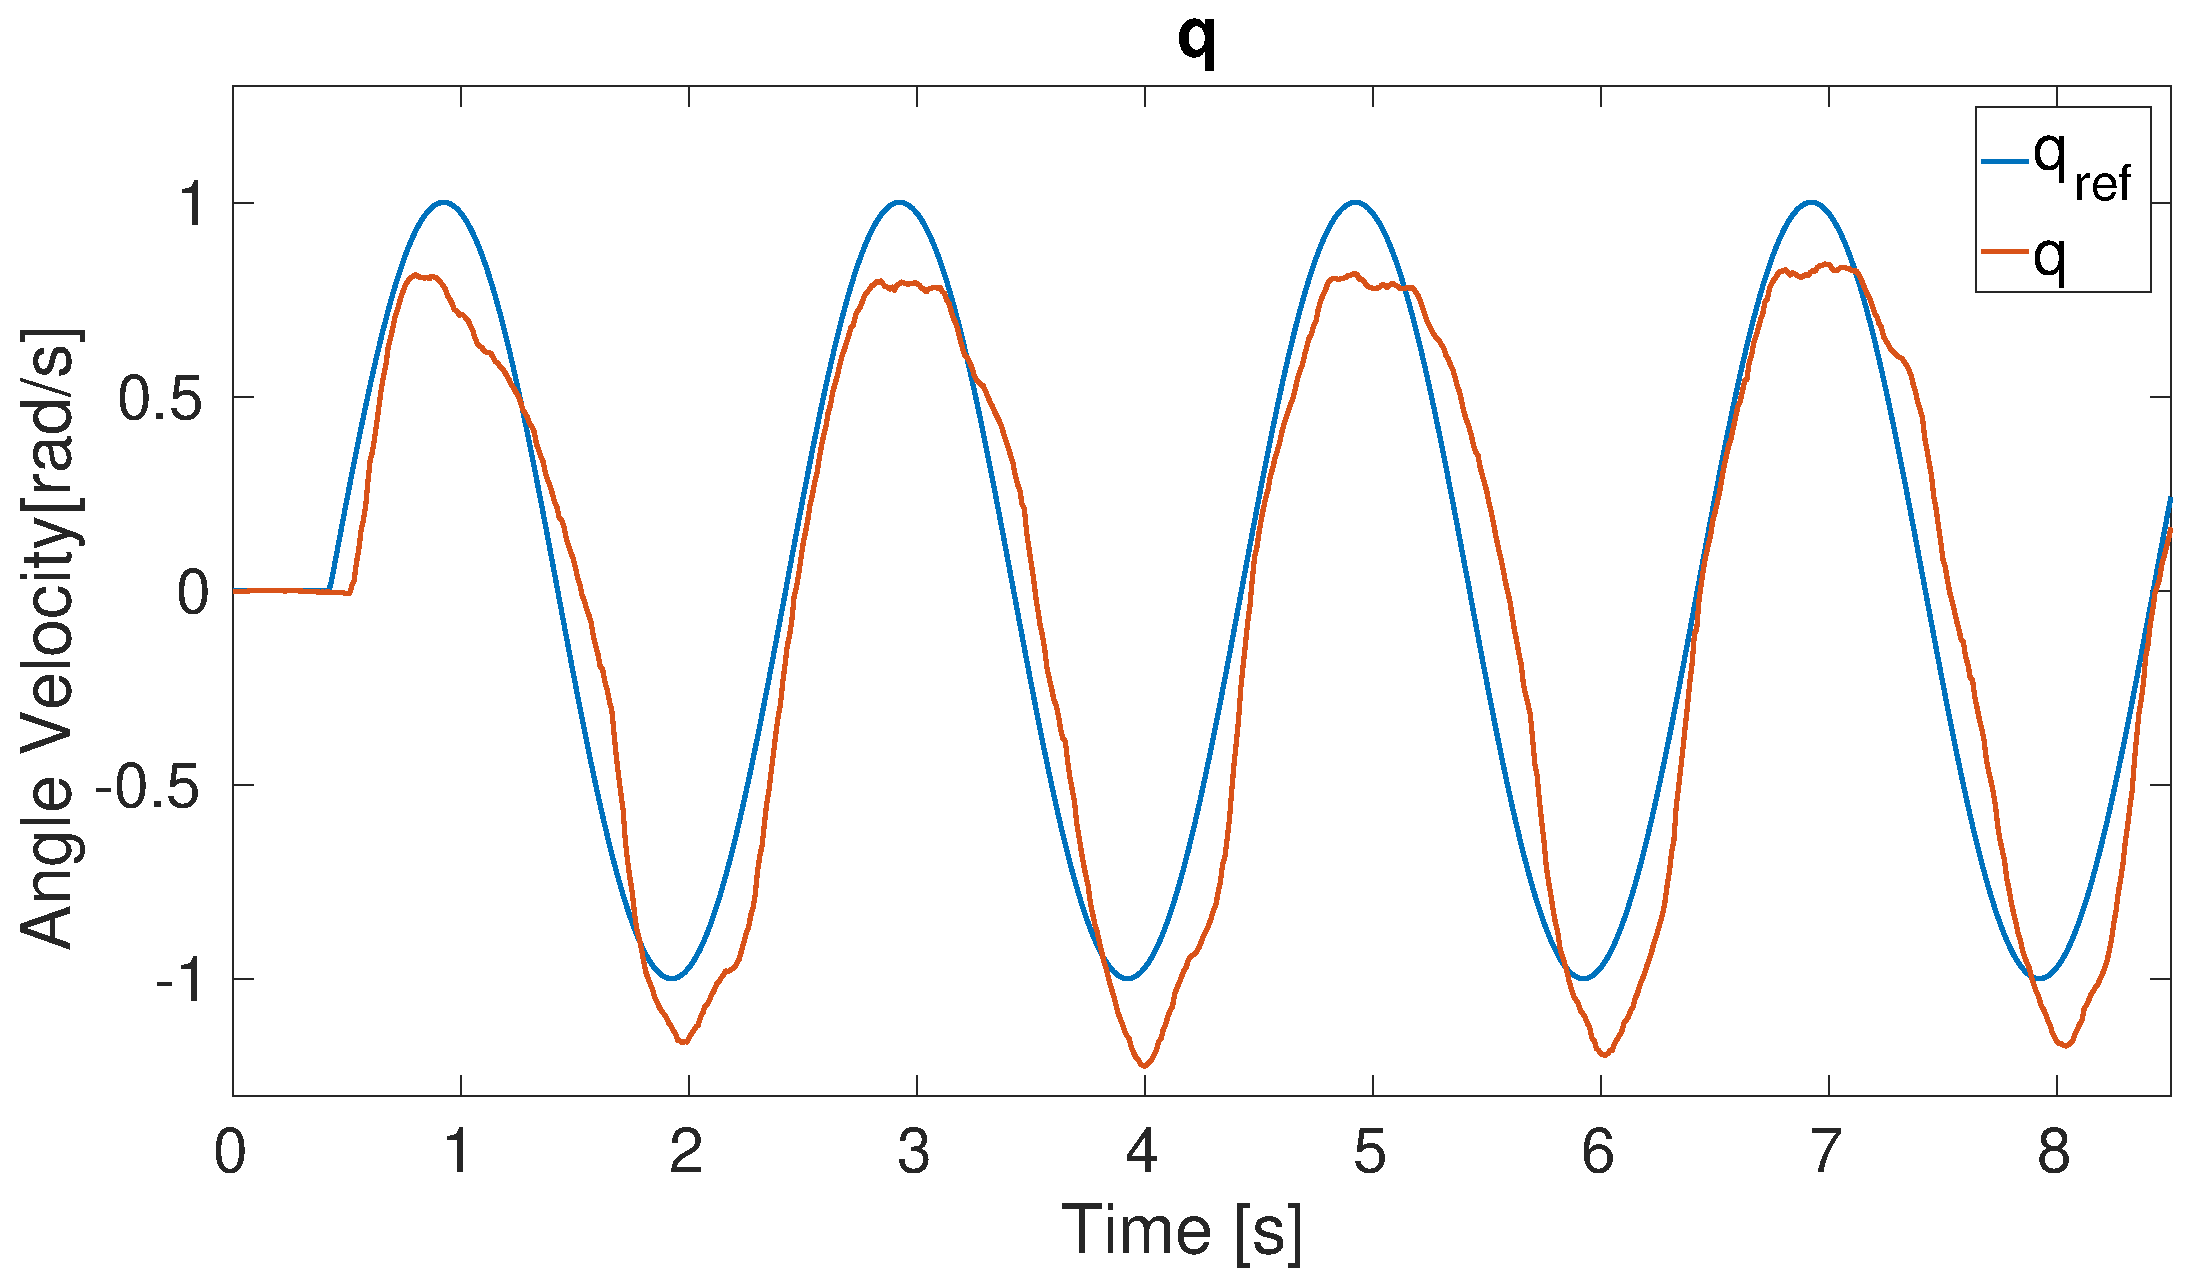
\includegraphics[width=0.4\textwidth]{testSinAllQA1}}
  \qquad
  \subfloat[][\label{fig:simSinAllQRate} Simulated response in $\pitchVelocity$.]{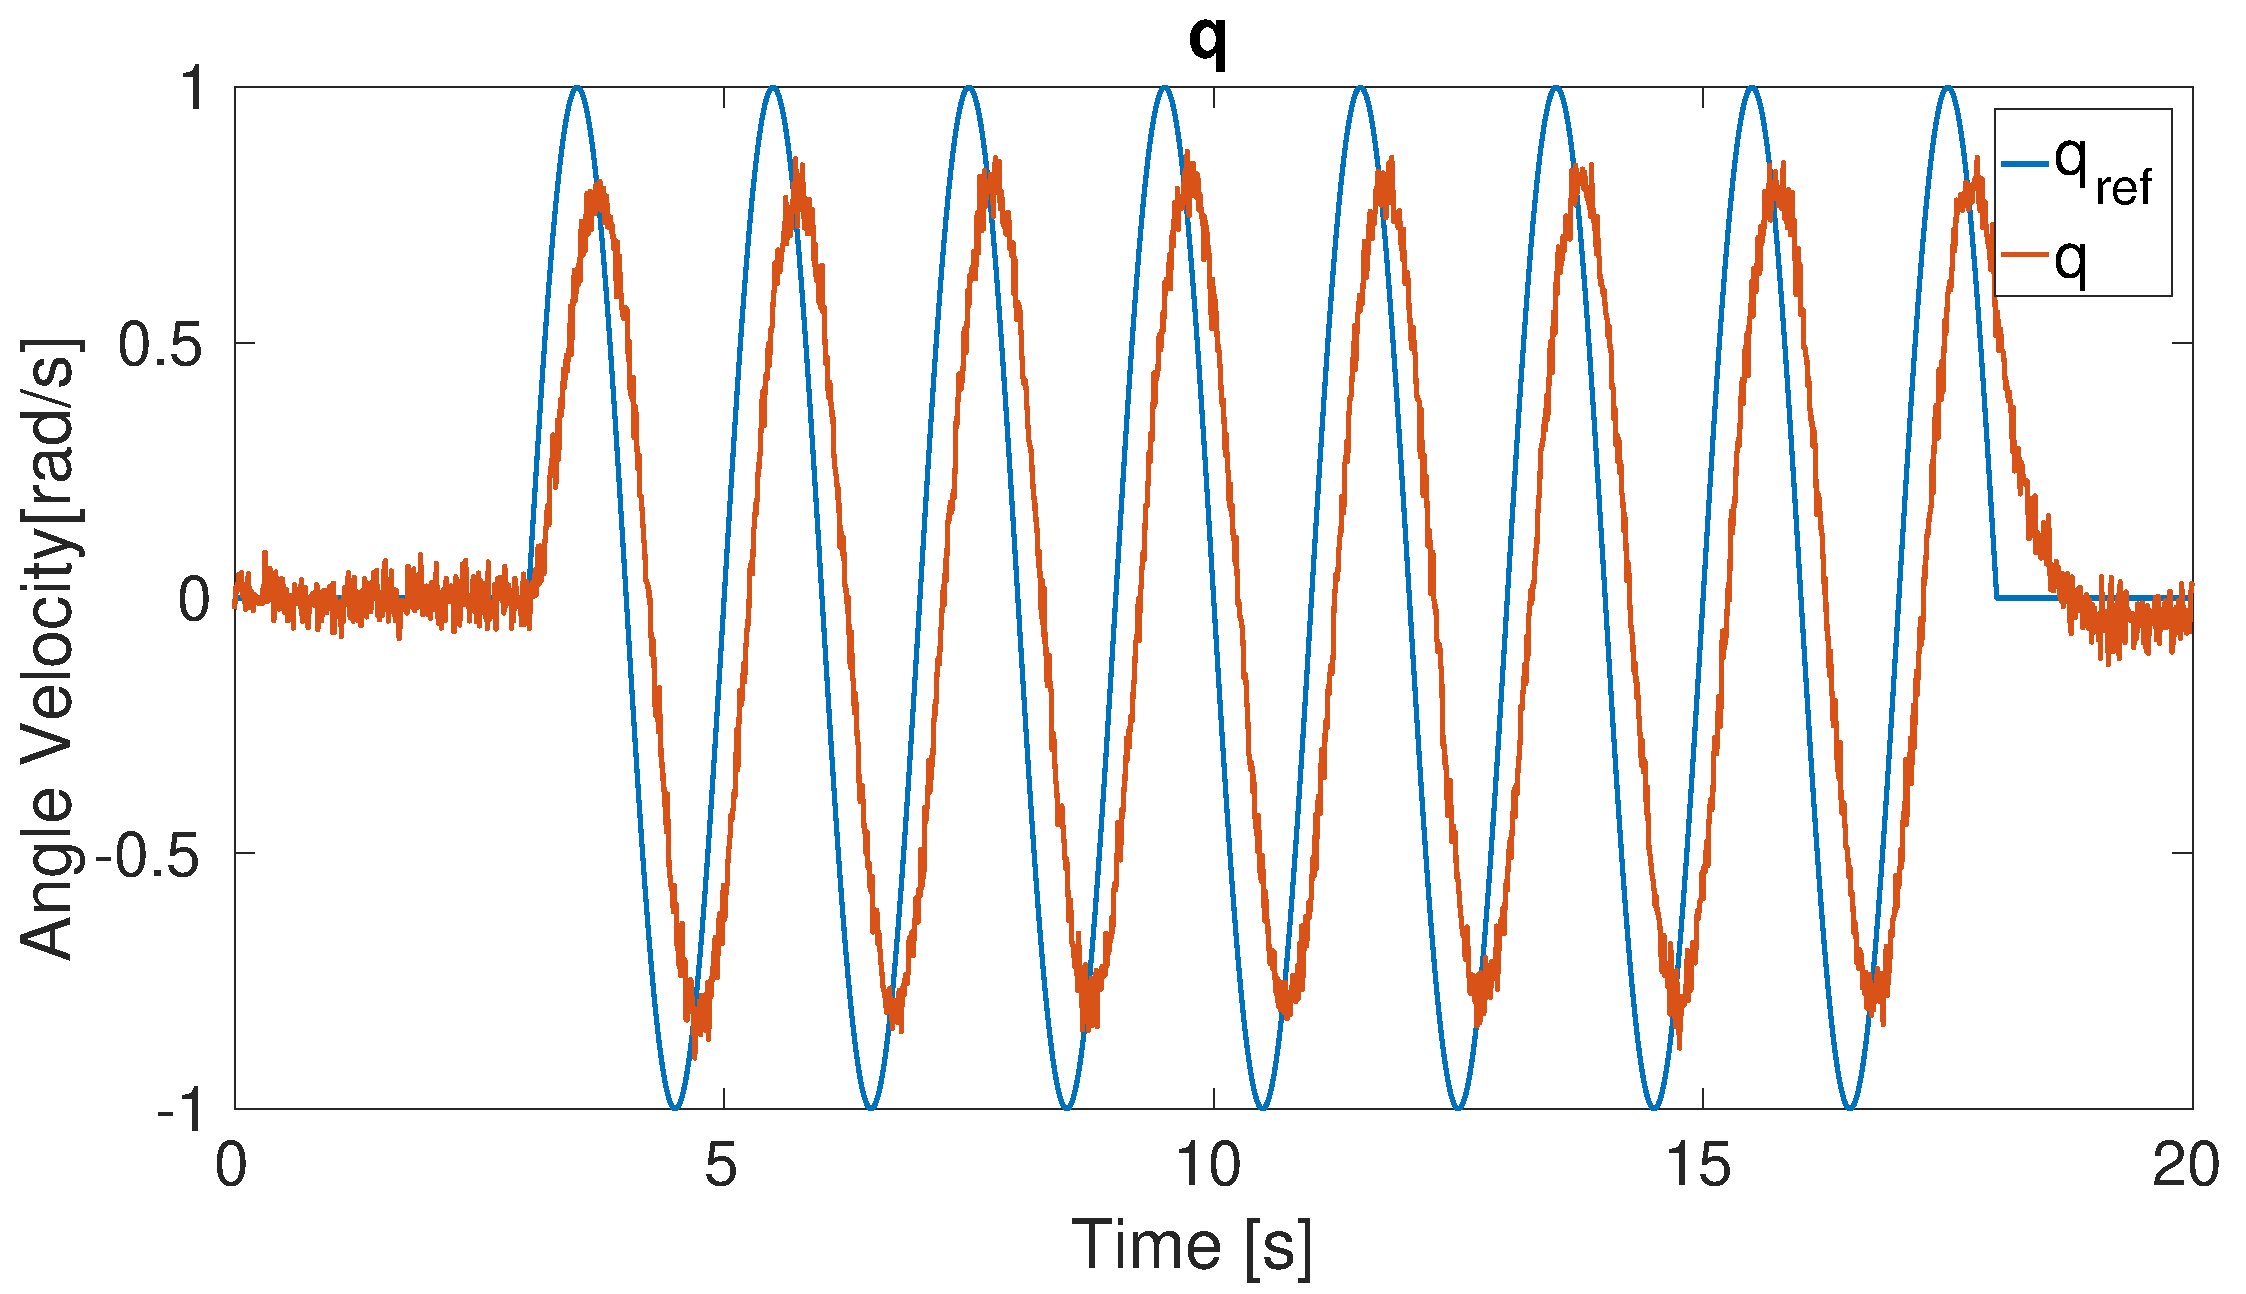
\includegraphics[width=0.4\textwidth]{simSinAllQA1}}
  \qquad
  \subfloat[][\label{fig:testSinAllRRate} Test response in $\yawVelocity$.]{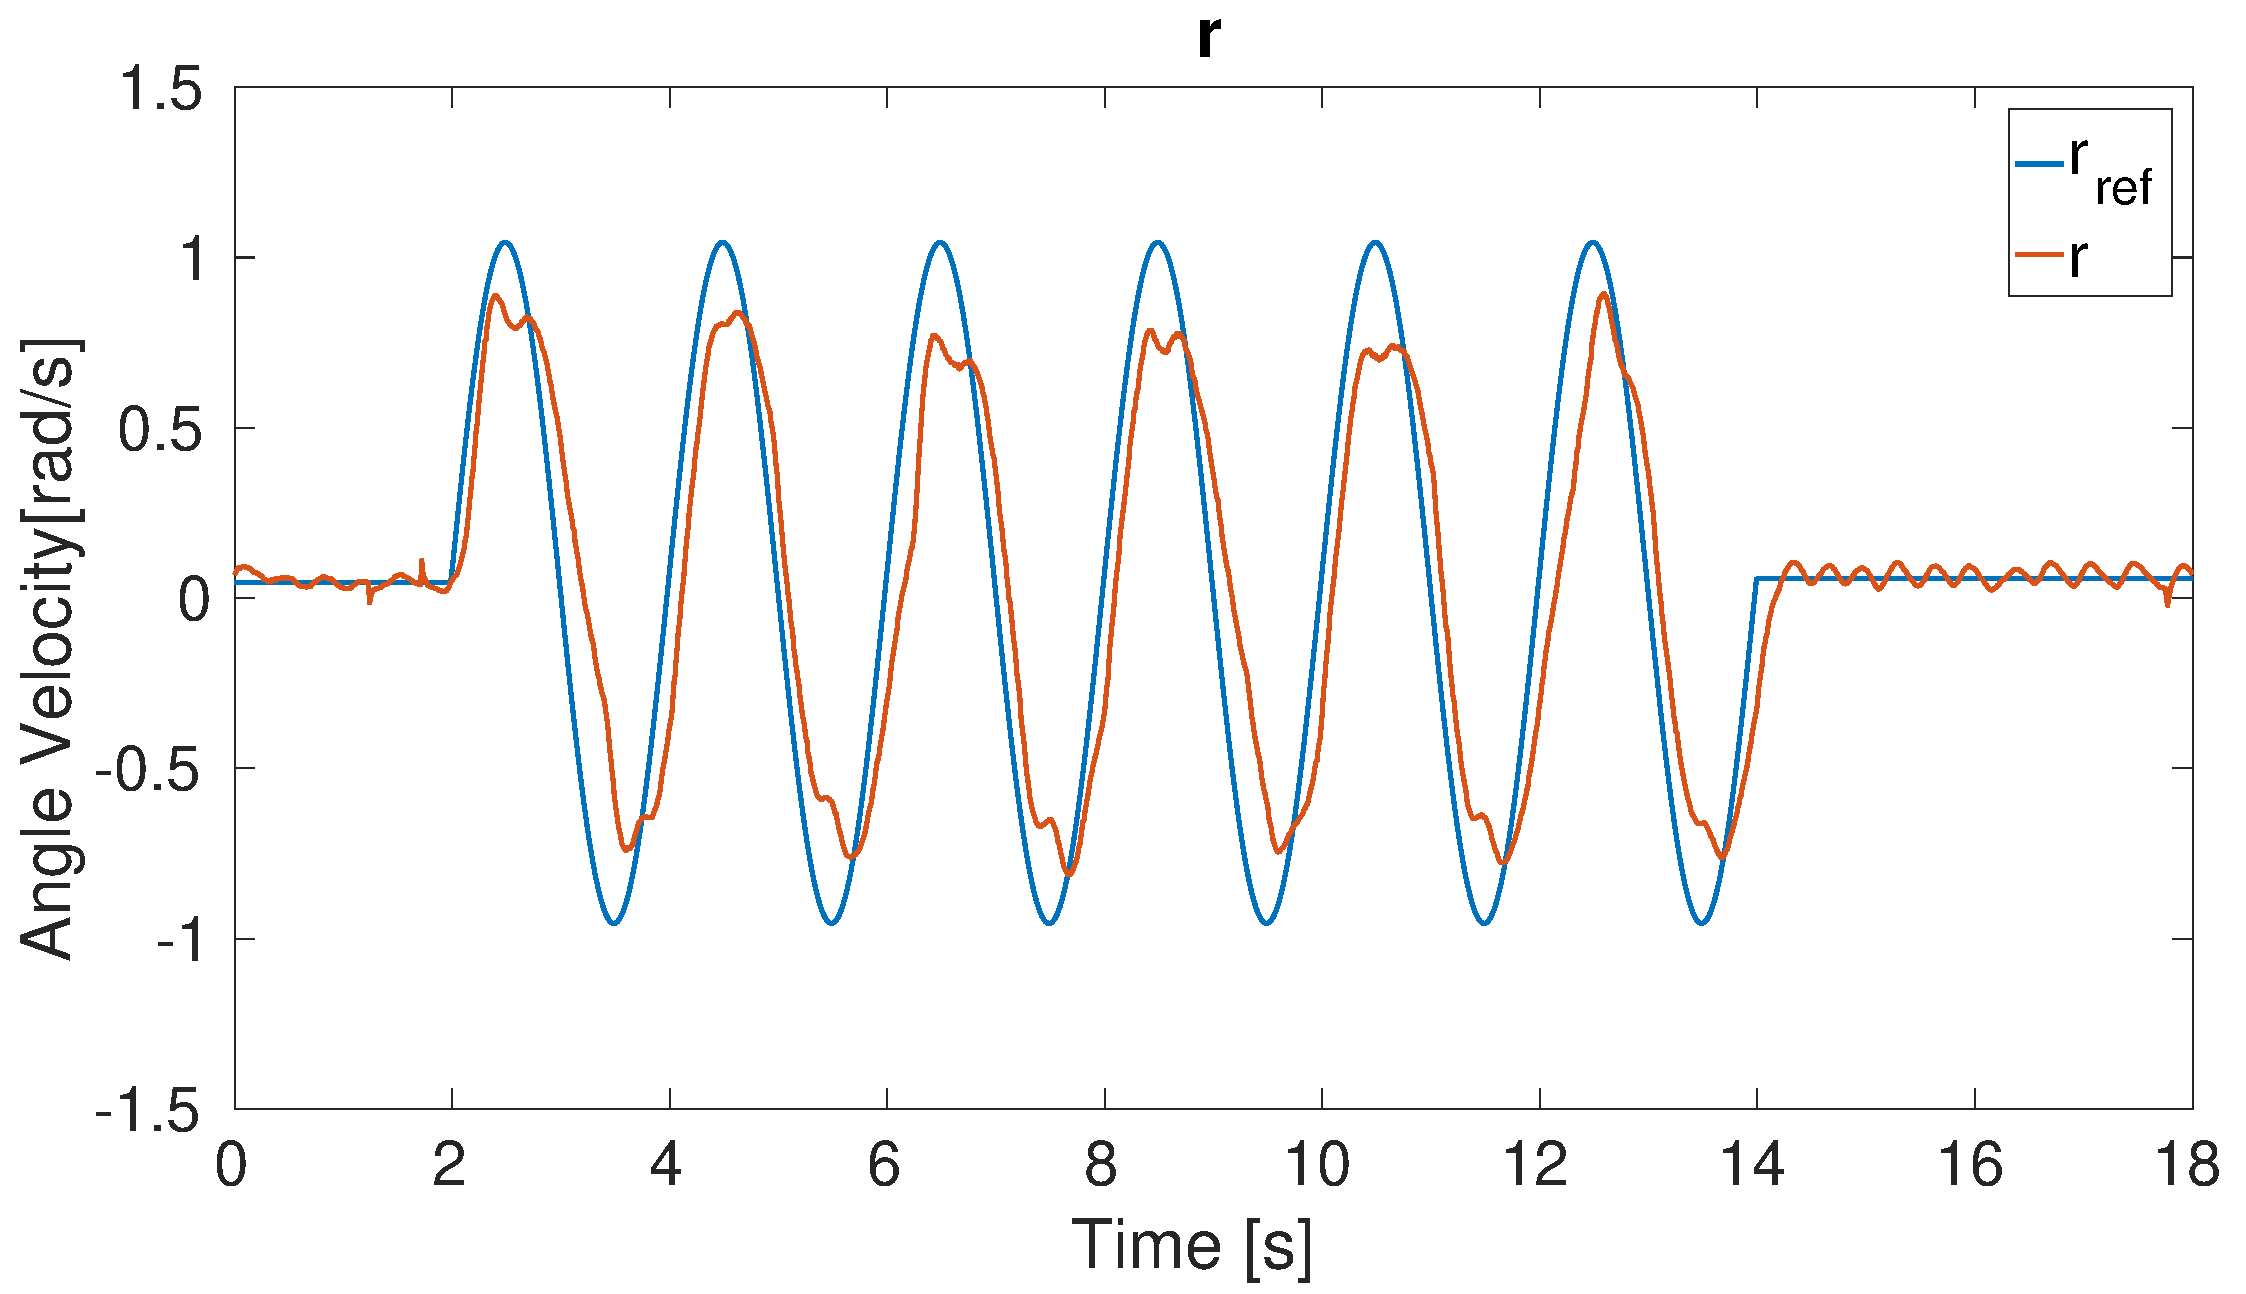
\includegraphics[width=0.4\textwidth]{testSinAllRA1}}
  \qquad
  \subfloat[][\label{fig:simSinAllRRate} Simulated response in $\yawVelocity$.]{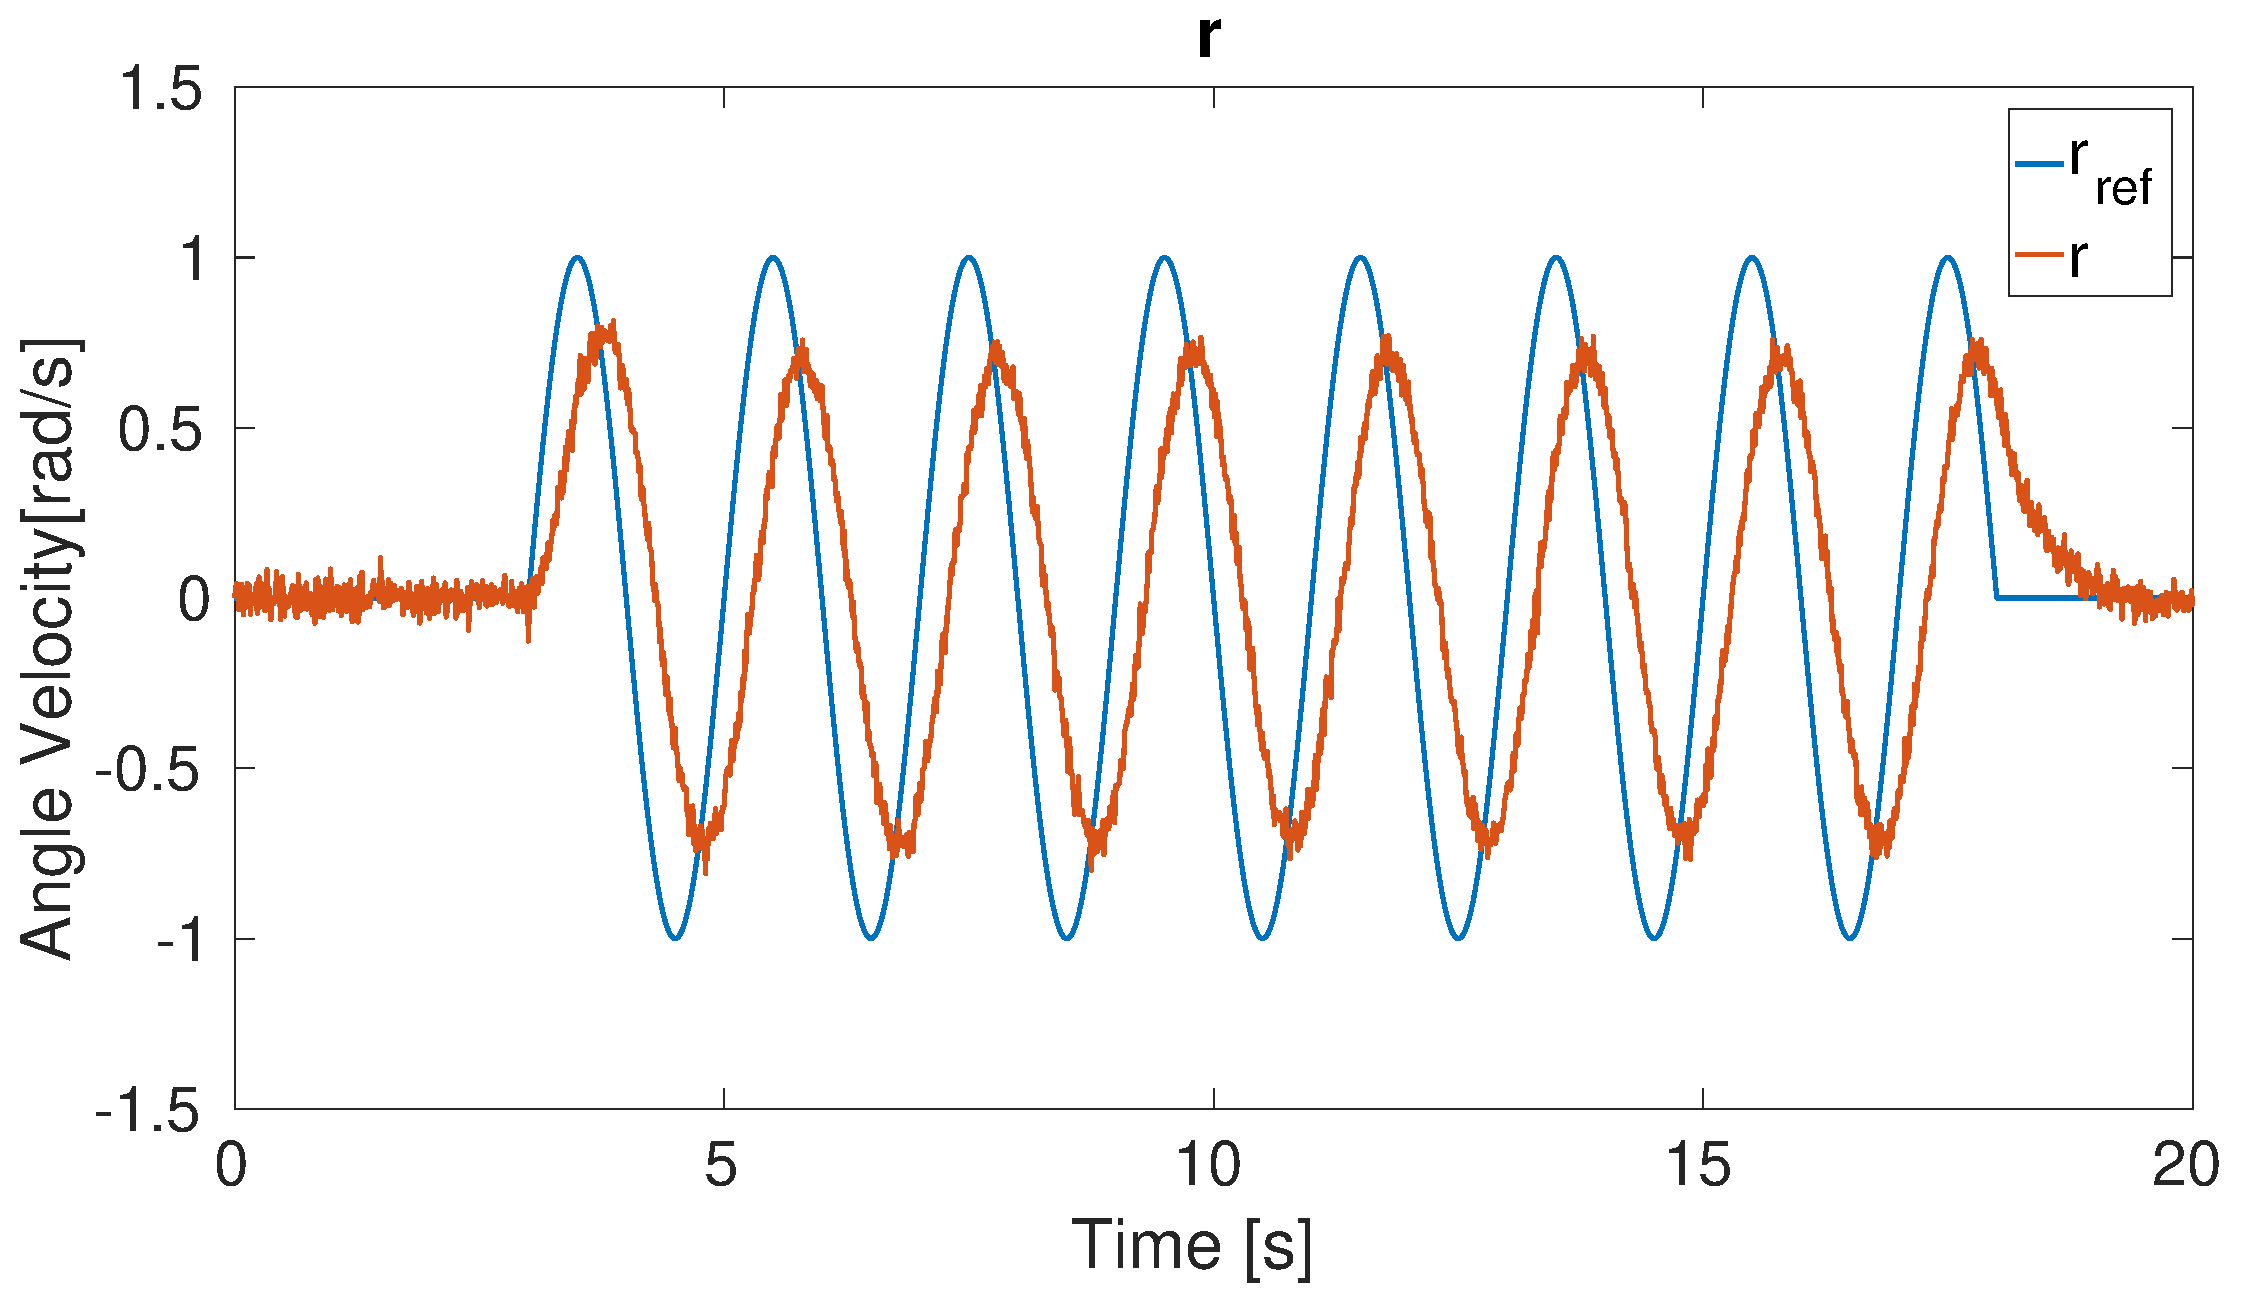
\includegraphics[width=0.4\textwidth]{simSinAllRA1}}
  \caption{\label{fig:SinAllRate}%
  A sine signal with amplitude $1$ and frequency $0.5\ \hertz$ was applied in all angular velocities at the same time while using the angular velocity controller.}
\end{figure}

A sine signal was also applied to all angular velocities while using the angular velocity controller. The results can be seen in \Figureref{fig:SinAllRate}. During the field tests all the angular velocities followed the reference signals well, except for some overshoots and undershoots. The simulated test followed a general sine form but the reference amplitude was not reached and a phase shift could be noted.

%%%%%%%%%%%%%%%%%%%%%%%%%%%Depth%%%%%%%%%%%%%%%%
\begin{figure}[tbp]
  \centering
  \subfloat[][\label{fig:testStepD1} A smooth step applied in $\zPosition$.]{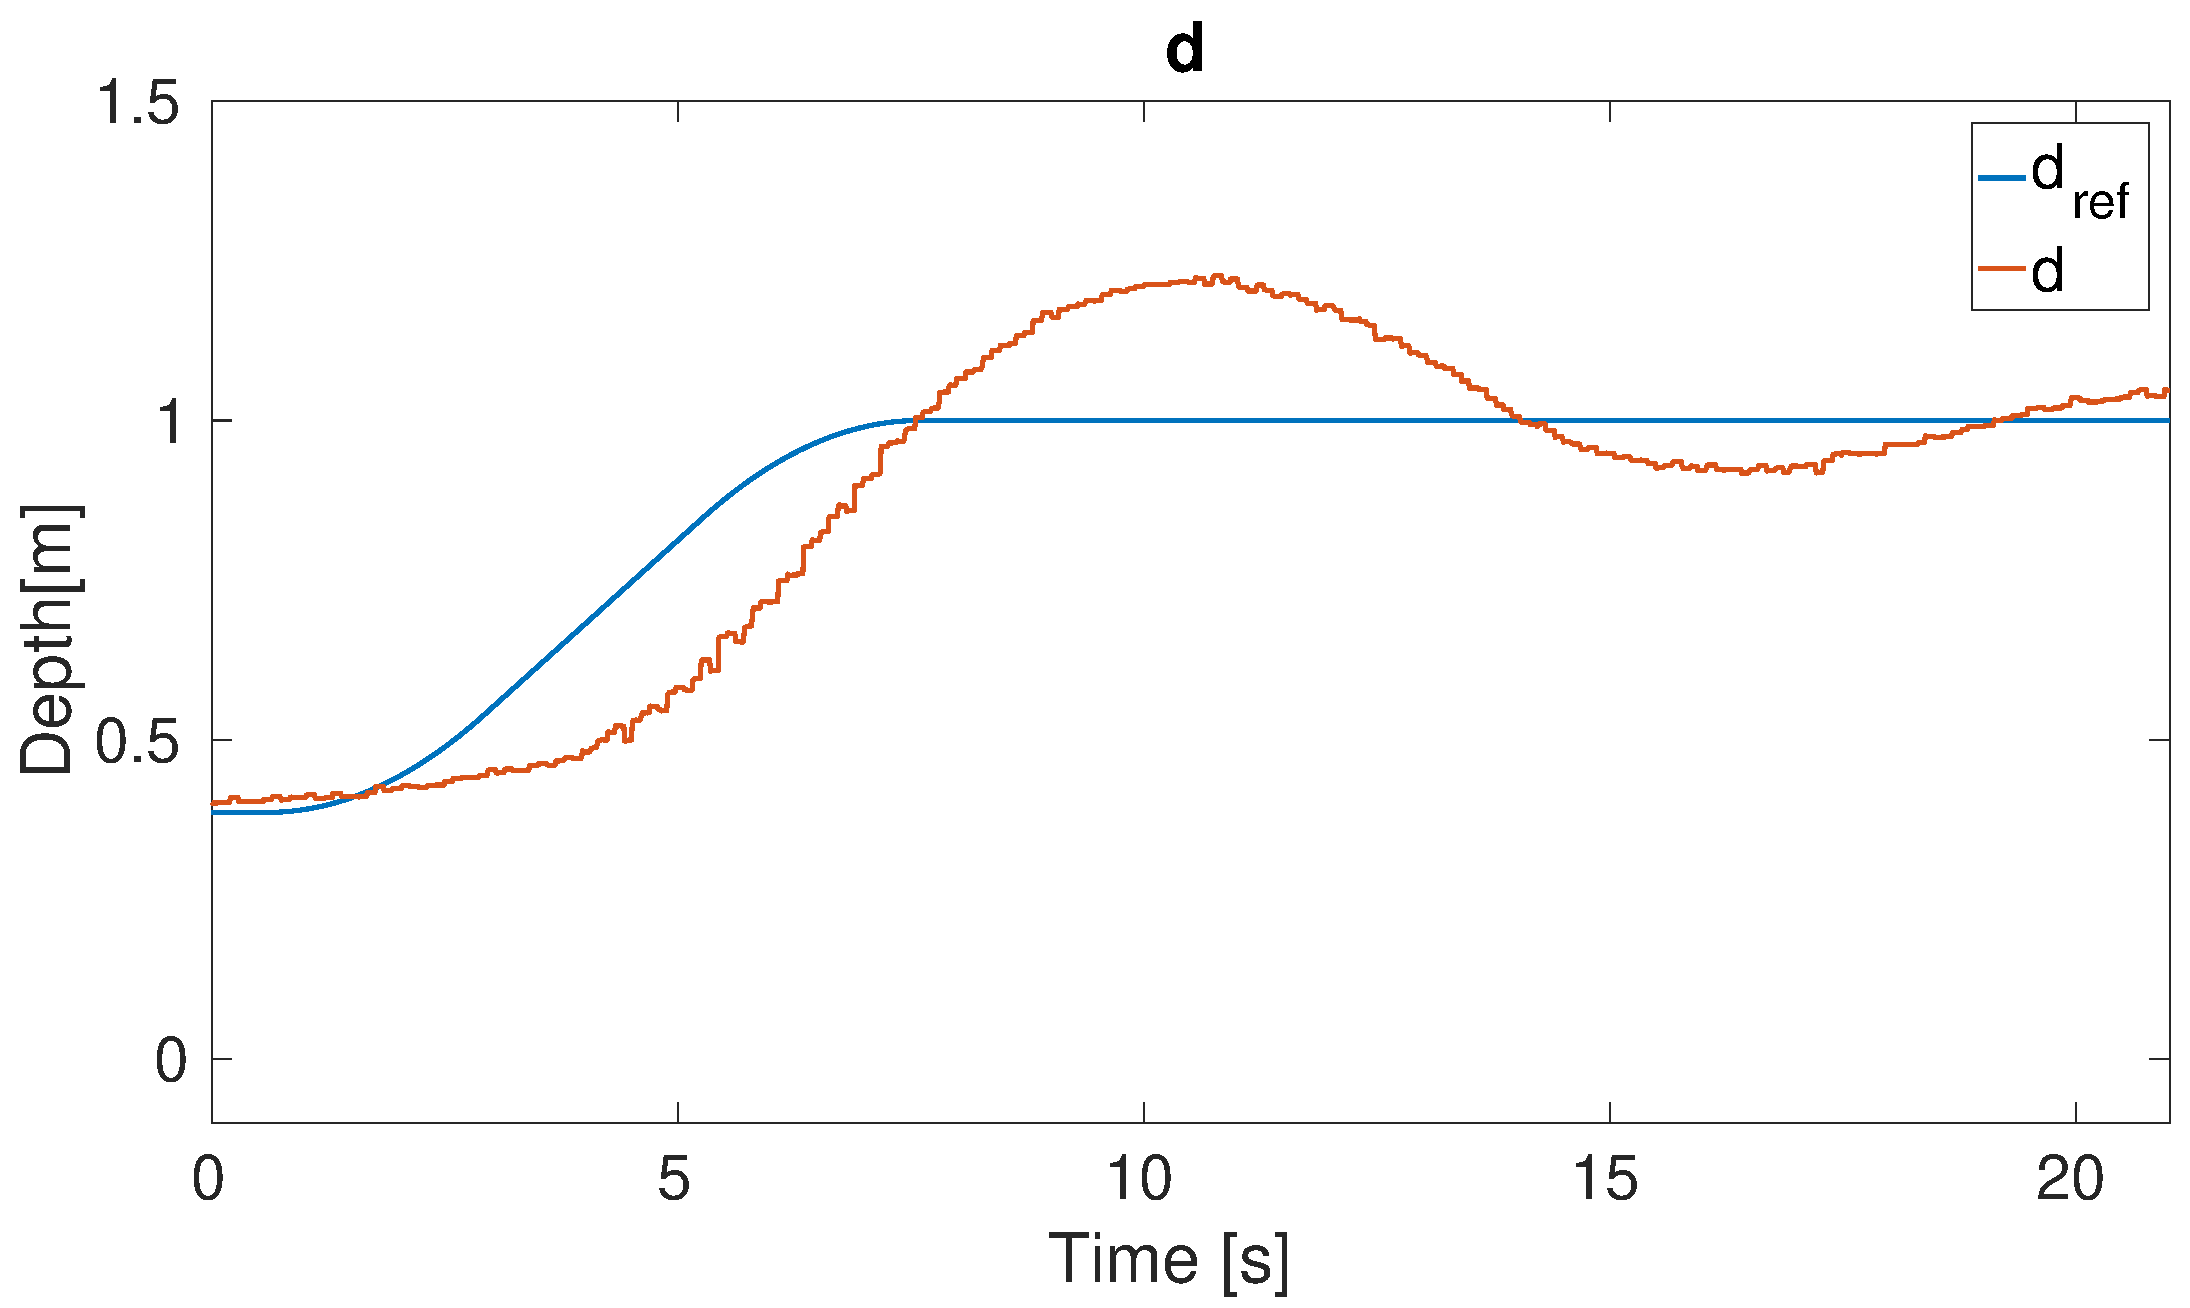
\includegraphics[width=0.4\textwidth]{testStepDepth3e10a1}}
  \qquad
  \subfloat[][\label{fig:testStepD2} A step applied in $\zPosition$.]{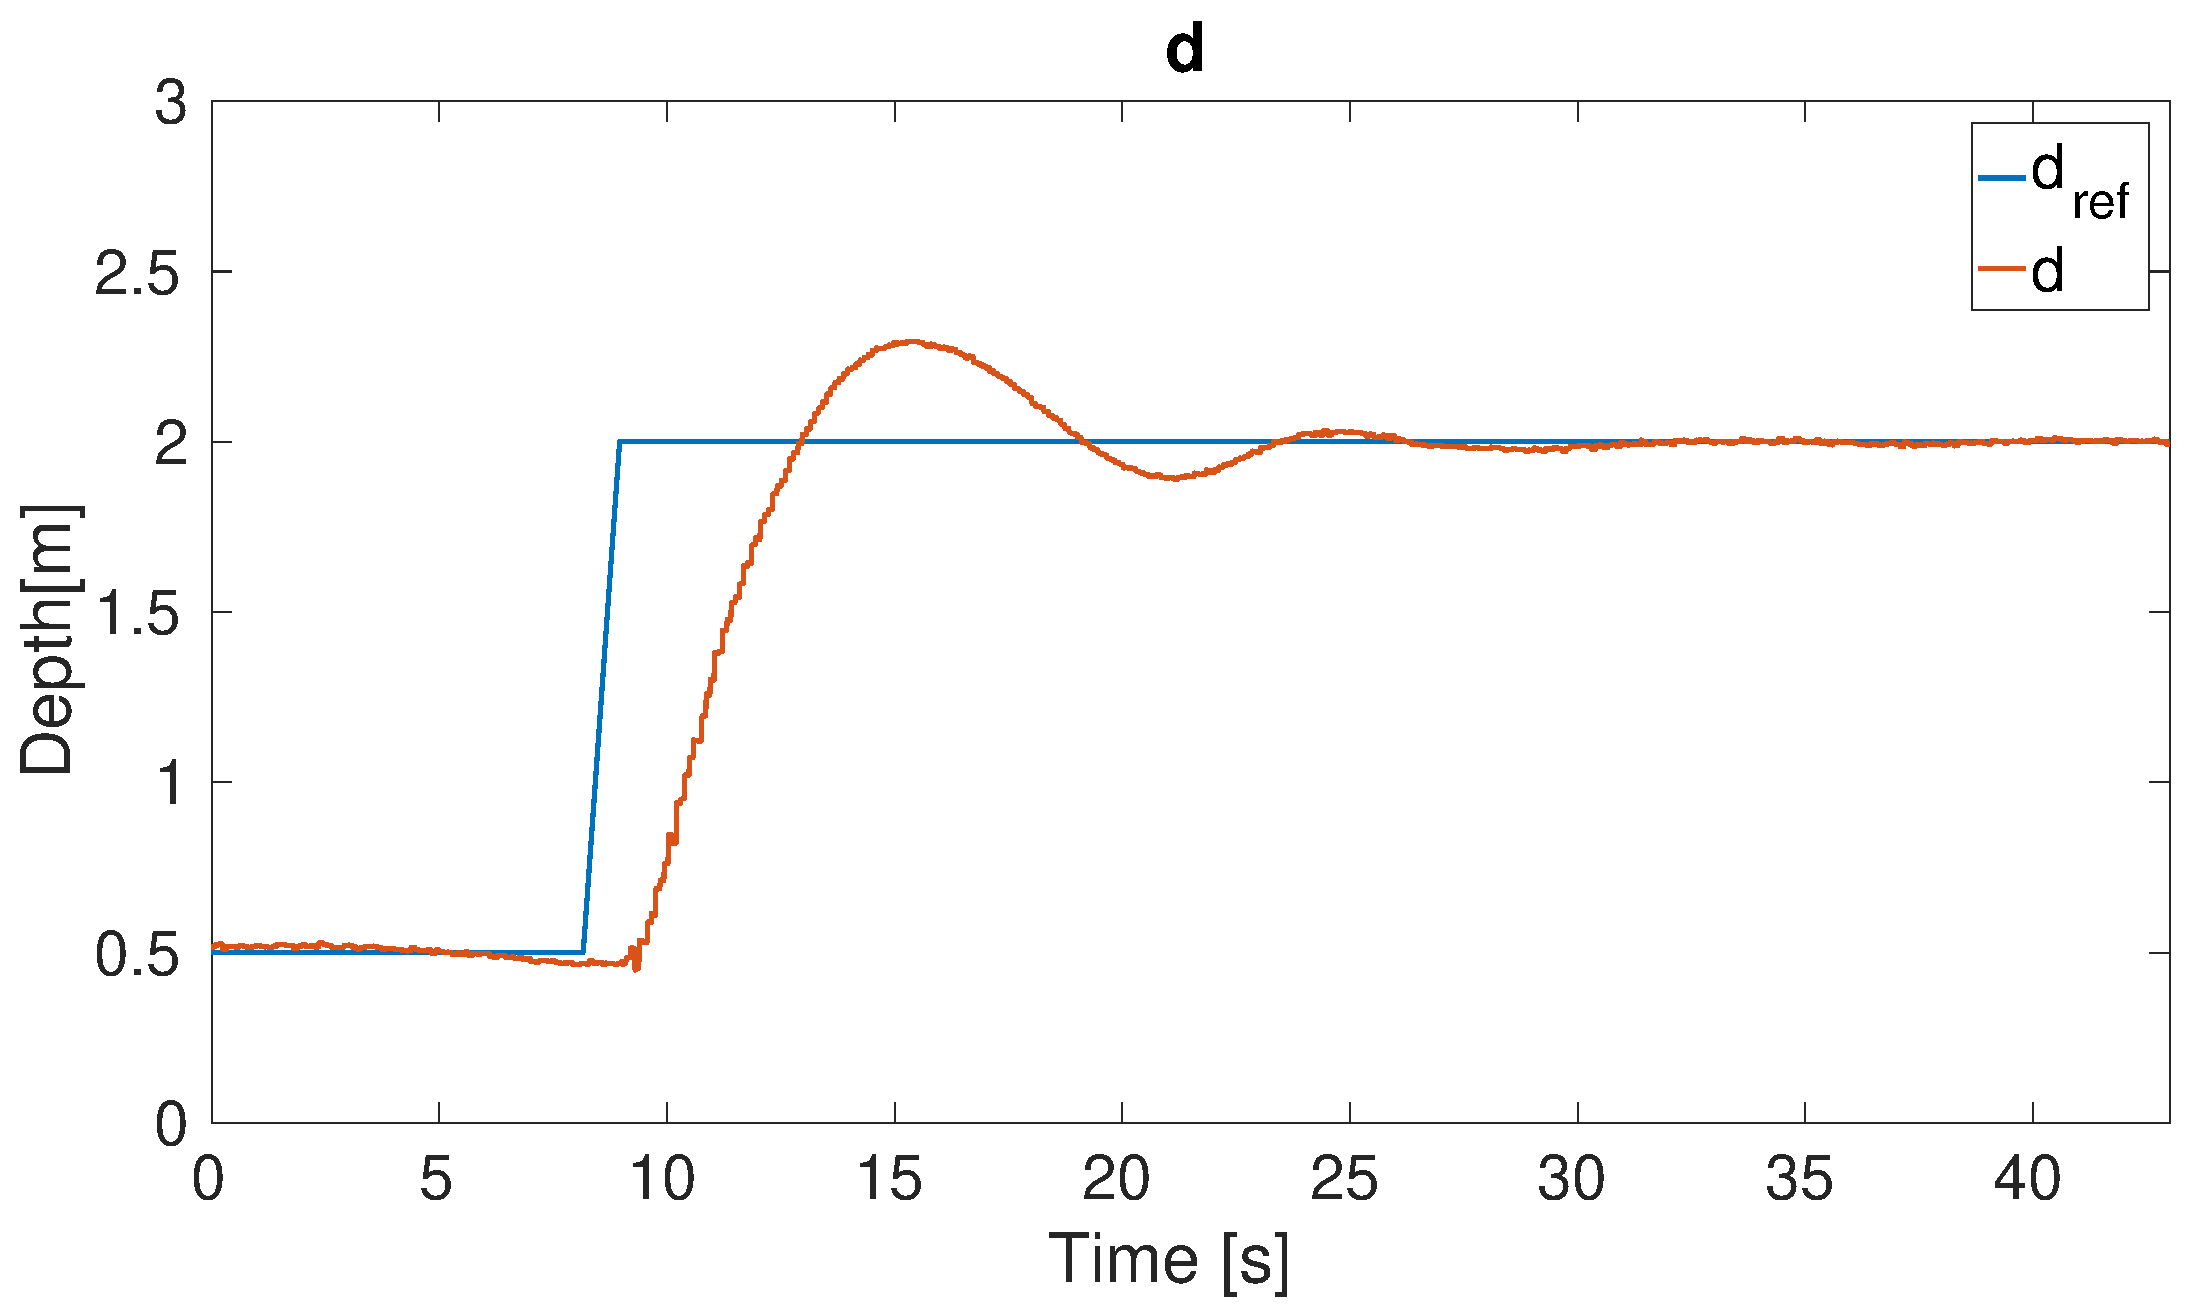
\includegraphics[width=0.4\textwidth]{testConstantD1}}
  \caption{\label{fig:StepD}%
    Steps applied to $\zPosition$. A smooth step from $0.4\ \meter$ to $1\ \meter$ is shown in (a) and a step from $0.5 \meter$ to $2 \meter$ is shown in (b).}
\end{figure}

\Figureref{fig:StepD} shows a smooth step from $0.4\ \meter$ to $1\ \meter$ and a step from $0.5\ \meter$ to $2\ \meter$. A delay in the response can be seen and overshoots of approximately 0.2.

%%%%%%%%%%%%%%%%%%%%%%%%%%%%%%%%%%%%%%%%
\section{Discussion}\label{sec:controlDiscussion}
Due to problems during implementation of the controllers, they were not as well tuned as they could have been. This can be seen in the results since large steady-state errors were acquired during the tests. The \abbrPID -parameters were trimmed in simulation before live test but the feedback used in simulations was too strong for live tests. The parameters in the feedback and the linearising control law both had to be scaled down to achieve a stable system. Since the \abbrROV is a non-linear and stable system, compensating for non-linearities run the risk of producing a non-linear and unstable system. This is further illustrated in \Exampleref{ex:exact}. We believe such an over compensation was what caused most of the initial problems during controller tests. This idea is further strengthened by the fact that the controller instability diminished when the parameters in the linearising control law were scaled down.
\begin{example}\label{ex:exact}
Consider the non-linear system
\begin{equation}\label{eq:exampleSys}
\begin{bmatrix}
\dot{x}_1\\
\dot{x}_2
\end{bmatrix}=
\begin{bmatrix}
x_2\\
-a x_1 - b x_2\abs{x_2} + u
\end{bmatrix}
\end{equation}
Using feedback linearisation, the ideal case would be to use the control law 
\begin{equation}\label{eq:exampleLaw}
u = a x_1 +b x_2\abs{x_2} + \bar{u}
\end{equation} which would yield the linear system
\begin{equation}
\begin{bmatrix}
\dot{x}_1\\
\dot{x}_2
\end{bmatrix}=
\begin{bmatrix}
x_2\\
\bar{u}
\end{bmatrix}
\end{equation}
Here, $\bar{u}$ can be used to achieve the desired dynamics, for example, using a \abbrPID-controller. 

In practice however, both $a$ and $b$ have to be estimated with $\hat{a}$ and $\hat{b}$. Using the estimated values $\hat{a}$ and $\hat{b}$ in \eqref{eq:exampleLaw} gives 
\begin{equation}
\begin{bmatrix}
\dot{x}_1\\
\dot{x}_2
\end{bmatrix}=
\begin{bmatrix}
x_2\\
\tilde{a} x_1 + \tilde{b} x_2\abs{x_2} +\bar{u}
\end{bmatrix}
\end{equation}
with $\tilde{a}=\hat{a}-a$ and $\tilde{b}=\hat{b}-b$.

If $\hat{a}$ and $\hat{b}$ are estimated such that $\tilde{a} > 0$ and $\tilde{b} > 0$,
the control law has created an unstable non-linear system. The instability can nevertheless be compensated for by 
applying a strong enough feedback using $\bar{u}$. But a strong feedback is often undesirable since using a stronger control signal means that the system will use more energy. Furthermore, a large control signal is not always possible since $u$ might be saturated.  
\end{example}

Additional problems were encountered during tuning of the attitude \abbrPID using feedback linearisation. The core of the problem was that regardless of the strength of the feedback the \abbrROV never stabilised around the desired references. The result from an attempt to stabilise the \abbrROV using the attitude controller can be seen in \Figureref{fig:ExactLinAttitude}. This problem might originate from bad magnetometer readings, which fluctuated when the \abbrROV engaged its thrusters. It is suspected that such fluctuations in magnetic field strength may cause rapid changes in the estimated quaternions and angular velocities. This would in turn lead to problems when computing \eqref{eq:anLaw} in the feedback linearisation. %The problem could also be caused by badly estimated parameters from \Chapterref{cha:modelling}. The likelihood of the problem lying with the parameters is strengthened by the fact that the estimated model parameters had to be scaled down in the exact linearisation to get the rate controller to be stable. 

\begin{figure}
\centering
  \subfloat[][\label{fig:testExactAttitudeRoll} The feedback linearisation in $\rollAngle$.]{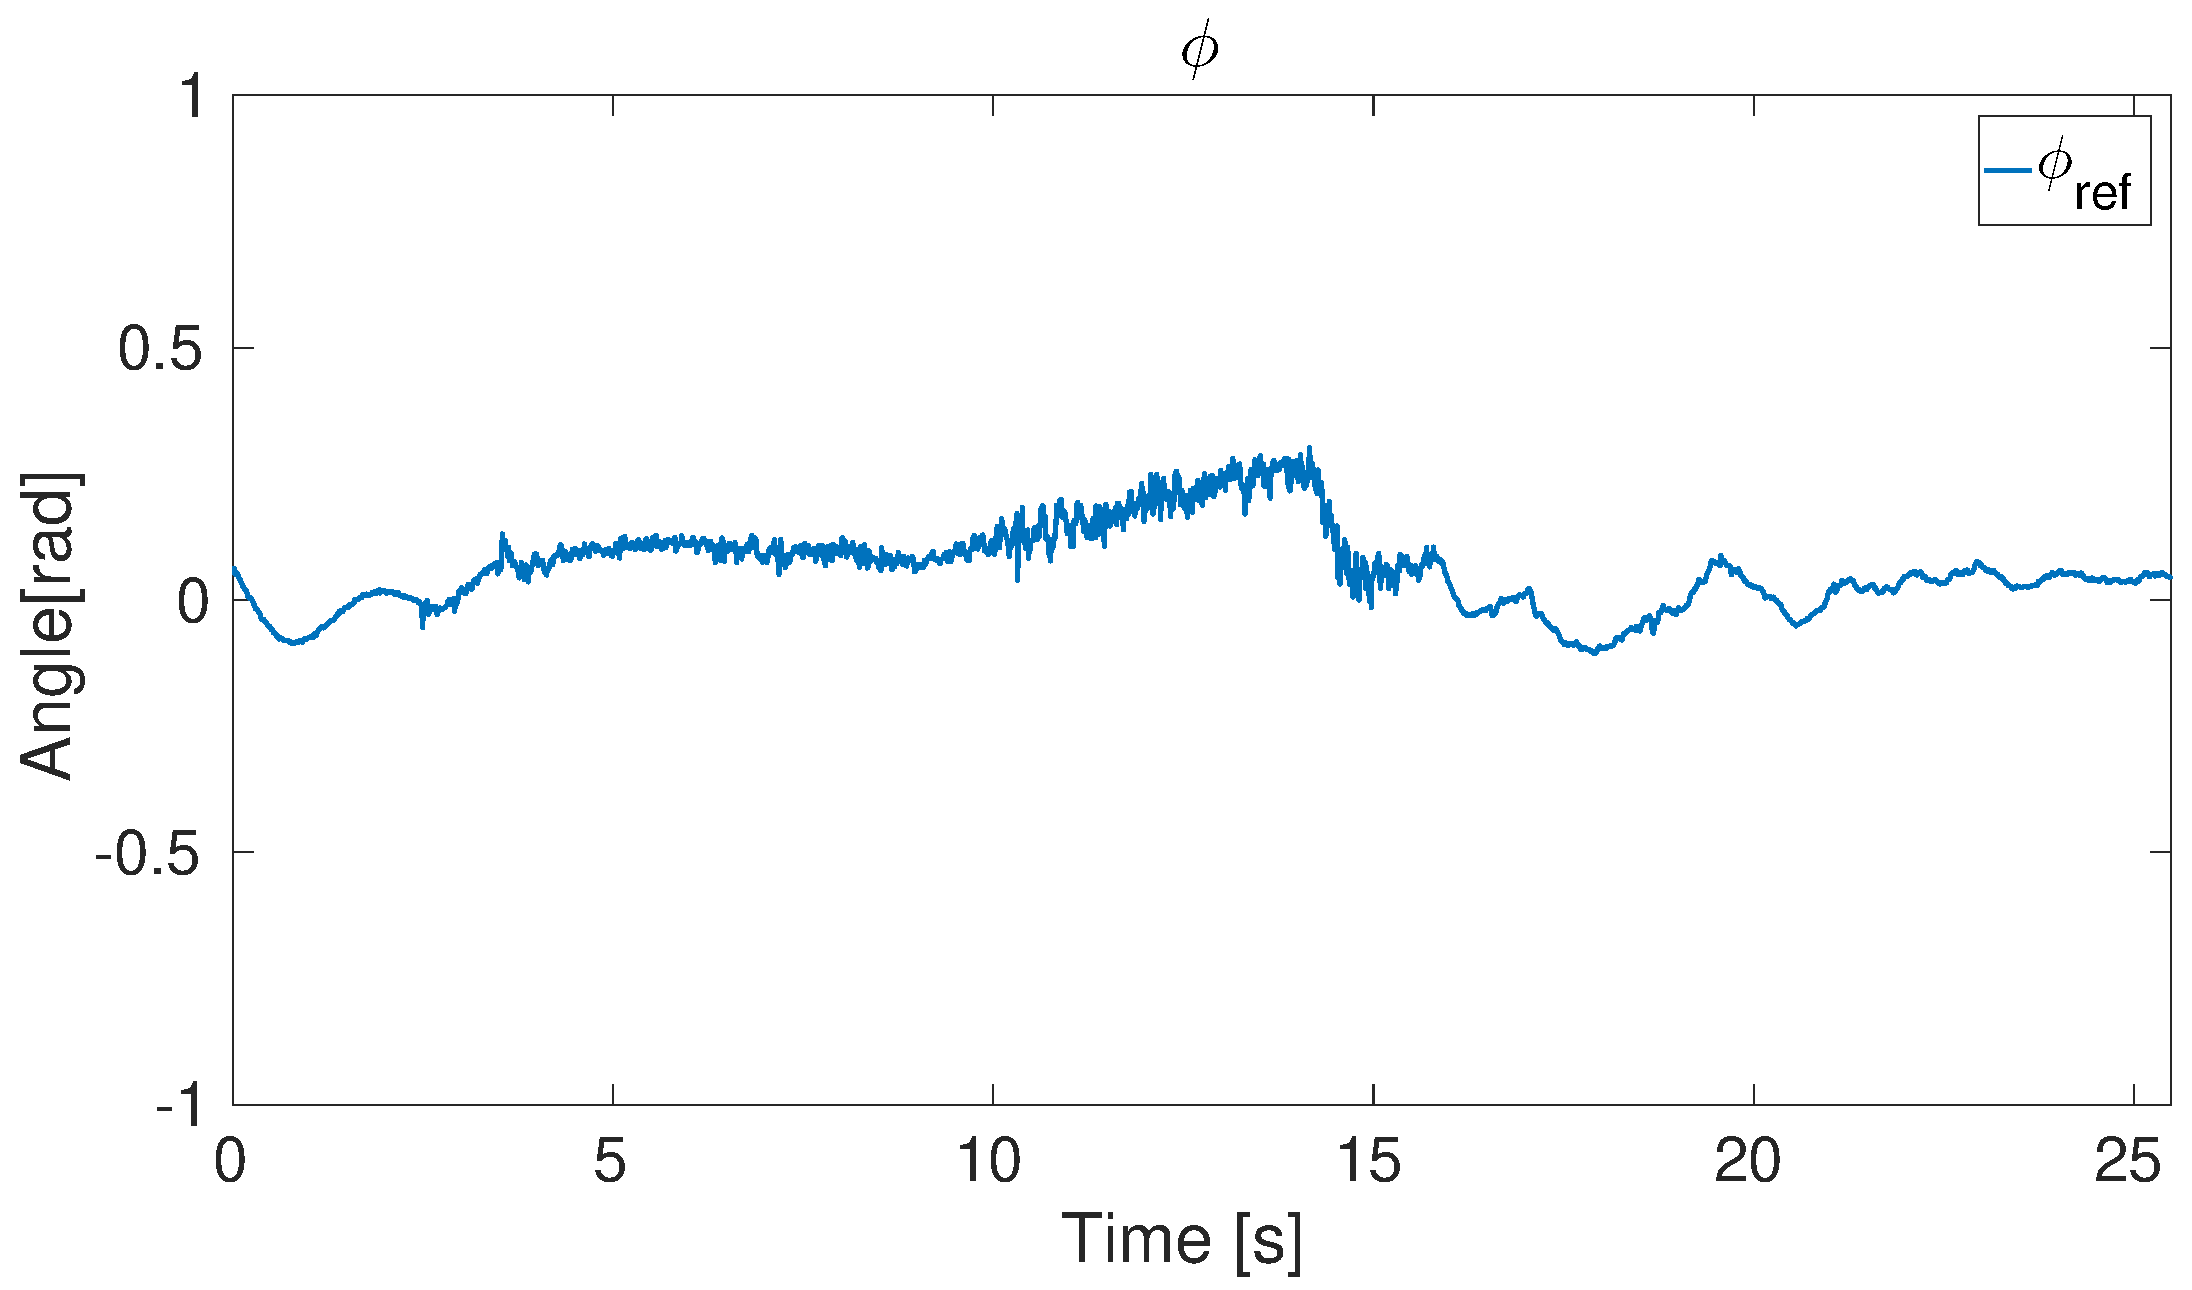
\includegraphics[width=0.7\textwidth]{testExactLinAttitudePhi}}
  \qquad
  \subfloat[][\label{fig:testExactAttitudePitch} The feedback linearisation in $\pitchAngle$.]{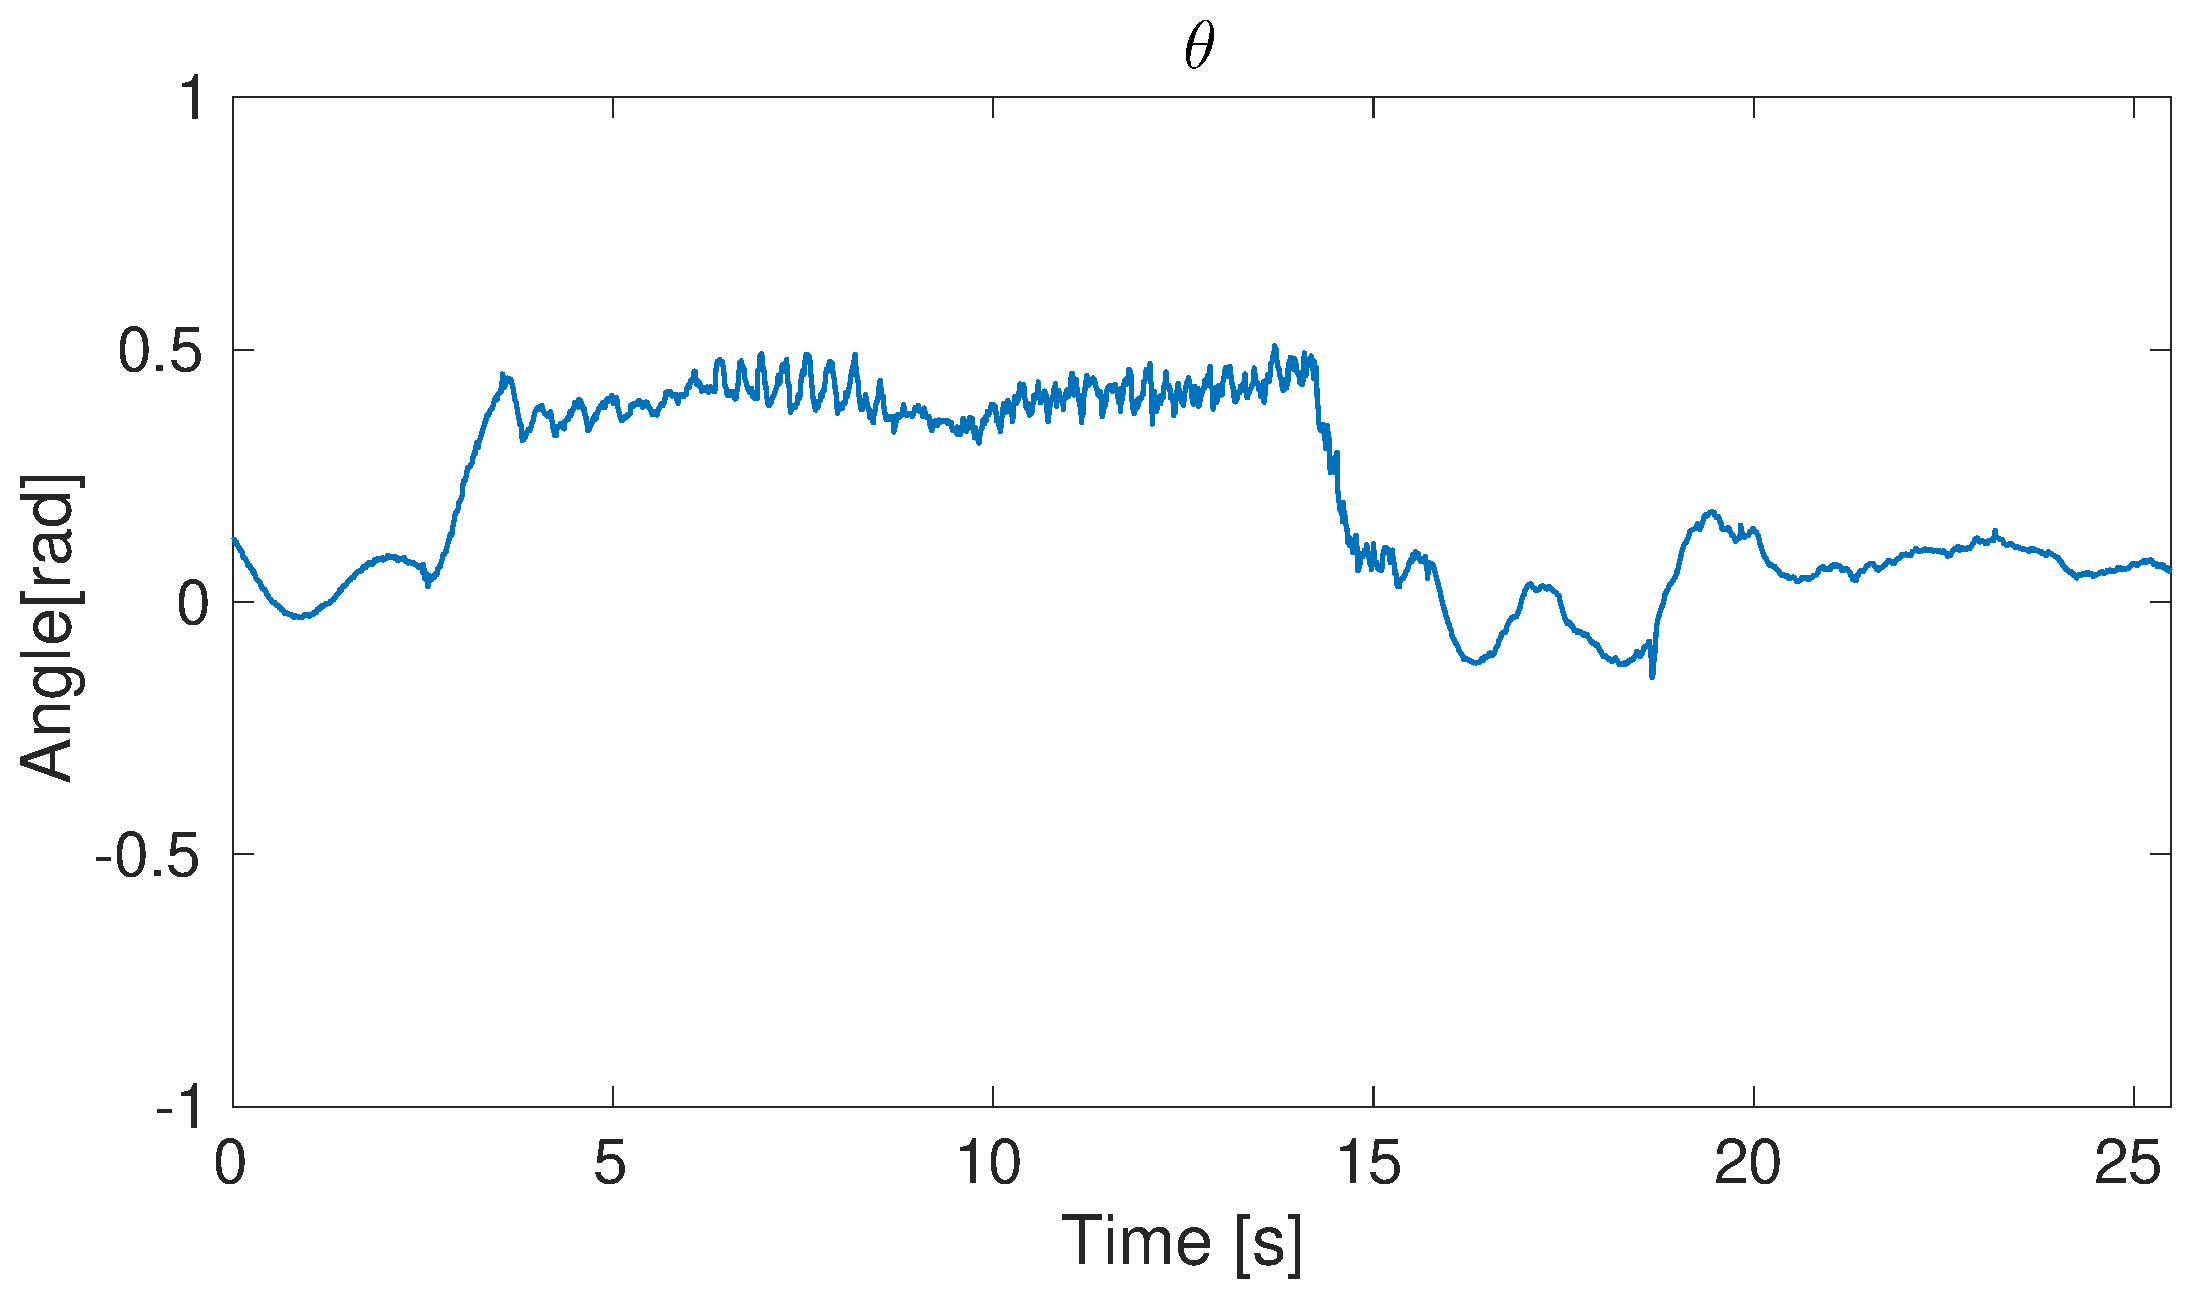
\includegraphics[width=0.7\textwidth]{testExactLinAttitudeTheta}}
  \qquad
  \subfloat[][\label{fig:testExactAttitudeYaw} The feedback linearisation in $\yawAngle$.]{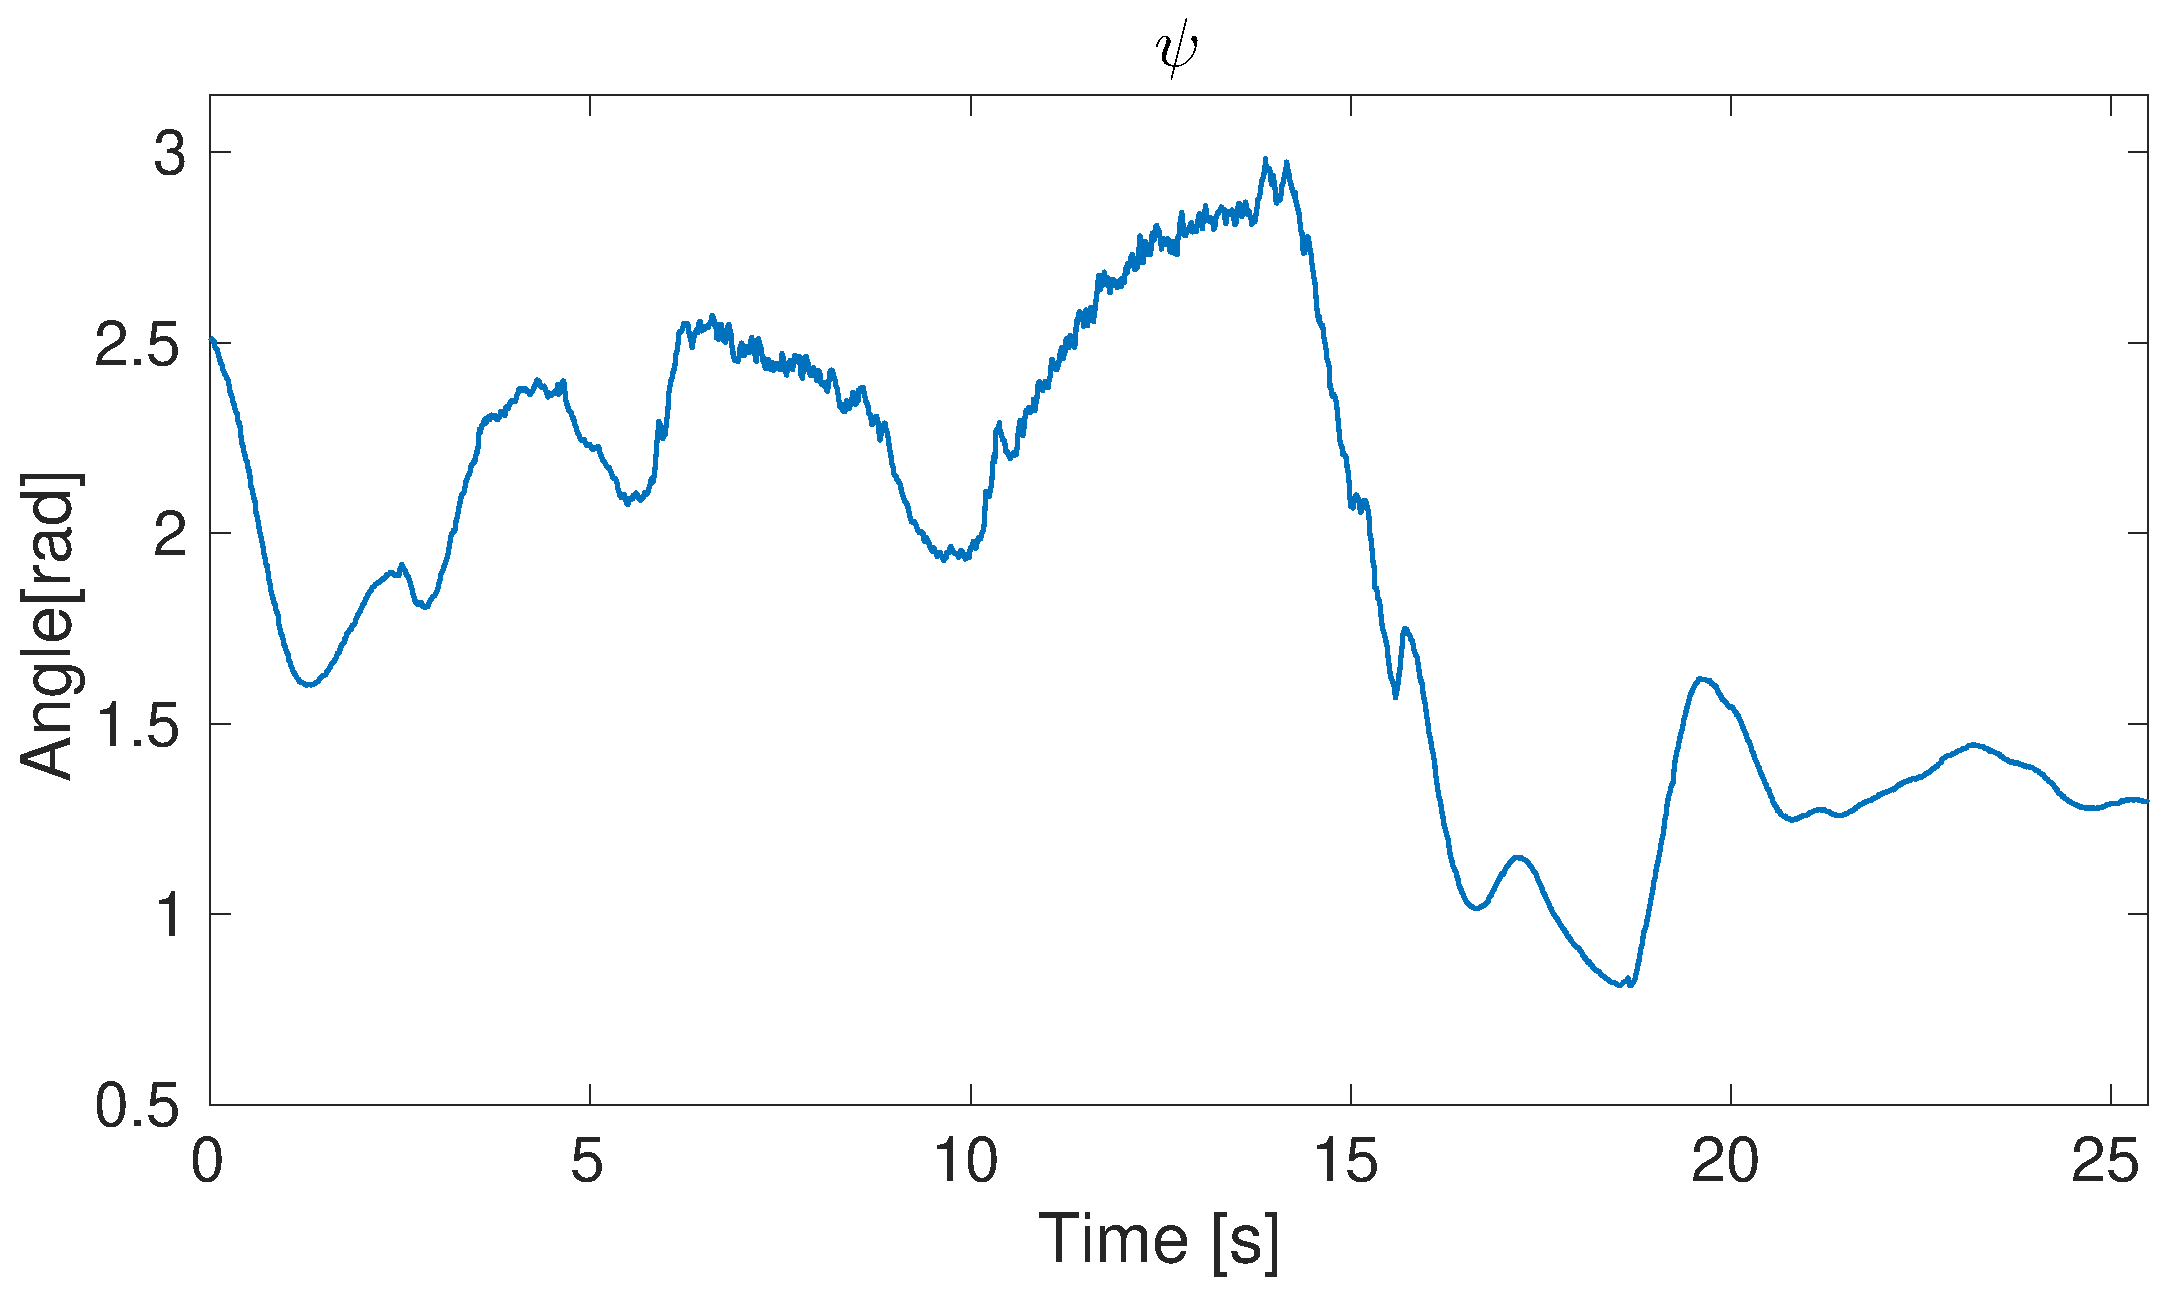
\includegraphics[width=0.7\textwidth]{testExactLinAttitudePsi}}
  \caption{\label{fig:ExactLinAttitude}% 
  The result of the feedback linearisation attitude controller with setpoints $\phi_{ref}=0$, $\theta_{ref}=0$ and $\psi_{ref}=0$. Note the instability in $\theta$ and $\psi$.}
\end{figure}

In general, comparisons of simulated tests and field tests gave mixed results.
In some test the field tests outperformed their simulated counterparts. This is probably due to the fact that damping parameters in the simulator were larger than the actual damping values of the system. The larger damping parameters in the simulation caused the simulated \abbrROV to be more heavily damped, which decreased the magnitude of overshoots and but increased the steady-state errors. The larger damping parameters may also explain the larger phase shift in the simulations of sine-signal tests.  

%A possible cause of the large parameter values might be the look-up table $\tau = f(u)$. If the look-up table returns a higher thrust than actually delivered, estimates of damping, inertia terms and the moment arm $z_b$ may be estimated with higher magnitudes. A possible way to bypass this is to model the thrusters using \begin{equation}
%\tau=C_{tau}u_{\text{Control}}\abs{u_{\text{Control}}}
%\end{equation} where $\tau$ is the thrust and $u_{\text{Control}}$ is the control signal sent to the thruster. 
%Another solution would be to upgrade the \abbrESC{}s to Blue\abbrESC{}s from Blue Robotics, since these can measure the rotations per minute (\abbrRPM) of the thruster \citep{bluerobotics}. This would enable the relation between \abbrRPM and thrust to be modelled and the \abbrRPM to be controlled for more predictable thruster performance.\todo[inline]{Hur ska detta tas upp? Blandar regulator- och estimeringsdiskussion.}

Overall, results were good in the view of the short amount of time available for controller tuning. The problem with the attitude controller and the linearising control law is unfortunate, but should be easily rectified with magnetometer calibration and some additional \abbrPID tweaking. Moreover, it is believed that exceptional angular velocity controller performance may be possible with further trimming.
